\documentclass[openany, a4paper, 10pt]{book}

\usepackage[style=numeric,sorting=none,block=space]{biblatex}
\addbibresource{report.bib}
\usepackage[english]{babel}

\usepackage{amsmath}
\usepackage{amsthm}
\usepackage{amsfonts}
\usepackage{amssymb}
\usepackage{array}
\usepackage{csquotes}
\usepackage{float}
\usepackage{microtype}
\usepackage{multirow}
\usepackage[symbol]{footmisc}
\usepackage[skins, breakable]{tcolorbox}
\usepackage{codestyle}
\usepackage[hscale=.7,vscale=.75]{geometry}
\usepackage[hidelinks]{hyperref}


\usetikzlibrary{graphs, graphs.standard, calc, shapes, arrows.meta}

\theoremstyle{plain}
\newtheorem{theorem}{Theorem}[chapter]

\theoremstyle{plain}
\newtheorem{proposition}[theorem]{Proposition}

\theoremstyle{plain}
\newtheorem{lemma}[theorem]{Lemma}

\theoremstyle{definition}
\newtheorem{definition}[theorem]{Definition}

\theoremstyle{plain}
\newtheorem{corollary}[theorem]{Corollary}

\theoremstyle{definition}
\newtheorem*{warning}{Warning}

\theoremstyle{remark}
\newtheorem*{remark}{Remark}

\renewcommand{\eqref}[1]{\hyperref[#1]{equation (\ref{#1})}}
\newcommand{\figref}[1]{\hyperref[#1]{Figure \ref{#1}}}
\newcommand{\tabref}[1]{\hyperref[#1]{Table \ref{#1}}}
\newcommand{\defref}[1]{\hyperref[#1]{Definition \ref{#1}}}
\newcommand{\theoref}[1]{\hyperref[#1]{Theorem \ref{#1}}}
\newcommand{\corref}[1]{\hyperref[#1]{Corollary \ref{#1}}}
\newcommand{\lemref}[1]{\hyperref[#1]{Lemma \ref{#1}}}
\newcommand{\secref}[1]{\hyperref[#1]{Section \ref{#1}}}
\newcommand{\chapref}[1]{\hyperref[#1]{Chapter \ref{#1}}}
\newcommand{\apref}[1]{\hyperref[#1]{Appendix \ref{#1}}}
\newcommand\compactcdots{\makebox[1em][c]{$\cdot$\hfil$\cdot$\hfil$\cdot$}}

\newenvironment{rcases}{\left.\begin{aligned}}{\end{aligned}\right\rbrace}

\interfootnotelinepenalty=10000

\newtcolorbox{examplebox}[1][]{
    enhanced,
    size=fbox,
    shadow={2.1mm}{-1.7mm}{0mm}{gray!20!white},
    before upper=\renewcommand\thempfootnote{\fnsymbol{mpfootnote}},
    boxrule={.5pt},
    colback=white,
    boxsep=10pt,
    left=5pt,
    right=5pt,
    sharp corners,
    breakable=true,
    #1
}

\newtcolorbox{cryptobox}[1][]{
    enhanced,
    size=fbox,
    before upper=\renewcommand\thempfootnote{\fnsymbol{mpfootnote}},
    boxrule={.5pt},
    colback=blue!8,
    boxsep=10pt,
    left=5pt,
    right=5pt,
    sharp corners,
    breakable=true,
    #1
}


\begin{document}


\begin{titlepage}
    \begin{center}
        {\makeatletter
            \fontsize{15}{15}\selectfont{L.J. Perrenet}
        \makeatother}

        \bigskip
        \bigskip
        \bigskip
        {\makeatletter
            \fontsize{20}{20}\selectfont{\textbf{Decoding CSIDH}}
        \makeatother}

        \vspace{.8em}
        {\makeatletter
            \fontsize{15}{15}\selectfont{\textbf{A Guide to Isogeny-Based Cryptography}}
        \makeatother}

        \bigskip
        \bigskip
        \bigskip
        \bigskip

        {\makeatletter
            \fontsize{15}{15}\selectfont{Master thesis,\\[.5em]Mathematisch Instituut, Universiteit Leiden.}
        \makeatother}

        \bigskip

        {\makeatletter
            \fontsize{15}{15}\selectfont{Supervised by Dr. S.A. Arpin.}
        \makeatother}

        \bigskip
        \bigskip

        {\makeatletter
            \fontsize{15}{15}\selectfont{July 22, 2024.}
        \makeatother}

        \vfill
        \begin{figure}[ht]
            \centering
            \includegraphics[width=.7\textwidth]{../build_plots/leiden_logo}
        \end{figure}
        \bigskip

        An uncompiled, \LaTeX\ version of this thesis is available at \url{https://github.com/jorisperrenet/MasterThesis}.
    \end{center}
\end{titlepage}

\chapter*{Abstract}
\addcontentsline{toc}{chapter}{Abstract}
In today's digital age, private communication is anchored in robust encryption techniques.
As the horizon of quantum computing draws nearer, current encryption methods may soon become vulnerable to quantum attacks, pointing to the need for post-quantum cryptography.
The CSIDH encryption scheme \cite{CSIDH}, grounded in isogeny-based cryptography, emerges as a compelling candidate for such post-quantum cryptography.
Understanding CSIDH requires a solid grasp of finite fields, number fields, and particularly elliptic curves.
This thesis strives to break down these topics to make the innovative CSIDH approach more accessible, encouraging further exploration in the field of isogeny-based cryptography to ensure digital privacy for years to come.


\chapter*{Introduction}
\addcontentsline{toc}{chapter}{Introduction}
In the world of digital communication, the robustness of encryption algorithms is of great concern.
Weak encryption algorithms pose a risk of sensitive information leakage, as messages could be decoded without our consent.
The digital era has made information rapidly accessible across great distances.
Yet, this convenience comes with a downside: the possibility of unauthorised interception by eavesdroppers.
Encrypting our messages is a very reliable measure to prevent such breaches.
However, the advent of quantum computing challenges our existing encryption methods, revealing susceptibilities to quantum attacks, highlighting the necessity for encryption methods that are resistant to such threats.
CSIDH \cite{CSIDH}, an encryption scheme founded on isogeny-based cryptography, is believed to be a promising example of such a quantum-resistant encryption scheme.
The method relies on mathematical theories and concepts such as finite fields, number fields, and elliptic curves.

Organised into five chapters (see \figref{hierarchy}), this thesis lays out the groundwork of algebraic structures relevant to CSIDH, aiming to provide an explanation of the CSIDH algorithm.
As a result, we hope to make the CSIDH algorithm more accessible in order to encourage further research in the area of isogeny-based cryptography, promoting the privacy of digital communication in the era of quantum computing.

\chapref{chap:finite_fields} introduces the concept of finite fields, as well as how to construct them.
The subsequent chapter is on number fields, number rings, and ideals, an important concept for understanding the CSIDH algorithm.
\chapref{chap:curves} focuses on elliptic curves, detailing their properties and establishing a basis for isogeny-based cryptography.
Elaborating on this theory, \chapref{chap:morphisms} explores isogenies, isomorphisms, and endomorphisms of elliptic curves.
This chapter further explores how ideals can act on elliptic curves, culminating in the introduction of isogeny graphs, an illustrative concept that helps with visualising isogeny-based cryptography.

The final chapter ties together the explored concepts, concentrating on their applications in encryption schemes.
It begins with an overview of the Diffie-Hellman key exchange, describing how two parties can reach a shared secret.
Subsequently, it presents the CSIDH encryption scheme, using the theory from the previous chapters.
Lastly, we discuss a variant of the CSIDH scheme, providing proofs and a way to break this variant if one can break CSIDH.

To further illustrate the inner workings of the CSIDH encryption scheme, we have implemented a generic, unoptimised version of the algorithm using SageMath \cite{sagemath}.
The computer code for this implementation is accessible in \apref{code} and on \url{https://github.com/jorisperrenet/MasterThesis}.

An alternative strategy for reading this thesis might be to begin with \secref{sec:CSIDH}, which explains the CSIDH encryption scheme.
By starting here, readers can grasp the ultimate objective and the requirements for achieving it.
They can then decide what sections and chapters to read to supplement their existing knowledge in order to understand the algorithm.

\begin{figure}[ht]
    \begin{center}
        \begin{tikzpicture}[block/.style={midway,align=center},scale=\textwidth/1.3cm]
            \draw (-.07,-.12) rectangle ++(1.07,.10) node[block] {\ref{chap:prelim}, \ref{chap:finite_fields}\\\hyperref[chap:prelim]{Preliminaries} \& \hyperref[chap:finite_fields]{Finite Fields}};
            \draw (-.07,0) rectangle ++(.56,.15) node[block] {\ref{sec:proj_space}, \ref{sec:curves}, \ref{sec:ec_over_ff}\\\hyperref[sec:proj_space]{Projective Plane}\\\hyperref[sec:curves]{Elliptic Curves} \hyperref[sec:ec_over_ff]{(over Finite Fields)}};
            \draw (.51,0) rectangle ++(.23,.32) node[block] {\ref{chap:number_fields}\\\hyperref[chap:number_fields]{Number Fields}\\\hyperref[chap:number_fields]{and Ideals}};
            \draw (.76,0) rectangle ++(.24,.49) node[block] {\ref{sec:diffie_hellman}\\\hyperref[sec:diffie_hellman]{Diffie-Hellman}\\\hyperref[sec:diffie_hellman]{Key Exchange}};
            \draw (-.07,.17) rectangle ++(.56,.15) node[block] {\ref{sec:isogenies}, \ref{sec:isom_classes}, \ref{sec:mont_curves}\\\hyperref[sec:isogenies]{Isogenies of Elliptic Curves}\\\hyperref[sec:isom_classes]{Isomorphism Classes of Elliptic Curves}};
            \draw (-.07,.34) rectangle ++(.81,.15) node[block] {\ref{sec:endomorphism_ring}, \ref{ideals_acting}\\\hyperref[sec:endomorphism_ring]{The Endomorphism Ring}\\\hyperref[ideals_acting]{Ideals Acting on Elliptic Curves}};
            \draw (-.07,.51) rectangle ++(1.07,.15) node[block] {\ref{sec:CSIDH}, \ref{gen_CSIDH}\\\hyperref[sec:CSIDH]{CSIDH}\\\hyperref[gen_CSIDH]{Variant of CSIDH}};
        \end{tikzpicture}
    \end{center}
    \vspace{-1em}
    \caption{The conceptual hierarchy of sections within this thesis is depicted as a series of rectangles, where a rectangle positioned above another indicates that the understanding of concepts introduced in the upper rectangle necessitates knowledge from the sections outlined in the lower rectangle.}
    \label{hierarchy}
\end{figure}

{
    \microtypesetup{protrusion=false}
    \hypersetup{linkcolor=black}
    \tableofcontents
}


\setcounter{chapter}{-1}
\chapter{Preliminaries}\label{chap:prelim}
This chapter aims to provide some of the background knowledge that the other chapters of this thesis rely on.
Before we move on to a couple of explicit definitions, we first state some topics that we regard as prerequisites to this thesis.
If the reader is not familiar with any of these subjects, they are referred to \cite{dictaat_dion}, \cite{dictaat_algebra_1}, or \cite{analysis} (depending on the subject).
We also note that online resources are readily available for most of these prerequisites.
In particular, we assume that the reader is familiar with (and has a thorough understanding of) the following.
\begin{itemize}
    \item The (set of all) integers $\mathbb Z$, the rationals $\mathbb Q$, and the reals $\mathbb R$.
    \item Prime numbers, divisors, prime factorisation, greatest common divisors, and the Euler totient function.
    \item Sets and subsets, as well as unions, intersections, differences, and the Cartesian product of sets together with the corresponding notation.
    \item The notation surrounding maps, the definition of one-to-one and bijective maps, the composition of maps, and the definitions of homomorphisms, isomorphisms, and endomorphisms.
    \item Addition and multiplication of polynomials, as well as knowing what coefficients and terms of a polynomial are.
    \item (Equivalence) relations, equivalence classes and the notation of basic propositional logic.
    \item Summations, linear combinations, (the dimension and rank of) vector spaces, and (the trace and determinant of) matrices.
    \item The basics of group actions, i.e., when is something a group action.
\end{itemize}


\section{Groups and Rings}
\begin{definition}
    A \textit{(binary) operation} on a set $G$ is a map $G \times G \to G$.
\end{definition}
\begin{definition}\label{is_a_group}
    A non-empty set $G$ with a binary operation on $G$, which we denote here as $\circ: G\times G \to G$, is called a \textit{group} if the following three requirements are met.
    \begin{itemize}
        \item (\textit{Associativity}) For all $a,b,c \in G$, one has $a \circ (b \circ c) = (a \circ b) \circ c$.
        \item (\textit{Identity element}) There is an $e \in G$ such that, for all $a \in G$, we have that $e \circ a = a \circ e = a$.
        \item (\textit{Inverse element}) For every $a \in G$ there exists an element $a^{-1} \in G$ such that $a \circ a^{-1} = a^{-1} \circ a = e$.
    \end{itemize}
    If $G$ is a group there is exactly one identity element in $G$, and every element of $G$ has exactly one inverse \cite[Theorem~2.4]{dictaat_dion}.
    Also, the group $G$ is called \textit{commutative} or \textit{abelian} if it satisfies the following additional requirement.
    \begin{itemize}
        \item (\textit{Commutativity}) For all $a,b \in G$ we have that $a \circ b = b \circ a$.
    \end{itemize}
    A non-empty subset $H$ of a group $G$ is called \textit{closed} under the operation $\circ$ if for any pair $(a, b) \in H \times H$ we have that $a \circ b \in H$ (where $\circ$ is the operation of the group $G$), and for any $a \in H$ we have that $a^{-1} \in H$ (where $a^{-1}$ is the inverse of $a$ in $G$).
    In that case, we call $H$ a \textit{subgroup} of $G$ as we can restrict $\circ$ to get a map $\circ: H \times H \to H$, yielding an operation on $H$.

    A \textit{finite group} is a group with only finitely many elements.
    The number of elements of a finite group is called its \textit{order}.
\end{definition}
\begin{definition}\label{fin_generated}
    A group $G$ under some operation is said to be \textit{finitely generated} if there is some finite subset of $G$ such that every element of $G$ can be written (under the group operation and taking inverses) as a combination of finitely many elements of the subset.
\end{definition}


\begin{definition}\label{is_a_ring}
    A non-empty set $R$ equipped with two binary operations, which we call \textit{addition} and \textit{multiplication} and denote by $+: R\times R \to R$ and $\cdot: R\times R \to R$ respectively, is called a \textit{ring} if the following requirements are met.
    \begin{itemize}
        \item The set $R$ is an abelian group under the $+$ operation (with the additive identity element denoted by $0$).
        \item The set $R$ is associative under multiplication and has a multiplicative identity element, which we denote by $1$ (also, we require that $0 \neq 1$ in this thesis).
        \item Multiplication in $R$ is distributive over addition, i.e., for every $a,b,c \in R$ we require that $a \cdot (b + c) = (a \cdot b) + (a \cdot c)$ and that $(b+c) \cdot a = (b\cdot a) + (c \cdot a)$.
    \end{itemize}
    A ring $R$ is called a \textit{commutative ring} if multiplication in $R$ is commutative.

    A subset $S$ of the ring $R$ is called a \textit{subring} of $R$ if $S$ contains the multiplicative identity of $R$ and $S$ is closed (\defref{is_a_group}) under the addition and multiplication operation (of the ring $R$).

    Just like with a group, a \textit{finite ring} is a ring with only finitely many elements. The number of elements of a finite ring is called its \textit{order}.
\end{definition}

\section{Modulo Arithmetic}
Let $n\mathbb Z = \{ nx: x \in \mathbb Z\}$ be a set under the usual addition and multiplication operations.

\begin{definition}
    Let $a,b \in \mathbb Z$ with $b > 0$ be arbitrary.
    Then, there exist unique \cite[Theorem~1.3]{dictaat_dion} integers $q$ and $r$ called the \textit{quotient} and \textit{remainder}, respectively, of the division of $a$ by $b$ such that $a=qb+r$ and $0 \leq r < b$.
\end{definition}

Fix $n$ to be a positive integer, in order to define the ring $\mathbb Z/n\mathbb Z$ we let $a$ and $b$ denote positive integers.
Define the relation $\sim$ between $a$ and $b$ such that $a \sim b \iff$ $a$ and $b$ have the same remainder after division by $n$.
This relation is an equivalence relation, and we call its equivalence classes \textit{residue classes modulo $n$}.
Since there are $n$ different remainders, there are exactly $n$ different residue classes modulo $n$.
We can now define $\mathbb Z/n\mathbb Z$ as the set containing the $n$ residue classes modulo $n$.
For any $a \in \mathbb Z$ we let $(a \bmod n)$ denote the residue class that contains $a$.
If $a$ and $b$ belong to the same residue class, i.e., $a \sim b$, we say that $a$ and $b$ are \textit{congruent} modulo $n$, and denote this by $a \equiv b \pmod n$.
We define the $+$ operator on $\mathbb Z/n \mathbb Z$ to be the map sending $((a \bmod n), (b \bmod n)) \to ((a+b) \bmod n)$, where the $+$ on the right-hand side is the ordinary addition taken in $\mathbb Z$.
Similarly, we let the $\cdot$ operator on $\mathbb Z/n \mathbb Z$ satisfy $(a \bmod n) \cdot (b \bmod n) = ((a\cdot b) \bmod n)$.
Under these two operations $\mathbb Z/n\mathbb Z$ forms a commutative ring.


\chapter{Finite Fields}\label{chap:finite_fields}
In many mathematical textbooks, the theory of finite fields is considered to be a prerequisite.
This causes most books to be unsuitable for learning from top to bottom to the ones that do not grasp the full scope of finite fields.
With that in mind, this chapter aims to provide a thorough explanation of the theory on finite fields, as we will use it in later parts of this thesis.

Commencing with fundamental principles that define a finite field, this chapter progressively reveals the existence and creation of finite fields.
Although this chapter introduces the subject quite extensively, it is still focused on providing background for the rest of the thesis.
Therefore, not all the existing theory on finite fields is stated.
If the reader is interested in a more complete theory, they are encouraged to consult \cite{huo_ff}, \cite{niederreiter}, and \cite{kochendorffer}.


\section{Fields}
\begin{definition}\label{is_a_field}
    A non-empty set $F$ equipped with two binary operations, which we call \textit{addition} and \textit{multiplication} and denote by $+: F\times F \to F$ and $\cdot: F\times F \to F$ respectively, is called a \textit{field} if the following requirements are met.
    \begin{itemize}
        \item The set $F$ is an abelian group under the $+$ operation (with the additive identity element denoted by $0$).
        \item The set $F\setminus \{ 0 \}$ is an abelian group under the $\cdot$ operation (we usually denote this group as $F^*$ and denote its multiplicative identity element as $1$).
        \item Multiplication in $F$ is distributive over addition, i.e., for every $a,b,c \in F$ we require that $a \cdot (b + c) = (a \cdot b) + (a \cdot c)$ and that $(b+c) \cdot a = (b\cdot a) + (c \cdot a)$.
    \end{itemize}
    A subset $K$ of the field $F$ is called a \textit{subfield} of $F$ if $K$ is a field with respect to the addition and multiplication operation (of the field $F$).
    If $K$ is a subfield of $F$, then $F$ is called an \textit{extension (field)} of $K$.
\end{definition}
\begin{remark}
    Equivalently, a field $F$ is a commutative ring (\defref{is_a_ring}) where $0 \neq 1$ and all elements of $F \setminus \{ 0 \}$ are invertible (i.e., have an inverse element in $F \setminus \{ 0 \}$) under multiplication.
\end{remark}
\begin{remark}
    Similar to groups and rings, a field is called a \textit{finite field} if it has finitely many elements.
    The number of elements of a finite field $F$ is called its \textit{order}.
\end{remark}

\begin{examplebox}[label={first_example}, nameref={our previous example}]
    With respect to our usual addition and multiplication operation, it can be shown that $\mathbb Q$, $\mathbb R$, and $\mathbb Z / 7 \mathbb Z$ are fields.

    Additionally, we can see that $\mathbb Z$ is not a field as $\mathbb Z\setminus \{0\}$ does not contain an inverse element for any numbers except $-1$ and $1$.
    To motivate this, note that $\mathbb Z \subset \mathbb Q$.
    Now, if $\mathbb Z$ is a field then it will be a subfield of $\mathbb Q$ as $\mathbb Q$ is a field with the same operations.
    As $\mathbb Q \setminus \{ 0 \}$ is a group with respect to multiplication (since $\mathbb Q$ is a field) we find that $2 \in \mathbb Q$ has a unique inverse.
    Since $1$ is the multiplicative identity of $\mathbb Q$ we know that the unique inverse of $2$ must equal $1/2 \in \mathbb Q$.
    Now, $1/2 \notin \mathbb Z$, contradicting the fact that $\mathbb Z$ contains an inverse element for $2 \in \mathbb Z$.
    Therefore, $\mathbb Z$ cannot be a subfield of $\mathbb Q$, and in turn $\mathbb Z$ cannot be a field.

    Likewise, $(\mathbb Z / 12 \mathbb Z)^*$ does not contain an inverse element for the residue class $(3 \bmod 12)$ as we can not find an $x\in \mathbb Z$ such that $3x \equiv 1 \pmod {12}$.
    We can conclude that $\mathbb Z / 12 \mathbb Z$ is not a (finite) field.


\end{examplebox}

\begin{theorem}\label{prime_field}
    Let $n$ be a positive integer. Then $\mathbb Z / n \mathbb Z$ is a finite field if and only if $n$ is prime.
\end{theorem}
\begin{proof}
    First, let $n$ be a positive integer, but not a prime.
    To prove necessity, we assume that $\mathbb Z/n\mathbb Z$ is a finite field and prove that it leads to a contradiction.
    Since $n$ is not prime, there exists an integer $d$ such that $1 < \gcd(d, n) < n$.
    For any such $d$, let $a \in (\mathbb Z/n\mathbb Z)^*$ denote the multiplicative inverse of ($d \bmod n$), note that this inverse exists by our assumption that $\mathbb Z/n\mathbb Z$ is a finite field.
    Since $a$ is the inverse of ($d \bmod n$) we know that $(d \bmod n) \cdot a = (1 \bmod n)$.
    Let $a' \in \mathbb Z$ be an element of the residue class of $a$, we find that there exists some integer $b$ such that $d\cdot a' - b\cdot n = 1$.
    We know that $\gcd(d, n)$ divides both $d$ and $n$, thus it divides the left-hand side of our equation, implying that it must also divide $1$.
    Since $\gcd(d, n) > 1$ we know that the equation cannot hold, resulting in a contradiction.
    Therefore, $\mathbb Z/n\mathbb Z$ can only be a finite field if $n$ is prime.
    A proof of sufficiency can be found in \cite[Theorem~3]{MIT_finite_fields} and in \cite[Theorem~7.5]{Forney_finite_fields}.
\end{proof}
\begin{examplebox}
    In \nameref{first_example} we have stated that $\mathbb Z/7\mathbb Z$ is a field.
    In fact, this is a direct consequence of \theoref{prime_field}.
    In this example, we will show that $\mathbb Z / 7 \mathbb Z$ is a field using brute force calculations.

    First, let 0 through 6 denote the elements of $\mathbb Z / 7 \mathbb Z$ (where each number is used to denote the residue class that contains it).
    We will get the following addition and multiplication tables concerning these elements:
    \begin{figure}[H]
        \centering
        \begin{minipage}{.5\textwidth}
            \centering
            \begin{tabular}{c|ccccccc}
                $+$ & 0 & 1 & 2 & 3 & 4 & 5 & 6 \\
                \hline
                0 & 0 & 1 & 2 & 3 & 4 & 5 & 6 \\
                1 & 1 & 2 & 3 & 4 & 5 & 6 & 0 \\
                2 & 2 & 3 & 4 & 5 & 6 & 0 & 1 \\
                3 & 3 & 4 & 5 & 6 & 0 & 1 & 2 \\
                4 & 4 & 5 & 6 & 0 & 1 & 2 & 3 \\
                5 & 5 & 6 & 0 & 1 & 2 & 3 & 4 \\
                6 & 6 & 0 & 1 & 2 & 3 & 4 & 5 \\
            \end{tabular}
        \end{minipage}%
        \begin{minipage}{.5\textwidth}
            \centering
            \begin{tabular}{c|ccccccc}
                $\cdot$ & 0 & 1 & 2 & 3 & 4 & 5 & 6 \\
                \hline
                0 & 0 & 0 & 0 & 0 & 0 & 0 & 0 \\
                1 & 0 & 1 & 2 & 3 & 4 & 5 & 6 \\
                2 & 0 & 2 & 4 & 6 & 1 & 3 & 5 \\
                3 & 0 & 3 & 6 & 2 & 5 & 1 & 4 \\
                4 & 0 & 4 & 1 & 5 & 2 & 6 & 3 \\
                5 & 0 & 5 & 3 & 1 & 6 & 4 & 2 \\
                6 & 0 & 6 & 5 & 4 & 3 & 2 & 1 \\
            \end{tabular}
        \end{minipage}
        \vspace{-.5em}
    \end{figure}
    For the abelian group (\defref{is_a_group}) with respect to addition, we verify the following.
    \begin{itemize}
        \item[--] Identity element: It is clear that $0$ is our identity element, and that $0 + a = a + 0 = a$ holds for all $a\in \mathbb Z / 7 \mathbb Z$.
        \item[--] Inverse element: The addition table has one, and exactly one, $0$ on each of its rows and columns.
            Upon looking in the row of some $a\in \mathbb Z / 7 \mathbb Z$,
            there will be an element $b\in (\mathbb Z / 7 \mathbb Z)$ such that $a+b=0$ (the element $b$ can be found in the column containing the 0).
        \item[--] Commutativity: The addition table is symmetric around its main diagonal, we must thus have that for all $a,b\in \mathbb Z / 7 \mathbb Z$, the equality $a+b = b+a$ holds.
        \item[--] Associativity: Let $a,b,c \in \mathbb Z / 7 \mathbb Z$, then $(a+b)+c = a+(b+c)$ holds.
            This can be seen by verifying all possible $a$, $b$, and $c$.
    \end{itemize}
    For the abelian group $(\mathbb Z / 7 \mathbb Z) \setminus \{ 0 \}$ with respect to multiplication:
    \begin{itemize}
        \item[--] Identity element: It is clear that $1$ is our identity element, and that $1 \cdot a = a \cdot 1 = a$ holds for all $a\in \mathbb Z / 7 \mathbb Z$.
        \item[--] Inverse element: The inverse of an element can be found by first finding the $1$ in its row and subsequently looking at the column that contains the $1$.
        \item[--] Commutativity: The multiplication table is likewise symmetric around its main diagonal, commutativity follows.
        \item[--] Associativity: Let $a,b,c \in (\mathbb Z / 7 \mathbb Z) \setminus \{ 0 \}$, then $(a\cdot b)\cdot c = a\cdot (b\cdot c)$ holds.
            This can be seen by verifying all possible $a$, $b$, and $c$.
    \end{itemize}
    Finally, the distributive property of $\mathbb Z / 7 \mathbb Z$ can be verified by checking all possibilities.
    We now know that $\mathbb Z / 7 \mathbb Z$ is a (finite) field due to \defref{is_a_field}.
\end{examplebox}


As we shall see in \theoref{theo:ff}, it turns out that there only exist finite fields with $p^m$ elements, for any prime $p$ and positive integer $m$.
The finite field of that order is denoted as $\mathbb F_{p^m}$.
Moreover, any two fields of order $p^m$ are isomorphic.
We already know that for $m=1$ the set
$\mathbb F_p:= \mathbb Z/p\mathbb Z$ is a finite field due to \theoref{prime_field},
however constructing finite fields for integers $m > 1$ requires a little more effort.


\section{Polynomial Rings}\label{sec:pol_rings}
For this entire section, we let $p$ denote a prime number and $R$ a commutative ring (\defref{is_a_ring}).
Note that any field is also a commutative ring.

\begin{definition}\label{pol_ring}
    We define the \textit{polynomial ring} $R[x]$ for any commutative ring $R$ as the set of all polynomials in $x$ (with finitely many terms) with coefficients in $R$ (note that $x$ is a variable and its value does not need to be in $R$).
    Let $n$ be a non-negative integer, using our definition of $R[x]$ we say that the set
    \begin{equation}\label{pol_sets}
        \left\{ \sum_{i=0}^n a_i x^i, \quad \text{with } a_0, a_1, \dots, a_{n-1} \in R \text{ and } a_n \in R\setminus \{ 0 \} \right\}
    \end{equation}
    contains all polynomials $f \in R[x]$ of \textit{degree} $n$.
    Generally, the degree of a polynomial $f \in R[x]$ is denoted as $\deg(f)$.
    Furthermore, we define the degree of the \textit{zero polynomial}, i.e., the polynomial $0 \in R[x]$, to be $-\infty$\footnote[1]{
        This definition is not used throughout all literature,
        sometimes the degree of the zero polynomial is defined to be non-existent.
    }.
    Building on \eqref{pol_sets}, we call $a_n$ the \textit{lead coefficient} of a polynomial in any such set.
    A polynomial is called \textit{monic} if its lead coefficient equals $1$.

    Equivalently, we can define $R[x]$ as the union of all sets from \eqref{pol_sets} for arbitrary non-negative integers $n$ together with the zero polynomial.
\end{definition}
\begin{remark}
    If $f$ is a polynomial in a polynomial ring $R[x]$, then we use the notation
    $f$ and $f(x)$ interchangeably in this thesis to denote the polynomial.
\end{remark}

Multiplication and addition (denoted by $\cdot$ and $+$, respectively) in this polynomial ring work as expected.
\begin{examplebox}
    Define two polynomials $f(x)=3x^8+6 \in \mathbb F_7[x]$ and $g(x) = x^2 + 2x + 1 \in \mathbb F_7[x]$.
    Using \defref{pol_ring} we find that $\deg(f) = 8$, $\deg(g)=2$, $f$ has lead coefficient 3, and $g$ is monic.
    Also, $f(x) + g(x) = 3x^8 + x^2 + 2x \in \mathbb F_7[x]$ and
    $f(x) \cdot g(x) = 3x^{10} + 6x^9 + 3x^8 + 6x^2 + 5x + 6 \in \mathbb F_7[x]$.
\end{examplebox}

\begin{definition}\label{quot_rem}
    Let $f \in R[x]$ be an arbitrary polynomial.
    For all polynomials $g \in R[x]\setminus \{ 0 \}$ (i.e., excluding the zero polynomial)
    there exist unique \cite[Theorem~3.16]{unique_quotient} polynomials $q,r \in R[x]$ such that $\deg(r) < \deg(g)$ and $f(x) = q(x)g(x) + r(x)$.
    These polynomials are called the \textit{quotient} and \textit{remainder}, respectively, of the division of $f(x)$ by $g(x)$ (this division is sometimes denoted as $f(x)/g(x)$).
\end{definition}

\begin{examplebox}[label={long_div_ex}, nameref={long division example}]
    In this example, we determine the quotient and the remainder of
    $f(x)/g(x)$ using long division where
    $f(x)=9x^5 + 3x^4 + 5x^3 + 6x^2 + 8x + 1$ and
    $g(x)=2x^3 + x^2 + 7$ are both elements of $\mathbb F_{11}[x]$.
    For the first step, we note that $10\cdot (2x^3 + x^2 + 7) = 9x^3 + 10x^2 + 4$.
    Remember that all coefficients of these polynomials are in $\mathbb F_{11}$.\footnote[2]{
        This is the Dutch notational variant of long division or ``staartdeling''.
        The denominator is written down left of the $/$,
        the numerator comes next
        and after the $\backslash$ the quotient is denoted
        element by element.
        The denominator is multiplied by the first element
        of the quotient (which one needs to figure out and write down), this is then subtracted from the numerator
        and the result is written below a long horizontal line.
        Now the result becomes the new numerator and the process is repeated.
        At the end you can find the remainder of the division at the bottom and the quotient at the top right.
    }
    \begin{alignat*}{8}
        2x^3 + x^2 + 7 /&  9x^5  &+&&  3&x^4  &+&  5x^3  &+&  6x^2  &+&  8x  &+&  1  & \backslash 10x^2 + 2x + 7 \\[-.3em]
                        &  9x^5  &+&& 10&x^4  & &        &+&  4x^2  & &      & &     &\\[-1em] \cline{2-14} \\[-2em]
                        &        & &&  4&x^4  &+&  5x^3  &+&  2x^2  &+&  8x  &+&  1  &\\[-.3em]
                        &        & &&  4&x^4  &+&  2x^3  & &        &+&  3x  & &     &\\[-1em] \cline{5-14} \\[-2em]
                        &        & &&   &     & &  3x^3  &+&  2x^2  &+&  5x  &+&  1  &\\[-.3em]
                        &        & &&   &     & &  3x^3  &+&  7x^2  & &      &+&  5  &\\[-1em] \cline{8-14} \\[-2em]
                        &        & &&   &     & &        & &  6x^2  &+&  5x  &+&  7  &
    \end{alignat*}
    Therefore, we can write $f(x) = q(x)g(x) + r(x)$ with $q(x) = 10x^2+2x+7$ and $r(x)=6x^2+5x+7$.
    Note that $\deg(r) < \deg(g)$ indeed holds.
    If $\deg(r) \geq \deg(g)$, we should have continued the long division by removing additional factors of $g(x)$ from the leftover $r(x)$ until $\deg(r) < \deg(g)$ is satisfied.
\end{examplebox}

\begin{definition}\label{is_irreducible}
    A non-constant (i.e., of degree at least 1) polynomial $f \in R[x]$ is called \textit{irreducible} if there
    does not exist a polynomial $g \in R[x]$ such that $0 < \deg(g) < \deg(f)$
    and the remainder of $f(x)/g(x)$ is the zero polynomial.
\end{definition}
Now that we have provided some definitions regarding polynomial rings $R[x]$ for any commutative ring $R$ (which will be needed in upcoming chapters), we start by stating theorems concerning only $\mathbb F_p[x]$ (this does not mean that some theorems do not generalise to other polynomial rings).

Similar to how non-zero integers can be uniquely factored into products of prime numbers and $-1$,
non-zero polynomials $f \in \mathbb F_p[x]$ can be uniquely factored into products of monic irreducible polynomials and a constant in $\mathbb F_p^*$ \cite[Theorem~1.2.17]{dictaat_joost}.

\begin{examplebox}
    The polynomial $f(x)=2x^2+x+1$ in $\mathbb F_3[x]$ is irreducible.
    To illustrate this, we write it in the form $q(x) g(x) + r(x)$ where $g(x)$ iterates through all possible polynomials in $\mathbb F_3[x]$ with $0 < \deg(g) < \deg(f)$:
    \vspace{-.5em}
    {\allowdisplaybreaks\begin{alignat*}{3}
        (2x+1    )(x   ) + 1 &&       && (x+2     )(2x  ) + 1& \\
        (2x+2    )(x +1) + 2 &&       && (x       )(2x+1) + 1& \\
        (2x      )(x +2) + 1 &&\qquad && (x+1     )(2x+2) + 2&.
    \end{alignat*}
    }%
    \vspace{-.5em}
    No remainder equals the zero polynomial, $f(x)$ is thus irreducible.\footnote{
        A faster way to check irreducibility of a polynomial $f(x) \in \mathbb F_p[x]$ with $\deg(f) \geq 2$
        is to check for roots.
        That is, if $f(x)$ is irreducible then there does not exist an $a \in \mathbb F_p$
        such that $f(a) = 0$.
        The converse only holds if $f(x)$ is a polynomial of degree 2 or 3.
    }
    \tcbline
    The polynomial $f(x)=x^3+x+1$ is not irreducible in $\mathbb F_3[x]$.
    It can be expressed as the product of two polynomials $p(x)=x+2$ and $q(x)=x^2+x+2$ of non-zero degree.
    The remainder of dividing $f(x)$ by either $p(x)$ or $q(x)$ will result in the zero polynomial.
    \tcbline
    In $\mathbb F_{19}[x]$, the polynomial
    $f(x) = 4x^{11} + 5x^3 + 13x^2 + 7x + 15$
    is not irreducible.
    The unique factorisation (up to permutation of the factors) of $f(x)$ equals
    \begin{equation*}
        (4)(x + 9)(x^2 + 10x + 3)(x^3 + 15x^2 + 17)(x^5 + 4x^4 + 18x^3 + 9x^2 + 10x + 6)
    \end{equation*}
    and is thus the product of monic irreducible polynomials in $\mathbb F_{19}[x]$ multiplied by the constant $4\in \mathbb F_{19}^*$.
    Or, as you can also see it, the polynomial $4 \in \mathbb F_{19}[x]$ of degree 0.
\end{examplebox}


\begin{definition}\label{pol_mods}
    Let $f,g \in \mathbb F_p[x]$ be arbitrary and fix $h \in \mathbb F_p[x] \setminus \{ 0 \}$.
    We say that $f$ and $g$ are \textit{congruent} modulo $h$ if the remainder of $f(x)/h(x)$ equals the remainder of $g(x)/h(x)$.
    This congruence is denoted as $g \equiv f \pmod h$ and forms an equivalence relation.
    We denote the equivalence classes of this relation by $(f \bmod h)$.
    The set of all these equivalence classes is denoted by $\mathbb F_p[x]/(h)$.
\end{definition}
Following the notation of the definition, one can define the $+$ operation on $\mathbb F_p[x]/(h)$ by the map $((f \bmod h), (g \bmod h)) \to ((f+g) \bmod h)$, where $f+g$ is evaluated using polynomial addition.
Similarly, one can let the $\cdot$ operation satisfy $(f \bmod h) \cdot (g \bmod h) = ((f \cdot g) \bmod h)$.
Equipped with the $+$ and $\cdot$ operator, $\mathbb F_p[x]/(h)$ forms a commutative ring \cite[Theorem~1.3.8]{dictaat_joost}.


\begin{examplebox}
    Let
    $f(x)=9x^5 + 3x^4 + 5x^3 + 6x^2 + 8x + 1$ and
    $g(x)=2x^3 + x^2 + 7$ be defined over $\mathbb F_{11}[x]$
    (note that these are the same polynomials as in the \nameref{long_div_ex}).
    We can write $f(x) = q(x)g(x) + r(x)$ with $q(x) = 10x^2+2x+7$ and $r(x)=6x^2+5x+7$.

    Furthermore,
    \begin{equation*}
        r(x) + g(x) \equiv 2x^3+7x^2+5x+3 \equiv 6x^2 + 5x + 7 \equiv r(x) \pmod {g(x)}.
    \end{equation*}
    Likewise, each intermediate result in the previous \nameref{long_div_ex} is contained in $(r \bmod g)$
    as in the process of the long division we only subtracted multiples of $g$ from the original polynomial $f$.
\end{examplebox}

\section{Finite Fields of \texorpdfstring{$p^m$}{pm} Elements}
Combining our theory on fields and polynomial rings, we are able to construct finite fields of $p^m$ elements, where $p$ is a prime number and $m$ is a positive integer.
\begin{theorem}\label{ff_from_polrings}
    Fix $p$ to be a prime number and let $g \in \mathbb F_p[x]$ be an irreducible polynomial of degree $m$.
    Following the notation from \defref{pol_mods}, we find that $\mathbb F_p[x]/(g)$ forms a finite field of order $p^m$.
\end{theorem}
\begin{proof}
    A proof can be found in \cite[Theorem~7.9]{Forney_finite_fields} or in
    \cite[Theorems~1.3.13,1.3.15]{dictaat_joost}.
\end{proof}
\begin{theorem}
    There exists at least one irreducible polynomial
    $g \in \mathbb F_p[x]$ of degree $m$
    for every integer $m \geq 1$ and every prime $p$.
\end{theorem}
\begin{proof}
    For a proof, the reader is referred to \cite[Theorem~2.6.6]{dictaat_joost} or \cite[Lemma~1.4]{huo_ff}.
\end{proof}
\begin{theorem}\label{theo:ff}
    Every finite field $F$ is isomorphic to a finite field $\mathbb F_p[x]/(g)$ constructed by an irreducible polynomial $g \in \mathbb F_p[x]$.
    Moreover, for every prime $p$ and every integer $m \geq 1$ there exists exactly one finite field with $p^m$ elements up to isomorphism, meaning that one can always find an isomorphism between two finite fields of $p^m$ elements. Finite fields with an order that can not be written as the power of a prime, i.e., in the form $p^m$, do not exist.
\end{theorem}
\begin{proof}
    Proofs of this theorem can be found in
    \cite[Section~1.1~up~to~Theorem~1.2]{huo_ff}, \cite[Theorems~7.16,7.18]{Forney_finite_fields}, and
    \cite[Theorems~2.6.2,2.8.9]{dictaat_joost}.
\end{proof}

\begin{theorem}
    Under multiplication $\mathbb F_{p^m}^*$ forms a cyclic group,
    i.e., there exists an element $\alpha \in \mathbb F_{p^m}^*$ such that $\mathbb F_{p^m}^* = \{1, \alpha, \dots, \alpha^{p^m-2} \}$.
    Such an element is called a \textit{primitive element}\footnote[2]{
        It is said that a primitive element of $\mathbb F_{p^m}$ is a \textit{generator} of $\mathbb F_{p^m}^*$.
        Conversely, each generator of $\mathbb F_{p^m}^*$ is called a \textit{primitive element} of $\mathbb F_{p^m}$.
    }, and
    there are exactly $\varphi(p^m-1)>0$ distinct primitive elements in $\mathbb F_{p^m}^*$ where $\varphi$ denotes Euler's totient function.
\end{theorem}
\begin{proof}
    A proof that $\mathbb F_{p^m}^*$ is cyclic and generated by primitive elements is contained in \cite[Theorem~1.3]{huo_ff}.
    For the number of distinct primitive elements, the reader is referred to \cite[Theorem~7.13]{Forney_finite_fields}.
\end{proof}

Also, under addition $\mathbb F_{p^m}$ is isomorphic to the vector space $(\mathbb F_p)^m$, meaning that we can represent every polynomial $g \in \mathbb F_p[x]/(f)$ (where $f$ is an irreducible polynomial in $\mathbb F_p[x]$ of degree $m$) as a vector.
For example, $g(x)=(x^3+2x+1 \bmod f)\in \mathbb F_3[x]/(f)$ with $f = x^4+x+2$ can be represented as \texttt{1021}, where each term (from highest to lowest degree) has an entry equal to their coefficient in $g(x)$.

\begin{examplebox}
    We would like to illustrate some properties of $\mathbb F_8$ by highlighting them in the following example.
    \nocite{finite_fields_example}

    We take the irreducible polynomial $f(x):=x^3+x^2+1 \in \mathbb F_2[x]$ and write down the elements of $\mathbb F_2[x]/(f)$ (note that by \theoref{ff_from_polrings} this is a finite field of order 8), to get
    \begin{gather*}
        (0\bmod f), (1 \bmod f), (x\bmod f), (x+1\bmod f), (x^2\bmod f), \\
        (x^2+1\bmod f), (x^2+x\bmod f),\text{ and }(x^2+x+1\bmod f).
    \end{gather*}
    In vector notation, these can be denoted by $\texttt{000}, \texttt{001}, \texttt{010}, \texttt{011}, \texttt{100}, \texttt{101}, \texttt{110},$ and $\texttt{111}$, respectively.
    Let $s = (x\bmod f)$, and view $0$ and $1$ as $(0\bmod f)$ and $(1\bmod f)$, respectively.
    We find that $\mathbb F_2[x]/(f)$ can be written as $\{ 0, 1, s, s+1, s^2, s^2+1, s^2+s, s^2+s+1 \}$.

    Let $\alpha\in\mathbb F_2[x]/(f)$ denote a root of $f$, implying that we must have
    $\alpha^3 + \alpha^2 + 1 = 0$.
    To check whether some choice for $\alpha$ is a root of $f$, we need to check whether $\alpha^3 + \alpha^2 + 1 = 0$ holds, given that $s^3+s^2+1=0$.

    For example, in order to check whether $\alpha=s+1$ is a root, we evaluate
    $$(s+1)^3 + (s+1)^2 + 1 = s^3+s+1 \neq 0,$$
    implying that $s+1$ is not a root of $f$.
    However, if we take $\alpha = s^2+s+1$, we get
    $$(s^2+s+1)^3 + (s^2+s+1)^2 + 1 = (s^3+s^2+1)(s^3+s+1) = 0.$$
    Implying that $s^2+s+1$ is a root of $f$, and thus presents a valid choice for $\alpha$.
    Similarly, $s$ and $s^2$ are also roots of $f$.

    For the rest of this example we take $\alpha := s \cong \texttt{010}$.
    Keeping in mind that coefficients of the polynomials are in $\mathbb F_2$, we have
    {\allowdisplaybreaks\begin{align*}
        0       &=&&=0&\cong\texttt{000},\\
        \alpha^0&=&&=1&\cong\texttt{001},\\
        \alpha^1&=&&=\alpha&\cong\texttt{010},\\
        \alpha^2&=&&=\alpha^2&\cong\texttt{100},\\
        \alpha^3&=&&=\alpha^2+1&\cong\texttt{101},\\
        \alpha^4&=&\alpha\cdot\alpha^3=\alpha(\alpha^2+1)=\alpha^3+\alpha&=\alpha^2+\alpha+1&\cong\texttt{111},\\
        \alpha^5&=&\alpha\cdot\alpha^4=\alpha(\alpha^2+\alpha+1)=\alpha^2+1+\alpha^2+\alpha&=\alpha + 1&\cong\texttt{011},\\
        \alpha^6&=&\alpha\cdot\alpha^5=\alpha(\alpha+1)&=\alpha^2+\alpha&\cong\texttt{110},\\
        \alpha^7&=&\alpha\cdot\alpha^6=\alpha(\alpha^2+\alpha)=\alpha^2+1+\alpha^2&=1&\cong\texttt{001}.
    \end{align*}
    }It can also be seen that $\mathbb F_8^* \cong \mathbb (\mathbb F_2)^3 \setminus \{ \texttt{000} \}$ is indeed cyclic as $\alpha^7=\alpha^0\cong\texttt{001}$.
    Moreover, $\alpha$ is a primitive element of $\mathbb F_2[x]/(f)$ as it generates all of $\mathbb F_8^*$.
    Using vector notation (and the equations above) addition and multiplication can be easily done within $\mathbb F_2[x]/(x^3+x^2+1)$.
    E.g., $\texttt{101} + \texttt{011} = \texttt{110}$ (similar to a bitwise XOR operator since coefficients are in $\mathbb F_2$).
    And $\texttt{101} \cdot \texttt{011} \cong \alpha^3 \cdot \alpha^5 = \alpha^8 = \alpha^1 \cong \texttt{010}$, using the useful cyclic property of $\mathbb F_8^*$.

    \tcbline

    We will also illustrate similar properties of $\mathbb F_9$.
    Define $f(x) = x^2 + x + 2 \in \mathbb F_3[x]$.
    Since $f$ is irreducible and of degree 2 we know that $\mathbb F_3[x]/(f)$ is a finite field of order 9.
    The elements of $\mathbb F_3[x]/(f)$ are
    \begin{gather*}
        (0\bmod f), (1 \bmod f), (2\bmod f), (x\bmod f), (x+1\bmod f), \\
        (x+2\bmod f), (2x\bmod f), (2x+1\bmod f),\text{ and }(2x+2\bmod f).
    \end{gather*}
    In vector notation, these can be denoted by $\texttt{00}, \texttt{01}, \texttt{02}, \texttt{10}, \texttt{11}, \texttt{12}, \texttt{20}, \texttt{21}$, and $\texttt{22}$, respectively.

    We can already answer questions regarding addition in $\mathbb F_9$, such as $\texttt{02} + \texttt{11} = \texttt{10}$, which can also be expressed as $(2 \bmod f) + (x+1 \bmod f) = (x \bmod f)$.
    Similarly, $\texttt{20} + \texttt{22} = \texttt{12}$, representing $(2x \bmod f) + (2x+2 \bmod f) = (x+2 \bmod f)$.
    Things get more difficult if we start looking at multiplication.
    For example, to calculate $\texttt{10} \cdot \texttt{21}$
    we would have to find $(x \bmod f) \cdot (2x+1 \bmod f) = (2x^2+x - 2f \bmod f) = (2x+2 \bmod f)$.
    Implying that $\texttt{10} \cdot \texttt{21} = \texttt{22}$.
    This calculation is tedious (and becomes increasingly more tedious in larger finite fields), so we look for a simpler method.

    To this end, when necessary, view $0, 1$, and $2$ as $(0 \bmod f), (1\bmod f)$, and $(2 \bmod f)$, respectively, and let $\alpha \in \mathbb F_3[x]/(f)$ be a root of $f$, implying that $\alpha^2 + \alpha + 2 = 0$.
    In this example we take $\alpha := (x \bmod f) \cong \texttt{10}$, as one can verify that this is indeed a root of $f$.
    Assuming that $\alpha$ is a primitive element, we know that $\mathbb F_9^*$ forms a cyclic group generated by powers of $\alpha$.
    {\allowdisplaybreaks\begin{align*}
        \alpha^0&=&&=1&\cong\texttt{01},\\
        \alpha^1&=&&=\alpha&\cong\texttt{10},\\
        \alpha^2&=&&=2\alpha+1&\cong\texttt{21},\\
        \alpha^3&=&\alpha\cdot\alpha^2=\alpha(2\alpha+1) = 2\alpha^2 + \alpha &= 2\alpha+2&\cong\texttt{22},\\
        \alpha^4&=&\alpha\cdot\alpha^3=\alpha(2\alpha+2)=2\alpha^2+2\alpha&=2&\cong\texttt{02},\\
        \alpha^5&=&\alpha\cdot\alpha^4&=2\alpha&\cong\texttt{20},\\
        \alpha^6&=&\alpha\cdot\alpha^5=2\alpha^2&=\alpha+2&\cong\texttt{12},\\
        \alpha^7&=&\alpha\cdot\alpha^6=\alpha(\alpha+2)=\alpha^2+2\alpha&=\alpha+1&\cong\texttt{11},\\
        \alpha^8&=&\alpha\cdot\alpha^7=\alpha(\alpha+1)=\alpha^2+\alpha&=1&\cong\texttt{01}.
    \end{align*}
    }If we want to calculate $(x \bmod f) \cdot (2x+1 \bmod f)$ at this point we can perform the calculation $(x \bmod f) \cdot (2x+1 \bmod f)\cong \texttt{10} \cdot \texttt{21} \cong \alpha \cdot \alpha^2 = \alpha^3 \cong \texttt{22} \cong (2x+2 \bmod f)$ instead.

    Now we choose to define $\mathbb F_9$ by taking the irreducible polynomial $g(x) = x^2 + 1 \in \mathbb F_3[x]$.
    We expect that the finite field $\mathbb F_3[x]/(g)$ has exactly the same properties as our previous finite field $\mathbb F_3[x]/(f)$ as we know that both fields are isomorphic due to \theoref{theo:ff}.

    Let $\alpha := (x \bmod g) \cong \texttt{10}$, then $\alpha$ is a root of $g$, giving $\alpha^2+1=0$.
    This choice of $\alpha$ is not a primitive element of $\mathbb F_9^*$ since we have $(\alpha+2)^2 = \alpha^2 + \alpha + 1 = \alpha$, meaning that $\alpha$ is a square in $\mathbb F_9^*$.
    A different way to see that $\alpha$ is not a primitive element arises when writing out the powers of $\alpha$ as before, finding that some elements of $\mathbb F_9^*$ are missing.

    Instead, we let $\beta := \alpha+1 = (x+1 \bmod g) \cong \texttt{11}$ generate $\mathbb F_9^*$, as, contrary to $\alpha$, this is a primitive element of $\mathbb F_9^*$.
    Note that $\beta$ is not a root of $g$, thus we do not have $\beta^2+1=0$, however, we still have $\alpha^2+1=0$, as $\alpha$ is a root of $g$.
    We defined $\beta$ as $\alpha+1$, thus we have $\alpha=\beta-1$, substituting this into $\alpha^2+1=0$ gives the minimal polynomial for $\beta$, which equals $\beta^2-2\beta+2=0$.
    Writing out powers of $\beta$ gives:
    {\allowdisplaybreaks\begin{align*}
        \beta^0&=&&=1&\cong\texttt{01},\\
        \beta^1&=&&=\alpha+1&\cong\texttt{11},\\
        \beta^2&=&(\alpha+1)\cdot\beta=\alpha^2+2\alpha+1&=2\alpha&\cong\texttt{20},\\
        \beta^3&=&(\alpha+1)\cdot\beta^2=2\alpha^2+2\alpha&=2\alpha+1&\cong\texttt{21},\\
        \beta^4&=&(\alpha+1)\cdot\beta^3=2\alpha^2+1&=2&\cong\texttt{02},\\
        \beta^5&=&(\alpha+1)\cdot\beta^4&=2\alpha+2&\cong\texttt{22},\\
        \beta^6&=&(\alpha+1)\cdot\beta^5=2\alpha^2+\alpha+2&=\alpha&\cong\texttt{10},\\
        \beta^7&=&(\alpha+1)\cdot\beta^6=\alpha^2+\alpha&=\alpha+2&\cong\texttt{12},\\
        \beta^8&=&(\alpha+1)\cdot\beta^7=\alpha^2+2&=1&\cong\texttt{01}.
    \end{align*}
    }It may seem that $\mathbb F_3[x]/(g)$ gives rise to a different multiplication table as $\mathbb F_3[x]/(f)$.
    For example, evaluating $(x \bmod g) \cdot (2x+1 \bmod g)$ in $\mathbb F_3[x]/(g)$ gives
    $$(x \bmod g) \cdot (2x+1 \bmod g) \cong \texttt{10} \cdot \texttt{21} \cong \beta^6 \cdot \beta^3 = \beta^9 = \beta \cong \texttt{11} \cong (x+1 \bmod g).$$
    However, we know from \theoref{theo:ff} that these finite fields must be isomorphic.
    To illustrate that this is indeed true the two tables below are multiplication tables over $\mathbb F_3[x]/(f)$ and $\mathbb F_3[x]/(g)$, respectively.
    Notice that the arrangement of colours in both tables is identical, despite some colours representing different elements in each table.
    This observation confirms that these two finite fields are isomorphic, differing only in the permutation of their elements.
    \begin{figure}[H]
        \centering
        \setlength\tabcolsep{2.5pt}
        \begin{minipage}{.5\textwidth}
            \centering
            \texttt{
                \begin{tabular}{c|cccccccc}
                    $\cdot$ & \textcolor{red}{01} & \textcolor{blue}{02} & \textcolor{black}{10} & \textcolor{brown}{11} & \textcolor{orange}{12} & \textcolor{violet}{20} & \textcolor{olive}{21} & \textcolor{teal}{22} \\
                    \hline
                    \textcolor{red}{01}& \textcolor{red}{01}& \textcolor{blue}{02}& \textcolor{black}{10}& \textcolor{brown}{11}& \textcolor{orange}{12}& \textcolor{violet}{20}& \textcolor{olive}{21}& \textcolor{teal}{22}\\
                    \textcolor{blue}{02}& \textcolor{blue}{02}& \textcolor{red}{01}& \textcolor{violet}{20}& \textcolor{teal}{22}& \textcolor{olive}{21}& \textcolor{black}{10}& \textcolor{orange}{12}& \textcolor{brown}{11}\\
                    \textcolor{black}{10}& \textcolor{black}{10}& \textcolor{violet}{20}& \textcolor{olive}{21}& \textcolor{red}{01}& \textcolor{brown}{11}& \textcolor{orange}{12}& \textcolor{teal}{22}& \textcolor{blue}{02}\\
                    \textcolor{brown}{11}& \textcolor{brown}{11}& \textcolor{teal}{22}& \textcolor{red}{01}& \textcolor{orange}{12}& \textcolor{violet}{20}& \textcolor{blue}{02}& \textcolor{black}{10}& \textcolor{olive}{21}\\
                    \textcolor{orange}{12}& \textcolor{orange}{12}& \textcolor{olive}{21}& \textcolor{brown}{11}& \textcolor{violet}{20}& \textcolor{blue}{02}& \textcolor{teal}{22}& \textcolor{red}{01}& \textcolor{black}{10}\\
                    \textcolor{violet}{20}& \textcolor{violet}{20}& \textcolor{black}{10}& \textcolor{orange}{12}& \textcolor{blue}{02}& \textcolor{teal}{22}& \textcolor{olive}{21}& \textcolor{brown}{11}& \textcolor{red}{01}\\
                    \textcolor{olive}{21}& \textcolor{olive}{21}& \textcolor{orange}{12}& \textcolor{teal}{22}& \textcolor{black}{10}& \textcolor{red}{01}& \textcolor{brown}{11}& \textcolor{blue}{02}& \textcolor{violet}{20}\\
                    \textcolor{teal}{22}& \textcolor{teal}{22}& \textcolor{brown}{11}& \textcolor{blue}{02}& \textcolor{olive}{21}& \textcolor{black}{10}& \textcolor{red}{01}& \textcolor{violet}{20}& \textcolor{orange}{12}\\
                \end{tabular}
            }
        \end{minipage}%
        \begin{minipage}{.5\textwidth}
            \centering
            \texttt{
                \begin{tabular}{c|cccccccc}
                    $\cdot$ & \textcolor{red}{01} & \textcolor{blue}{02} & \textcolor{black}{11} & \textcolor{brown}{12} & \textcolor{orange}{10} & \textcolor{violet}{22} & \textcolor{olive}{20} & \textcolor{teal}{21} \\
                    \hline
                    \textcolor{red}{01}& \textcolor{red}{01}& \textcolor{blue}{02}& \textcolor{black}{11}& \textcolor{brown}{12}& \textcolor{orange}{10}& \textcolor{violet}{22}& \textcolor{olive}{20}& \textcolor{teal}{21}\\
                    \textcolor{blue}{02}& \textcolor{blue}{02}& \textcolor{red}{01}& \textcolor{violet}{22}& \textcolor{teal}{21}& \textcolor{olive}{20}& \textcolor{black}{11}& \textcolor{orange}{10}& \textcolor{brown}{12}\\
                    \textcolor{black}{11}& \textcolor{black}{11}& \textcolor{violet}{22}& \textcolor{olive}{20}& \textcolor{red}{01}& \textcolor{brown}{12}& \textcolor{orange}{10}& \textcolor{teal}{21}& \textcolor{blue}{02}\\
                    \textcolor{brown}{12}& \textcolor{brown}{12}& \textcolor{teal}{21}& \textcolor{red}{01}& \textcolor{orange}{10}& \textcolor{violet}{22}& \textcolor{blue}{02}& \textcolor{black}{11}& \textcolor{olive}{20}\\
                    \textcolor{orange}{10}& \textcolor{orange}{10}& \textcolor{olive}{20}& \textcolor{brown}{12}& \textcolor{violet}{22}& \textcolor{blue}{02}& \textcolor{teal}{21}& \textcolor{red}{01}& \textcolor{black}{11}\\
                    \textcolor{violet}{22}& \textcolor{violet}{22}& \textcolor{black}{11}& \textcolor{orange}{10}& \textcolor{blue}{02}& \textcolor{teal}{21}& \textcolor{olive}{20}& \textcolor{brown}{12}& \textcolor{red}{01}\\
                    \textcolor{olive}{20}& \textcolor{olive}{20}& \textcolor{orange}{10}& \textcolor{teal}{21}& \textcolor{black}{11}& \textcolor{red}{01}& \textcolor{brown}{12}& \textcolor{blue}{02}& \textcolor{violet}{22}\\
                    \textcolor{teal}{21}& \textcolor{teal}{21}& \textcolor{brown}{12}& \textcolor{blue}{02}& \textcolor{olive}{20}& \textcolor{black}{11}& \textcolor{red}{01}& \textcolor{violet}{22}& \textcolor{orange}{10}\\
                \end{tabular}
            }
        \end{minipage}
    \end{figure}
\end{examplebox}


\section{The Algebraic Closure of Fields}\label{sec:alg_closure}
Let $R$ denote a commutative ring and let $F$ denote a field for this section.
\begin{definition}\label{alg_polrings}
    The monic polynomial in $R[x]$ of the largest possible degree that divides (i.e., the remainder of the division is the zero polynomial) two polynomials $f,g \in R[x]$ (not both the zero polynomial) is called the \textit{greatest common divisor} of $f$ and $g$ and is denoted as $\gcd(f,g)$.
\end{definition}

\begin{definition}\label{alg_closure}
    A field $F$ is called \textit{algebraically closed} if every non-constant polynomial $f \in F[x]$ has a root in $F$.
    An \textit{algebraic extension} of a field $F$ is an extension field $K$ of $F$ (\defref{is_a_field}) such that every element of $K$ is a root of some non-zero polynomial in $F[x]$.
    A field $\overline F$ is called an \textit{algebraic closure} of $F$ if $\overline F$ is an algebraic extension of $F$ and $\overline F$ is algebraically closed.
\end{definition}
\begin{theorem}
    Every field $F$ has exactly one algebraic closure, denoted as $\overline F$, up to isomorphism.
\end{theorem}
\begin{proof}
    A proof can be found in \cite[\href{https://stacks.math.columbia.edu/tag/09GP}{Tag 09GP}]{stacks-project}.
\end{proof}
\begin{remark}
    Because of this theorem, instead of calling $\overline F$ \textbf{an} algebraic closure of $F$, we will call $\overline F$ \textbf{the} algebraic closure of $F$.
\end{remark}

\begin{examplebox}
    Let $f(x) = x^2+7x+12 \in \mathbb Z[x]$ (remember that $\mathbb Z$ is a commutative ring) and $g(x) = 2x+8 \in \mathbb Z[x]$.
    We have that $f(x) = (x+3)(x+4)$ and $g(x) = 2(x+4)$, so that $\gcd(f,g) = x+4 \in \mathbb Z[x]$.
    \tcbline

    The set of complex numbers, $\mathbb C$, is algebraically closed by the Fundamental Theorem of Algebra \cite{fundamental}.
    This means that for every non-constant polynomial
    \begin{equation*}
        f(z) = a_0 + a_1z + \dots + a_{n-1} z^{n-1} + a_n z^n
    \end{equation*}
    with $a_0, \dots, a_n \in \mathbb C$, the equation $f(z)=0$ only admits solutions with $z \in \mathbb C$.

    \tcbline

    The field of rational numbers, $\mathbb Q$, is not algebraically closed, as for example the roots of $x^2-2 \in \mathbb Q[x]$ are not elements of $\mathbb Q$.

    The field of real numbers, $\mathbb R$, is also not algebraically closed, as for example $x^2+1 \in \mathbb R[x]$ does not contain roots in $\mathbb R$.

    Since $\mathbb C$ is a field containing the field $\mathbb R$ we know that $\mathbb C$ is an extension field of $\mathbb R$.
    Moreover, arbitrary elements $a+bi \in \mathbb C$ are roots of the non-zero polynomial $x^2-2ax+a^2+b^2 \in \mathbb R[x]$.
    Therefore, $\mathbb C$ is an algebraic extension of $\mathbb R$.
    Since $\mathbb C$ is algebraically closed, we find that $\mathbb C$ is the algebraic closure of $\mathbb R$.
\end{examplebox}


\chapter{Number Fields and Ideals}\label{chap:number_fields}
CSIDH, a form of isogeny-based cryptography, relies on the intricate relationships between elliptic curves.
Isogeny graphs offer a clear lens on how CSIDH functions, marking elliptic curves as nodes and isogenies as edges of the graph.
These isogenies are shaped by the actions of ideals on elliptic curves.
For those eager to grasp the basics of CSIDH quickly, the first couple of sections of this chapter on number fields, number rings, and ideals provide a solid start.
Yet, to truly appreciate the depth of isogeny graphs and the mechanics behind the CSIDH encryption scheme, delving into the entire chapter is recommended.

After establishing the groundwork in the first two sections, \secref{sec:norm_trace} and \secref{sec:units} discuss norms, traces, discriminants, and (fundamental) units, equipping readers with the analytical tools for the more advanced topics ahead.
The journey continues through \secref{factorisation} and \secref{sec:class_groups}, which explore factorisation of ideals and class groups of number fields.
The last section presents an example incorporating all the theories discussed throughout this chapter.


\section{Number Fields}\label{number_fields}
First off, let us remember from \defref{is_a_field} what subfields and extension fields are.
\begin{definition}
    A subset $K$ of a field $F$ is called a \textit{subfield} of $F$ if $K$ is a field with respect to the addition and multiplication operation of the field $F$.
    Similarly, an \textit{extension (field)} of a field $K$ is a field $F$ such that $K \subseteq F$ and the addition and multiplication operation of $F$ are those of $K$.
\end{definition}
\begin{definition}
    A \textit{field extension} is defined to be a pair of fields $F$ and $K$ such that $F$ is an extension field of $K$.
    The \textit{degree} of the field extension is denoted as $[F:K]$, and equals the dimension of $F$ as a vector space over $K$.
\end{definition}

\begin{examplebox}
    The field $\mathbb C$ is an extension field of $\mathbb R$ as $\mathbb R$ is a field and the addition and multiplication operation of $\mathbb C$ are inherited from $\mathbb R$.
    We have that $[\mathbb C: \mathbb R] = 2$ as $\{1, i\}$ is a basis.

    The complex numbers, $\mathbb C$, also form an extension field of $\mathbb Q$.
    The degree of this field extension, however, is infinite (as $[\mathbb C: \mathbb Q]$ is infinite).
\end{examplebox}


\begin{definition}
    A \textit{number field} (typically denoted by the capital letter $K$) is an extension field of the field of rational numbers $\mathbb Q$ such that the corresponding field extension has finite degree.
\end{definition}
\begin{remark}
    The \textit{degree} of a number field is said to be the degree of the corresponding field extension.
\end{remark}

\begin{definition}\label{adjoin}
    Let $\alpha$ be the root of a monic irreducible polynomial $p \in \mathbb Q[x]$ (\defref{pol_ring}) of degree $n$ with rational coefficients.
    We can \textit{adjoin} $\alpha$ to the field of rational numbers, forming the number field
    \begin{equation*}
        \mathbb Q(\alpha) = \{ c_0+c_1\alpha+\cdots + c_{n-1}\alpha^{n-1}: c_i \in \mathbb Q \text{ for all } 0 \leq i < n \}.
    \end{equation*}
\end{definition}
\begin{remark}
    In other literature (such as \cite{algebraic_1} and \cite{algebraic_2}) one can find the definition that $\mathbb Q[\alpha]$ is the smallest ring containing $\mathbb Q$ and $\alpha$, and that $\mathbb Q(\alpha)$ is the smallest field containing $\mathbb Q$ and $\alpha$.
    That way, $\mathbb Q(\alpha)$ automatically becomes a number field.
    One can then show that $\mathbb Q[\alpha] \cong \mathbb Q[x] / (p)$ (which is defined similar to finite fields) and prove that $\mathbb Q[\alpha] = \mathbb Q(\alpha)$.
    From those results, one can see that our definition of $\mathbb Q(\alpha)$ indeed forms a number field.
\end{remark}

Constructing a number field using \defref{adjoin} will imply that $[\mathbb Q(\alpha): \mathbb Q] = n$, and that $\{ 1, \alpha, \dots, \alpha^{n-1}\}$ is a basis for $\mathbb Q(\alpha)$ as a vector space over $\mathbb Q$.

\begin{examplebox}
    Let $\sqrt{2}$ be a root of $x^2-2$, a monic irreducible polynomial of degree $2$.
    We can adjoin $\sqrt{2}$ to $\mathbb Q$, giving
    \begin{equation*}
        \mathbb Q(\sqrt{2}) = \left\{ a+b\sqrt{2}: a,b \in \mathbb Q \right\}.
    \end{equation*}
    We can verify that this is indeed a field using \defref{is_a_field}.
    Naturally, we have that $\mathbb Q \subseteq \mathbb Q(\sqrt{2})$, confirming that $\mathbb Q(\sqrt{2})$ is a number field.

    Thus, $\mathbb Q$ is a subfield of $\mathbb Q(\sqrt{2})$, $\mathbb Q(\sqrt{2})$ is an extension field of $\mathbb Q$, the degree of the field extension is $[\mathbb Q(\sqrt{2}): \mathbb Q]=2$, and $\{1, \sqrt{2} \}$ is a basis for $\mathbb Q(\sqrt{2})$ as a vector space over $\mathbb Q$.
\end{examplebox}


\section{Number Rings and Ideals}\label{number_rings}
In this section, we will discuss number rings.
Generally, all rings (\defref{is_a_ring}) discussed in this thesis will be commutative with respect to multiplication.

\begin{definition}\label{number_ring}
    A \textit{number ring} is a subring of a number field $K$.
    If the number ring is finitely generated (\defref{fin_generated}) of rank $[K:\mathbb Q]$, then we call the number ring an \textit{order} of $K$.
\end{definition}
\begin{definition}\label{is_roi}
    The \textit{ring of integers} of a number field $K$ is denoted as $\mathcal O_K$ and contains all orders of $K$.
    It is said to be the \textit{maximal order} in $K$.
    Conversely, all orders $R$ of $K$ are subrings of $\mathcal O_K$ such that $[\mathcal O_K: R]$ (the dimension of $\mathcal O_K$ as a vector space over $R$) is finite.
    Additionally, the ring of integers contains all roots that lie in $K$ of monic polynomials in $\mathbb Z[x]$ \cite[Theorem~3.20]{ANT_dictaat}.
\end{definition}
\begin{remark}
    One can find equivalent definitions for the ring of integers and (maximal) orders of a number field.
    Examples are contained in \cite{number_rings_1}, \cite{marcus}, \cite{ANT_dictaat}, and \cite{number_rings_2}.
\end{remark}
\begin{theorem}
    Let $\mathbb Q(\alpha)$ denote the number field of degree $n$ obtained by adjoining $\alpha$ to $\mathbb Q$, where $\alpha$ is a root of some monic irreducible polynomial in $\mathbb Q[x]$.
    For every order $R$ of $\mathbb Q(\alpha)$, there exists a basis $\{ \omega_1, \omega_2, \dots, \omega_n \}$ of $\mathbb Q(\alpha)$ such that
    \begin{equation*}
        R = \omega_1\mathbb Z \times \omega_2 \mathbb Z \times \cdots \times \omega_n \mathbb Z.
    \end{equation*}
    That is, every element in $R$ is a $\mathbb Z$-linear combination of the basis $\{ \omega_1, \omega_2, \dots, \omega_n \}$.
\end{theorem}
\begin{proof}
    See \cite[Proposition~2.2]{number_rings_2} and \cite[p.~20]{ANT_dictaat}.
    Equivalent definitions of an order using this theorem can be found in \cite[pp.~212,213]{arithmetic_nr} and \cite[Definition~1]{order_ref2}.
\end{proof}

\begin{definition}
    Let $\alpha$ be a root of a monic irreducible polynomial in $\mathbb Z[x]$ of degree $n$.
    Then $\mathbb Z[\alpha]$ is defined as
    \begin{equation*}
        \mathbb Z[\alpha] = \{ c_0+c_1\alpha+\cdots + c_{n-1}\alpha^{n-1}: c_i \in \mathbb Z \text{ for all } 0 \leq i < n \}.
    \end{equation*}
\end{definition}
\begin{remark}
    To avoid confusion, if we write $\mathbb Z[\alpha]$ in this thesis, we generally mean that $\alpha$ is the root of a monic irreducible polynomial in $\mathbb Z[x]$.
\end{remark}


\begin{examplebox}
    We have that $\mathbb Z[\sqrt 2]=\{ a+b\sqrt{2}: a,b\in \mathbb Z \}$ is a number ring of the number field $\mathbb Q(\sqrt 2)$.
    Since it is finitely generated (by $1$ and $\sqrt{2}$) it is also an order of the number field $\mathbb Q(\sqrt 2)$.

    Also, $\mathbb Z[\sqrt[3]{5}]=\{ a + b\sqrt[3]{5} + c\sqrt[3]{25}: a, b, c \in \mathbb Z \}$ is a number ring of $\mathbb Q(\sqrt[3]{5})$.
    However, $S := \{ a + b\sqrt[3]{5}: a, b \in \mathbb Z \}$ is not a number ring of $\mathbb Q(\sqrt[3]{5})$ as it is not closed under multiplication since $(\sqrt[3]{5})^2 \notin S$.

    \tcbline

    The number field $\mathbb Q(\sqrt{5}) = \{ a + b\sqrt{5}: a,b \in \mathbb Q\}$ has ring of integers $\mathcal O_{\mathbb Q(\sqrt{5})} = \mathbb Z[\frac{1+\sqrt{5}}{2}]$ (in \secref{factorisation} we see how one can compute this).
    We can see that $\mathcal O_{\mathbb Q(\sqrt 5)} = \mathbb Z \times \frac{1+\sqrt{5}}{2}\mathbb Z$.

    As $\mathbb Z[2\sqrt{5}]$ is a subring of $\mathcal O_{\mathbb Q(\sqrt{5})}$ and $\left[\mathbb Z[\frac{1+\sqrt{5}}{2}]: \mathbb Z[2\sqrt{5}]\right]=4$ is finite, we know that $\mathbb Z[2\sqrt{5}]$ is an order of $\mathbb Q(\sqrt{5})$.
    Now, every element in $\mathbb Z[2\sqrt{5}]$ is a $\mathbb Z$-linear combination of the basis $\{1, 2\sqrt{5}\}$.
\end{examplebox}

\begin{definition}
    Number fields of degree $2$ are called \textit{quadratic number fields}.
\end{definition}

\begin{examplebox}
    Let $D$ be a squarefree integer (without any squared factors) unequal to 0 and 1.
    For any positive integer $m$, we define the quadratic number field $\mathbb Q(\sqrt{m^2D})$.
    We know that the order $\mathbb Z[\sqrt{m^2D}]$ satisfies
    $\mathbb Z[\sqrt{m^2D}] = \mathbb Z[m \sqrt{D}]$.
    Therefore, we have that the order $\mathbb Z[\sqrt{m^2 D}]$ is a subring of the order $\mathbb Z[\sqrt{D}]$.
    Hence, multiplication and addition of elements in $\mathbb Z[\sqrt{m^2D}]$ can also be carried out in $\mathbb Z[\sqrt D]$.
    Therefore, we are typically only interested in the case $m=1$.
\end{examplebox}

In the integers we are quite familiar with the concept of prime numbers.
A positive integer greater than 1 is prime if it cannot be factored into two strictly smaller positive integers.
So, one might wonder, what happens in our newly created number rings.
It turns out that our old concept of primality does not hold any more, to which end ideals are introduced.

\begin{definition}
    Let $R$ be a commutative (number) ring.
    An \textit{ideal} $I$ of $R$ is an additive subgroup of $R$ satisfying $ra \in I$ for all $r \in R$ and $a \in I$.
    The ideal generated by $0$, i.e., the ideal that only contains the additive identity element of $R$, is called the \textit{zero ideal} of $R$.
\end{definition}
\begin{remark}
    Previously, we noted that all rings considered in this thesis will also be commutative.
    Likewise, all number rings we consider will be finitely generated, so that they become orders.
    If $R$ is an order in a number field, then every ideal $I$ is a finitely generated subgroup of $R$.
    Therefore, we often denote an ideal by its generators (wrapped in brackets to distinguish them from elements in $\mathbb Z$).
\end{remark}

\begin{examplebox}
    Let $R=\mathbb Z$ be our commutative ring.
    We find that $I=(3)$ is an ideal in $R$.
    The ideal is generated by the element $3 \in \mathbb Z$ and thus contains only the numbers in $\mathbb Z$ that are divisible by 3.
    \tcbline
    Let $R=\mathbb Z[\sqrt{-11}]$ be an order in the number field $\mathbb Q[\sqrt{-11}]$.
    The ideal $I=(1+\sqrt{-11})$ is generated by $1+\sqrt{-11}$, e.g., we have that $\sqrt{-11}\cdot (1+\sqrt{-11}) \in I$.
    Let $r=a+b\sqrt{-11}$ with $a,b\in \mathbb Z$ denote an arbitrary element of $R$.
    We must have $r\cdot (1+\sqrt{-11}) \in I$.

    Suppose that
    $I = \{ r\cdot (1+\sqrt{-11}): r \in R \} = \{ (a-11b) + (a+b)\sqrt{-11}: a,b\in \mathbb Z\}$.
    To verify that $ra \in I$ for all $r \in R$ and $a \in I$, we note that $a \in I$ implies that there exists a $t \in R$ such that $t+t\sqrt{-11}=a$.
    Our constraint thus becomes that $rt\cdot (1+\sqrt{-11}) \in I$.
    But, as $R$ is a ring, we know that $rt \in R$.
    Therefore, the constraint is satisfied, and we indeed have that
    $I = (1+\sqrt{-11}) = \{ (a-11b) + (a+b)\sqrt{-11}: a,b\in \mathbb Z\}$ is an ideal.

    Similarly, the ideal $J=(2)$ is the set of numbers $J = \{ 2a + 2b\sqrt{-11}: a,b \in \mathbb Z \}$.
    For every $r=c+d\sqrt{-11}$ with $c,d \in \mathbb Z$ we have $r(2a + 2b \sqrt{-11}) = 2(ac-11bd) + 2(bc+ad)\sqrt{-11} \in J$.

    \tcbline
    Choose $R=\mathbb Z[\sqrt[3]{5}]$, then the ideal $I=(2+3\sqrt[3]{5}+\sqrt[3]{25})$ equals
    \begin{equation*}
        I = \{ (2a+5b+15c) + (3a+2b+5c)\sqrt[3]{5} + (a+3b+2c)\sqrt[3]{25}: a,b,c \in \mathbb Z \}.
    \end{equation*}
    \tcbline
    Take $\alpha$ to be a root of the polynomial $x^2+2x+6$, then
    $\mathbb Z[\alpha]$ is an order in the number field $\mathbb Q(\alpha)$.
    The ideal $I=(2,\alpha)$ of $\mathbb Z[\alpha]$ is generated by $2$ and $\alpha$.
    Therefore, any element of $I$ can be written as a $\mathbb Z[\alpha]$-linear combination of $2$ and $\alpha$.
    \tcbline
    Another example would be to take the order $\mathbb Z[\sqrt{3}, \sqrt{5}]$ of the number field $\mathbb Q(\sqrt{3}, \sqrt{5})$ with the ideal $I=(4,1+\sqrt{3},2+\sqrt{5},3+\sqrt{15})$.
\end{examplebox}
We see that ideals are actually sets and not numbers.
In our previous integer-only world the number $1$ divided every other number.
One might question whether such an ideal exists for number rings as well.
The answer is that that ideal is not the zero ideal containing 1 element, but rather the ideal $(1)$, which equals the whole number ring!
In this new realm of ideals, the most trivial ideal we can think of is not the smallest, but rather the largest set.
We say that an ideal $I$ \textit{divides} an ideal $J$ if $I$ contains $J$.
In other words, the larger set acts as the divisor.
Now, consider the ring $R = \mathbb Z$.
The ideal $(2)$ of $R$ comprises all even numbers.
Notably, $(2)$ divides $(4)$, consisting of all numbers divisible by 4.
We also have that the ideal $(1)$, which is equal to $\mathbb Z$, contains the even numbers and thus $(1)$ divides $(2)$ which in turn divides $(4)$.

Also, for the remainder of this section, we let $R$ denote a commutative ring.

\begin{definition}
    Abstractly, the addition of two ideals $I$ and $J$ of $R$ is defined as $I+J = \{ i+j: i\in I, j\in J\}$.
    Multiplication of two ideals is defined as $IJ = \{ \sum_{i=1}^n x_i y_i: x_i \in I, y_i \in J, n\in \mathbb Z_{\geq 0} \}$, note that the sum is introduced in this product as an ideal must still be closed under addition (since it is defined as an additive subgroup of $R$).
\end{definition}
\begin{theorem}
    If $I$ and $J$ are both ideals in $R$ then so are the sum $I+J$ and the product $IJ$.
\end{theorem}
\begin{proof}
    See \cite[Lemma~2.3]{rings_proof} and \cite[Prop.~2.4]{ANT_dictaat}.
\end{proof}
\begin{examplebox}
    The ideal $I$ divides $I+I$ as $I$ contains the smaller set $I+I = \{i+i: i\in I\}$.
    \tcbline
    Define the ring $R=\mathbb Z[\sqrt{15}]$ with ideals $I=(2,1+\sqrt{15})$, $J=(2)$, and $L = (1+\sqrt{15})$.
    \begin{align*}
        I &= \{ 2a+2b\sqrt{15}: a,b \in \mathbb Z \} + \{ (a+15b) + (a+b)\sqrt{15}: a,b \in \mathbb Z \} \\
          &= (2) + (1+\sqrt{15}) = J + L.
    \end{align*}
    The product $JL$ is the ideal $(2+2\sqrt{15})$.
    Note that $JL$ is a smaller set than $J$ and since $J$ contains $JL$ we have that $J$ divides $JL$, similarly $L$ divides $JL$.
\end{examplebox}

\begin{definition}\label{is_principal}
    An ideal is called \textit{principal} if it can be generated by a single element of $R$ (meaning that it equals an ideal of the form $(r)$ with $r \in R$).
    If an ideal cannot be generated by only one generator, it is called \textit{non-principal}.
    We call $R$ a \textit{principal ideal domain} if every ideal of $R$ is principal.
\end{definition}
\begin{examplebox}
    Let $R=\mathbb Z[\sqrt{15}]$, the ideal $I=(2, 1+\sqrt{15})$
    is non-principal (as we will see in the \nameref{non_principal}), whereas
    \begin{align*}
        I^2&=((2) + (1+\sqrt{15}))^2 = (4,2+2\sqrt{15},2+2\sqrt{15},16 + 2\sqrt{15})\\
           &= (4, 2+2\sqrt{15}, 14) = (4, 2+2\sqrt{15}, 2) = (2)
    \end{align*}
    is principal.
    Note that in the equation above one must be careful that all the elements of an ideal are still contained in the next ideal and no additional elements are introduced, also, the second equality comes from the distributive law of multiplication of ideals over addition of ideals \cite[p.~15]{ANT_dictaat}.
\end{examplebox}

\begin{definition}\label{prime_ideal}
    An ideal $I \neq (1)$ of a number ring $R$ is called a \textit{prime ideal} if
    for any $a, b \in R$ with $ab \in I$, we have that $a \in I$ or $b \in I$.
\end{definition}
Similar to how we can factor numbers into products of prime numbers, ideals can also be decomposed into products of prime ideals.
We elaborate on this concept in \secref{factorisation}.

\section{Norm and Trace}\label{sec:norm_trace}
Let $K$ be a field and let $L$ be a finite extension of degree $n$ of $K$ (we will use this notation throughout the section).
We can choose a basis $\{b_1, b_2, \dots, b_n\} \in L$ such that $L$ is constructed from $K$
by taking $K$-linear combinations of that basis.
In other words, if $\{b_1, b_2, \dots, b_n\}$ is a $K$-basis for $L$, then
$L = \{ x_1b_1 + x_2b_2 + \dots + x_nb_n: x_i \in K \}.$

Let $\alpha \in L$ and let $V$ be the vector space spanned by the basis $\{b_1, b_2, \dots, b_n\}$.
Let $m_\alpha: V \to V$ denote multiplication by $\alpha$.
Thus, for any basis element $b_j \in V$ we have $m_\alpha(b_j) = \alpha b_j = \sum_{i=1}^n a_{ij} b_i$ for some coefficients $a_{ij} \in K$.
We can thus define a matrix, denoted as $[m_\alpha]$, enlisting the coefficients $a_{ij}$.
The following examples compute this matrix for a couple of number fields.

\begin{examplebox}[label={traces}, nameref={previous examples}]
    Let $K=\mathbb Q$ and $L = \mathbb Q(\sqrt{2})$ and choose the basis $\{ 1, \sqrt{2} \}$.
    Furthermore, let $\alpha = a+b\sqrt{2}$ for $a,b \in \mathbb Q$,
    now we calculate $\alpha b_i$ for all $b_i$ in the chosen basis.
    \begin{equation*}
        \begin{rcases}
            \alpha \cdot 1 &= a + b \sqrt{2} \\
            \alpha \cdot \sqrt{2} &= 2b + a\sqrt{2}
        \end{rcases}
        \implies
        [m_\alpha] =
        \begin{bmatrix}
            a & 2b \\
            b & a
        \end{bmatrix}.
    \end{equation*}%
    \vspace{-.9em}
    \tcbline
    \vspace{-.3em}

    Let $K=\mathbb Q$ and $L = \mathbb Q(\gamma)$ where $\gamma$ is a root of the irreducible polynomial $x^2+2x+6$.
    Select the basis $\{ 1, \gamma \}$, note that this is indeed a basis by \defref{adjoin}.
    Since $\gamma$ is a root of $x^2+2x+6$ we have $\gamma^2+2\gamma+6=0$ and thus $\gamma^2 = -2\gamma - 6$.
    Choosing $\alpha = a+b\gamma$ with $a,b \in \mathbb Q$, gives that
    \vspace{-.3em}
    \begin{equation*}
        \begin{rcases}
            \alpha \cdot 1 &= a + b \gamma \\
            \alpha \cdot \gamma &= -6b + (a-2b)\gamma
        \end{rcases}
        \implies
        [m_\alpha] =
        \begin{bmatrix}
            a & -6b \\
            b & a-2b
        \end{bmatrix}.
    \end{equation*}%
    \vspace{-.9em}
    \tcbline

    Let $K=\mathbb Q$ and $L = \mathbb Q(\sqrt{3}, \sqrt{-5})$.
    One can verify that $\{ 1, \sqrt{3}, \sqrt{-5}, \sqrt{-15} \}$ is a $K$-basis for $L$.
    Let $\alpha = a+b\sqrt{3}+c\sqrt{-5}+d\sqrt{-15}$ for $a,b,c,d \in \mathbb Q$, we get
    \begin{equation*}
        \begin{rcases}
            \alpha \cdot 1 &= a + b\sqrt{3} + c\sqrt{-5} + d\sqrt{-15} \\
            \alpha \cdot \sqrt{3} &= 3b + a\sqrt{3} + 3d\sqrt{-5} + c\sqrt{-15} \\
            \alpha \cdot \sqrt{-5} &= -5c - 5d\sqrt{3} + a\sqrt{-5} + b\sqrt{-15} \\
            \alpha \cdot \sqrt{-15} &= -15d - 5c\sqrt{3} + 3b\sqrt{-5} + a\sqrt{-15}
        \end{rcases}
        \implies
        [m_\alpha] =
        \begin{bmatrix}
            a & 3b & -5c & -15d \\
            b & a  & -5d & -5c \\
            c & 3d & a   & 3b \\
            d & c  & b   & a
        \end{bmatrix}.
    \end{equation*}
    \tcbline
    More examples are listed in \cite[Ex.~2.3-2.6]{Conrad_trace_norm}.
\end{examplebox}

These multiplication matrices come in handy for computations in our fields $L$ and $K$.
To this end, we define the norm, trace, characteristic polynomial, and discriminant.
We note that these definitions are independent of the choice of the basis $\{ b_1, b_2, \dots, b_n \}$ \cite[\S~4]{ANT_dictaat} \cite{lie_in_K}.

\begin{definition}\label{norm_and_trace_def}
    The \textit{norm} and the \textit{trace} from $L$ to $K$ are, respectively, are the maps $\mathrm{N}_{L/K}: L \to K$ and $\mathrm{Tr}_{L/K}: L \to K$ defined by
    $$\mathrm{N}_{L/K}(x) = \det\ [m_x] \quad \textrm{and} \quad \mathrm{Tr}_{L/K}(x) = \textrm{trace}\ [m_x].$$
    Similarly, if $\{ b_1, b_2, \dots, b_n\}$ is a $\mathbb Z$-basis for the order $R$ in a number field $L$ and $K = \mathbb Q$, we can define the \textit{restricted norm} and \textit{restricted trace} as maps $\mathrm{N}_{R/\mathbb Z}: R \to \mathbb Z$ and $\mathrm{Tr}_{R/\mathbb Z}: R \to \mathbb Z$ defined by
    $$\mathrm{N}_{R/\mathbb Z}(x) = \det\ [m_x] \quad \textrm{and} \quad \mathrm{Tr}_{R/\mathbb Z}(x) = \textrm{trace}\ [m_x].$$
\end{definition}
\begin{remark}
    It can be seen that the codomain of the norm and trace indeed lie in $K$ by \cite{basis_independent} or \cite[Proposition~2.8]{lie_in_K} in combination with \cite[Proposition~2.3]{lie_in_K}.
\end{remark}
\begin{definition}
    The \textit{characteristic polynomial} $f_{L/K}^x \in K[X]$ of $x \in L$ is the characteristic polynomial of $[m_x]$, given by
    $$f_{L/K}^x(X) = \det(X\cdot \mathrm{id}_L - [m_x]).$$
    Moreover, every $x \in L$ is a root of its characteristic polynomial $f^x_{L/K}$ \cite[Theorem~5.6]{Conrad_trace_norm}.
\end{definition}
\begin{definition}
    Let $\{b_1, b_2, \dots, b_n\}$ be any $\mathbb Z$-basis for the order $R$ of a number field.
    The \textit{discriminant} of $R$ is defined as
    $$\Delta(R) = \det(\mathrm{Tr}_{R/\mathbb Z} (b_i b_j))^n_{i,j=1}.$$
    We define the discriminant of a number field $K$ as $\Delta_K := \Delta(\mathcal O_K)$.
\end{definition}

\begin{examplebox}
    Continuing the examples from before we deduce that if
    $K = \mathbb Q$ and $L = \mathbb Q(\sqrt{2})$,
    then $\mathrm{Tr}_{L/K}(\alpha) = 2a$ and $\mathrm{N}_{L/K}(\alpha) = a^2-2b^2$.
    Meaning that for $3+2\sqrt{2} \in L$ we have
    $\mathrm{Tr}_{\mathbb Q(\sqrt{2})/\mathbb Q}(3+2\sqrt{2}) = 6$
    and
    $\mathrm{N}_{\mathbb Q(\sqrt{2})/\mathbb Q}(3+2\sqrt{2}) = 3^2-2\cdot 2^2 = 1$.

    The characteristic polynomial becomes
    $$f_{\mathbb Q(\sqrt{2})/\mathbb Q}^\alpha(X) = \det \begin{bmatrix} X-a & -2b \\ -b & X-a \end{bmatrix} = X^2-2aX + a^2-2b^2.$$
    Thus, we have
    $f_{\mathbb Q(\sqrt{2})/\mathbb Q}^{\sqrt{2}}(X) = X^2-2$
    and indeed $\sqrt{2}$ is a root of $X^2-2$.
    On a different note
    $f_{\mathbb Q(\sqrt{2})/\mathbb Q}^{1+\sqrt{2}}(X) = X^2-2X-1.$
    We can rewrite $X^2-2X-1=0$ as $(X-1)^2=2$, signifying that $1+\sqrt{2}$ is a root of this characteristic polynomial.

    Let $R = \mathbb Z[\sqrt{2}]$.
    The discriminant $\Delta(R)$ can be calculated as
    \begin{equation*}
        \Delta(R) = \det \begin{bmatrix} \mathrm{Tr}_{\mathbb Z[\sqrt{2}]/\mathbb Z}(1) & \mathrm{Tr}_{\mathbb Z[\sqrt{2}]/\mathbb Z}(\sqrt{2}) \\ \mathrm{Tr}_{\mathbb Z[\sqrt{2}]/\mathbb Z}(\sqrt{2}) & \mathrm{Tr}_{\mathbb Z[\sqrt{2}]/\mathbb Z}(\sqrt{2}\cdot \sqrt{2}) \end{bmatrix}
        = \det \begin{bmatrix} 2 & 0 \\ 0 & 4 \end{bmatrix} = 8.
    \end{equation*}

    Had we taken the order $R' = \mathbb Z[2\sqrt{2}]$ in $L$, we would have found that, using the basis $\{ 1, 2\sqrt{2} \}$, for any $a,b \in \mathbb Z$ we have $\mathrm{Tr}_{R'/\mathbb Z}(a+2b\sqrt{2}) = 2a$.
    Therefore,
    \begin{equation*}
        \Delta(R') = \det \begin{bmatrix} \mathrm{Tr}_{\mathbb Z[2\sqrt{2}]/\mathbb Z}(1) & \mathrm{Tr}_{\mathbb Z[2\sqrt{2}]/\mathbb Z}(2\sqrt{2}) \\ \mathrm{Tr}_{\mathbb Z[2\sqrt{2}]/\mathbb Z}(2\sqrt{2}) & \mathrm{Tr}_{\mathbb Z[2\sqrt{2}]/\mathbb Z}(8) \end{bmatrix}
        = \det \begin{bmatrix} 2 & 0 \\ 0 & 16 \end{bmatrix} = 32.
    \end{equation*}

    \tcbline
    For $K = \mathbb Q$ and $L = \mathbb Q(\gamma)$ with $\gamma$ a root of $x^2+2x+6$ we have
    $\mathrm{Tr}_{\mathbb Q(\gamma)/\mathbb Q}(\alpha) = 2a-2b$
    and
    $\mathrm{N}_{\mathbb Q(\gamma)/\mathbb Q}(\alpha) = a^2-2ab+6b^2$.

    The characteristic polynomial becomes
    $$f_{\mathbb Q(\gamma)/\mathbb Q}^\alpha(X) = \det \begin{bmatrix} X-a & 6b \\ -b & X-a+2b \end{bmatrix} = X^2 - (2a-2b)X + a^2-2ba+6b^2$$
    giving
    $f_{\mathbb Q(\gamma)/\mathbb Q}^{1+\gamma}(X) = X^2+5$
    which has the two roots $\pm\sqrt{-5}$.
    The roots of $x^2+2x+6$ are $-1 \pm \sqrt{-5}$, thus $1+\gamma = \pm \sqrt{-5}$ is indeed satisfied.

    Let $R = \mathbb Z[\gamma]$ and denote $\mathrm{Tr}_{\mathbb Z[\gamma]/\mathbb Z}(x)$ as $\mathrm{Tr}(x)$, then (remembering that $\gamma^2=-6-2\gamma$)
    \begin{equation*}
        \Delta(R) = \det \begin{bmatrix} \mathrm{Tr}(1) & \mathrm{Tr}(\gamma) \\ \mathrm{Tr}(\gamma) & \mathrm{Tr}(-6-2\gamma) \end{bmatrix}
        = \det \begin{bmatrix} 2 & -2 \\ -2 & -8 \end{bmatrix} = -20.
    \end{equation*}
    \tcbline
    Take $K = \mathbb Q$ and $L = \mathbb Q(\sqrt{3}, \sqrt{-5})$, then
    $\mathrm{Tr}_{L/K}(\alpha) = 4a$ by the \nameref{traces}.
    Denote $\mathrm{Tr}_{\mathbb Z[\sqrt{3}, \sqrt{-5}] / \mathbb Z} (x)$ as $\mathrm{Tr}(x)$, the discriminant of $R = \mathbb Z[\sqrt{3}, \sqrt{-5}]$ becomes
    \begin{align*}
        \Delta(R) &= \det
        \begin{bmatrix}
            \mathrm{Tr}(1) & \mathrm{Tr}(\sqrt{3}) & \mathrm{Tr}(\sqrt{-5}) & \mathrm{Tr}(\sqrt{-15}) \\
            \mathrm{Tr}(\sqrt{3}) & \mathrm{Tr}(3) & \mathrm{Tr}(\sqrt{-15}) & \mathrm{Tr}(3\sqrt{-5}) \\
            \mathrm{Tr}(\sqrt{-5}) & \mathrm{Tr}(\sqrt{-15}) & \mathrm{Tr}(-5) & \mathrm{Tr}(-5\sqrt{3}) \\
            \mathrm{Tr}(\sqrt{-15}) & \mathrm{Tr}(3\sqrt{-5}) & \mathrm{Tr}(-5\sqrt{3}) & \mathrm{Tr}(-15)
        \end{bmatrix} \\
                  &= 4 \cdot 12 \cdot (-20) \cdot (-60) = 57600.
    \end{align*}
\end{examplebox}

\begin{theorem}
    Let $K$ be a number field with extension $L$.
    The norm map $\mathrm N_{L/K} : L \to K$ is multiplicative and the trace map $\mathrm {Tr}_{L/K}: L \to K$ is additive.
    To put it differently, assume that $\alpha$ and $\beta$ are elements of $L$, then $\mathrm N_{L/K}(\alpha \beta) = \mathrm N_{L/K}(\alpha) \cdot \mathrm N_{L/K}(\beta)$ and $\mathrm{Tr}_{L/K}(\alpha + \beta) = \mathrm{Tr}_{L/K}(\alpha) + \mathrm{Tr}_{L/K}(\beta)$.
\end{theorem}
\begin{proof}
    Previously, we defined a way to construct the multiplication matrix $[m_\alpha]$ for some $\alpha \in L$.
    Using linear algebra, one can show that the determinant is multiplicative \cite[Theorem~9.49]{axler_det} and that the trace is additive.
    Therefore
    \begin{align*}
        \mathrm{N}_{L/K}(\alpha\beta)   &= \det\ ([m_{\alpha \beta}]) = \det\ ([m_\alpha][m_\beta]) = \det\ [m_\alpha] \cdot \det\ [m_\beta] = \mathrm N_{L/K}(\alpha) \cdot \mathrm N_{L/K}(\beta), \\
        \mathrm{Tr}_{L/K}(\alpha+\beta) &= \textrm{trace}\ ([m_{\alpha+\beta}]) = \textrm{trace}\ ([m_\alpha]+[m_\beta]) \\
                                        &= \textrm{trace}\ [m_\alpha] + \textrm{trace}\ [m_\beta] = \mathrm {Tr}_{L/K}(\alpha) + \mathrm {Tr}_{L/K}(\beta).\qedhere
    \end{align*}
\end{proof}
\begin{remark}
    One can also show that the restricted norm map is multiplicative and the restricted trace map is additive by letting $K$ denote an order in a number field and defining $L = \mathbb Z$ in the above theorem.
\end{remark}

\begin{definition}
    For any non-zero ideal $I$ of the order $R$ of some number field $K$ extending $\mathbb Q$, we define the \textit{restricted norm} of $I$, denoted $\mathrm{N}_{R/\mathbb Z}(I)$, to be the ideal of $\mathbb Z$ equal to the set $\{ \mathrm{N}_{R/\mathbb Z}(x): x \in I \}$.
\end{definition}
\begin{examplebox}[label={non_principal}, nameref={following example}]
    Take $R = \mathbb Z[\sqrt{15}]$ and $I = (2)$ as principal ideal in $R$.
    This ideal equals the set
    $\{ 2a + 2b \sqrt{15}: a, b \in \mathbb Z \}$.
    The restricted norm of any element $\alpha=c+d\sqrt{15}\in R$ with $c,d \in \mathbb Z$ is $\mathrm{N}_{\mathbb Z[\sqrt{15}]/ \mathbb Z}(\alpha) = c^2-15d^2$.
    Any element in the ideal, e.g., $2a + 2b\sqrt{15}$ with $a,b \in \mathbb Z$.
    will have restricted norm $\mathrm{N}_{\mathbb Z[\sqrt{15}]/ \mathbb Z}(2a + 2b\sqrt{15}) = 4a^2 - 60b^2$.
    The restricted norm of the ideal will be $\mathrm{N}_{R/\mathbb Z}(I) = \mathrm{N}_{R/\mathbb Z}((2)) = \{ \mathrm{N}_{R/\mathbb Z}(x): x \in (2)\} = (4)$.


    The non-principal ideal $J = (2, 1+\sqrt{15})$ also has a restricted norm.
    This time the ideal $(2)$ has restricted norm $(4)$
    and the ideal $(1+\sqrt{15})$ has restricted norm $(-14)$.
    Thus, the restricted norm of the ideal $J$ will be generated by $(4,-14) = (2) \subset \mathbb Z$.
    If there is any ideal that divides $J$, its restricted norm must thus contain $(2) \subset \mathbb Z$.

    Suppose now that $J$ equals a principal ideal $(c+d\sqrt{15})$, equating restricted norms then gives us that $c^2-15d^2 = \pm 2$ must hold.
    Looking at the equation modulo $15$ we see that such a solution does not exist, thus $J$ is indeed non-principal.
\end{examplebox}
\begin{remark}
    Often the restricted norm of an ideal is said to just be the generator of the resulting ideal of $\mathbb Z$ (which must be a principal ideal) \cite[Section~I.8]{janusz}.
    In the previous example this will mean that the ideal $(2)$ is said to have restricted norm $4$ and $(2, 1+\sqrt{15})$ is said to have restricted norm $2$.
    This will also be done for the remainder of this thesis as it simplifies the statement of some theorems later on.
\end{remark}


\section{Units}\label{sec:units}
A \textit{unit} is an element $u$ of a ring $R$ such that an element $v \in R$ exists that satisfies $vu = uv = 1$ where 1 is the multiplicative identity of $R$.
In the ring $\mathbb Z$ we had two units, namely $\pm 1$.
In number fields we can have an infinite number of units (see \theoref{unit_theorem} below).
An element $u$ of an order $R$ is called a \textit{unit} if and only if $\mathrm{N}_{R/\mathbb Z}(u) = \{ \pm 1\}$ \cite[p.~16]{marcus}.

\begin{examplebox}
    Let $a,b \in \mathbb Z$, then from previous examples we know that
    $\mathrm{N}_{\mathbb Z[\sqrt{2}]/\mathbb Z} (a+b\sqrt{2}) = a^2-2b^2$.
    Now, $3+2\sqrt{2} \in \mathbb Z[\sqrt{2}]$ is a unit since $(3+2\sqrt{2})\cdot (3 - 2\sqrt{2}) = 1$.
    Indeed, $\mathrm{N}_{\mathbb Z[\sqrt{2}]/\mathbb Z}(3+2\sqrt{2}) = 1$.
    Likewise $1$, $-1$, $3-2\sqrt{2}$, $7+5\sqrt{2}$, $1+\sqrt{2}$ are all units of $\mathbb Z[\sqrt{2}]$.
\end{examplebox}

Remember from \defref{is_roi} that the ring of integers $\mathcal O_K$ contains the roots of all monic polynomials in $\mathbb Z[x]$.
That means that for every element $\alpha \in R$, where $R$ is an order of (and thus contained in) $\mathcal O_K$, we have that there exists a non-zero monic polynomial in $\mathbb Z[x]$ with the root $\alpha$.
Such a polynomial with the least degree is called a \textit{minimal polynomial} of $\alpha$.
Now, each polynomial $f \in \mathbb Z[x]$ is also a polynomial in $\mathbb C[x]$.
Since $\mathbb C$ is algebraically closed (\secref{sec:alg_closure}), we know that all roots of $f$ will be contained in $\mathbb C$.
Roots of $f\in \mathbb C[x]$ are either \textit{real} or \textit{complex}, depending on whether the root in question has an imaginary part.

Using this theory on minimal polynomials, we can state an important theorem regarding the \textit{unit group} of $R$, the group containing all units in $R$.


\begin{theorem}[Dirichlet unit theorem, 1846]\label{unit_theorem}
    Let $R=\mathbb Z[\alpha]$ be an order in a number field.
    Let the minimal polynomial of $\alpha$ admit $r$ real roots and $2s$ complex roots.
    Write $\mu_R$ for the group of roots of unity in $R$, that is, all solutions to the equation $x^n=1$ for some positive integer $n$ and $x \in R$.
    Then $\mu_R$ is finite
    and the unit group of $R$ can be written as
    $$R^\times = \mu_R \times \langle \eta_1 \rangle \times \langle \eta_2 \rangle \times \cdots \times \langle \eta_{r+s-1} \rangle \cong (\mathbb Z / \#\mu_R\mathbb Z)\times \mathbb Z^{r+s-1}.$$
    Where $\eta_1, \eta_2, \dots, \eta_{r+s-1}$ are called \emph{fundamental units}, forming a $\mathbb Z$-basis for $R^\times / \mu_R$.
\end{theorem}
\begin{proof}
    See \cite{dirichlet} or \cite[Section~6.2]{dirichlet2}.
\end{proof}

The case of imaginary quadratic number fields is of special interest in the CSIDH algorithm.
Specifically, orders of the form $R=\mathbb Z[\sqrt{-p}]$ for primes $p$ are of interest.
As $\sqrt{-p}$ is a root of the monic polynomial $x^2+p \in \mathbb Z[x]$, and this polynomial has the least possible degree (as constant polynomials and monic polynomials of degree $1$ will never have $\sqrt{-p}$ as a root), we find that $x^2+p$ is the minimal polynomial of $\sqrt{-p}$.
Since $\pm\sqrt{-p}$ are all the roots of the polynomial $x^2+p \in \mathbb C[x]$, both having an imaginary part, we find that $r=0$ and $s=1$ in the Dirichlet unit theorem.
Therefore, $R^\times = \mu_R \cong \mathbb Z/\#\mu_R\mathbb Z$, implying that the unit group of $R$ is finite.

\begin{examplebox}
    The two fundamental units of $\mathbb Z[\sqrt{2}]$ are $-1$ and $1+\sqrt{2}$.

    Let $R = \mathbb Z[\sqrt{2}]$ be an order in $\mathbb Q(\sqrt{2})$.
    The minimal polynomial of $\sqrt{2}$ is $x^2-2 \in \mathbb Z[x]$, which admits $2$ real roots and $0$ complex roots.
    Using the Dirichlet unit theorem, we find that $R^\times = \mu_R \times \langle \eta_1 \rangle$ as $r+s-1 = 2+0-1=1$.

    In fact, $\mu_R = \{\pm 1\}$ and $\eta_1 = 1+\sqrt{2}$.
    Therefore, all units of $R$ are generated by $\langle -1\rangle \times \langle 1+\sqrt{2}\rangle$,
    that is, they are of the form $\pm (1+\sqrt{2})^k$ for some $k \in \mathbb Z$.

    If we rewrite the equation $x^2-2y^2 = \pm 1$ in $R$, we get that $(x - \sqrt{2}y)(x + \sqrt{2}y) = \pm 1$, so that $x-\sqrt{2}y$ and $x+\sqrt{2}y$ must have restricted norms equal to $\pm 1$.
    As all units have restricted norms equal to $\pm 1$, and are of the form $\pm (1+\sqrt{2})^k$ we find the units
    \begin{equation*}
        (1+\sqrt{2})^2 = 3+2\sqrt{2}, \qquad
        (1+\sqrt{2})^3 = 7+5\sqrt{2}, \qquad
        (1+\sqrt{2})^4 = 17+12\sqrt{2}.
    \end{equation*}
    Now, these units give the integer solutions $(x, y) \in \{ (1, 1), (3,2), (7, 5), (17, 12) \}$ of the equation $x^2 - 2y^2 = \pm 1$.

    \tcbline
    Take $R = \mathbb Z[\sqrt{7}]$, then $\mu_R = \{ \pm 1\}$ are the roots of unity in $R$.
    Since the minimal polynomial of $\sqrt{7}$ is $x^2-7$, we find that $r=2$ and $s=0$, using the notation of \theoref{unit_theorem}.
    Hence, the unit group has the form $R^\times = \langle -1 \rangle \times \langle \eta \rangle$ for some fundamental unit $\eta$.
    For example, $\eta = 8-3\sqrt{7} \in R$ is a fundamental unit.
    \tcbline
    The order $R = \mathbb Z[\sqrt{-1}]$ has $\mu_R = \{ \pm 1, \pm \sqrt{-1}\}$ as $\pm\sqrt{-1} \in R$ are roots of $x^4-1$.
    Moreover, the minimal polynomial of $\sqrt{-1}$ is $x^2+1$, and admits $0$ real roots and $2$ complex roots.
    Thus, $R^\times \cong \mathbb Z / 4 \mathbb Z$.
\end{examplebox}

Units can be verified to be fundamental if the unit is not equal to an $n$th power of a different unit where $n$ is a positive integer.
\begin{examplebox}
    We want to show that $1+\sqrt{2}$ is a fundamental unit in $\mathbb Z[\sqrt{2}]$.
    Note that we indeed have $\mathrm{N}_{\mathbb Z[\sqrt{2}]/\mathbb Z}(1+\sqrt{2}) = -1$.
    In order to show that the unit $1+\sqrt{2}$ is fundamental we first assume it is not fundamental.
    Thus, there exists a unit $t= u+v\sqrt{2}$ and $k \in \mathbb Z_{> 1}$ such that $1+\sqrt{2} = t^k$, thus $t^k \approx 2.41$.
    As the restricted norm of $1+\sqrt{2}$ is $-1$, we have that $k$ cannot be even.
    Therefore, $k$ must be odd and $t$ must have restricted norm equal to $-1$.
    Since $t^k > 1$ and $k > 1$ we know that $1 < t < \sqrt{2.41} \approx 1.55$ must hold.
    We can immediately see that $u,v<0$ implies that $t < 0$, and thus gives no solutions.
    In the case that $u>0$ and $v<0$ we deduce, from the fact that $t$ is a unit, that $\pm 1=(u+v\sqrt{2})(u-v\sqrt{2})=t(u-v\sqrt{2})$.
    Naturally $u-v\sqrt{2} > t$ as $v$ is negative, so that we reach a contradiction to the equality.
    Similarly, if $u<0$ and $v>0$ we have $t(u-v\sqrt{2})=\pm 1$, we have $u-v\sqrt{2}<-1$, and since $t > 1$ we again reach a contradiction.
    Also, if $v=0$, then $t^k$ would always be an integer and never equal $1+\sqrt{2}$.
    Similarly, if $u=0$, then $t^k$ would either be integral or of the form $x\sqrt{2}$ for some $x\in \mathbb Z$, which also never equals $1+\sqrt{2}$.
    Therefore, $u,v > 0$ holds.
    Since $u,v>0$ and we require $t < 1.55$ such a $t$ does not exist as $t = u+v\sqrt{2} \geq 1+\sqrt{2} \approx 2.41 \nless 1.55$.

    Therefore, the unit $1+\sqrt{2}$ is fundamental and $\mathbb Z[\sqrt{2}]^\times =\langle -1 \rangle \times \langle 1+\sqrt{2} \rangle$.
\end{examplebox}

\section{Ramification and Factorisation}\label{factorisation}
Before we can introduce the subject of ideal factorisation, we need to look at the definition of invertible ideals.
\begin{definition}
    An ideal $I$ of an order $R$ is called \textit{invertible} if there exists an ideal $J$ of $R$ such that $I\cdot J$ is a non-zero principal ideal \cite[p.~17]{ANT_dictaat}.
    The \textit{regular} prime ideals (\defref{prime_ideal}) of $R$ are the primes ideals of $R$ that are invertible;
    if a prime ideal is not invertible it is called \textit{singular}.
    A \textit{Dedekind domain} is a number ring in which all ideals are invertible.
    The smallest extension of $\mathbb Z$ that is a Dedekind domain in any number field $K$ is $\mathcal O_K$, the \textit{ring of integers} of $K$ \cite[Theorem~3.20]{ANT_dictaat}.
\end{definition}


Finding the ring of integers of some number field can be a difficult process.
Often a guess is made for $\mathcal O_K$ and if there are singular primes left in this domain, then we know that our choice of $\mathcal O_K$ was not correct, as $\mathcal O_K$ is Dedekind and all ideals must be invertible.
Before we look at a few examples there is another important theorem that will help with our understanding of this concept later on.

\begin{theorem}[Kummer-Dedekind]\label{kummer_dedekind}
    Let $p$ be a prime number and let $\alpha$ be a root of a monic irreducible polynomial $f:= \sum_{i=1}^m c_i x^i \in \mathbb Z[x]$ of degree $m$.
    First, find the residue classes of the coefficients of $f$ modulo $p$, to create the polynomial $f' := \sum_{i=1}^m (c_i \bmod p) x^i \in \mathbb F_p[x]$.
    Next, factor the polynomial $f'$ into pairwise distinct monic irreducible polynomials $g_1, \dots, g_n \in \mathbb F_p[x]$ with multiplicities $e_1, \dots, e_n \in \mathbb Z_{\geq 1}$, i.e., we are able to write that $f'(x) = g_1(x)^{e_1} \cdots g_n(x)^{e_n}$.
    Then, for each $g_i$, take the coefficients of $g_i$ and take some element in the residue class of the coefficient to create a polynomial $g_i' \in \mathbb Z[x]$.

    Now, the ideal $(p)$ in the order $R:=\mathbb Z[\alpha]$ factors into prime ideals as
    $(p) = \mathfrak p_1^{e_1} \cdots \mathfrak p_n^{e_n}$
    satisfying $\mathfrak p_i = (p, g_i'(\alpha))$
    and $\mathrm{N}_{R / \mathbb Z}(\mathfrak p_i) = p^{\deg g_i} = p^{\deg g_i'}$.
    Also, denote $r_i \in \mathbb Z[x]$ to be the remainder of $f \in \mathbb Z[x]$ upon division by $g_i' \in \mathbb Z[x]$, after writing $q := p\in \mathbb Z[x]$ (viewing $p$ as a constant polynomial with integer coefficients), we can state that
    \begin{equation*}
        \mathfrak p_i \textrm{ is singular } \iff e_i > 1 \textrm{ and } q^2 \textrm{ divides } r_i \in \mathbb Z[x].
    \end{equation*}
\end{theorem}
\begin{proof}
    See \cite{dedekind} or \cite[Theorem~3.1]{ANT_dictaat}.
\end{proof}

\begin{corollary}\label{extension}
    Suppose that $\mathfrak p_i$ is singular in the Kummer-Dedekind theorem and that the quotient and remainder of the division of $f$ by $g_i'$ equal $q$ and $r$, respectively, i.e., we can write $f = q \cdot g_i' + r$.
    Then $\frac{1}{p} q(\alpha)$ is the root of a monic polynomial in $\mathbb Z[x]$, but does not lie in $\mathbb Z[\alpha]$, that is, it extends $\mathbb Z[\alpha]$.
\end{corollary}
\begin{proof}
    See \cite[Theorems~3.1,3.2]{ANT_dictaat}.
\end{proof}

\begin{remark}
    In the next example we will see that the ideal $(7)$ factors in $\mathcal O_{\mathbb Q(\sqrt{2})}$ as $(7, \sqrt{2}+3)(7, \sqrt{2}+4)$.
    To make our notation more compact, we write $(7, \sqrt{2}+3)(7, \sqrt{2}+4) = \mathfrak p_7 \cdot \mathfrak q_7$ to mean that $\mathfrak p_7 := (7, \sqrt{2}+3)$ and $\mathfrak q_7 := (7, \sqrt{2}+4)$.
    We will continue to do this in the rest of our thesis to assign letters to our ideals.
    Also, we note that this assignment of letters for the ideals will always be in respective order.
\end{remark}

\begin{examplebox}
    Take $K$ to be the number field $\mathbb Q(\sqrt{2})$.
    In a previous example, we found that the characteristic polynomial of $\sqrt{2}$ equals $f:=x^2-2$ which seems logical as $\sqrt{2}$ is a root of this polynomial.
    Now, we make the guess that $\mathcal O_K = \mathbb Z[\sqrt{2}]$ (it is in fact true that $\mathbb Z[\sqrt{2}]$ equals $\mathcal O_K$).

    The ideal $(7)$ factors in $\mathcal O_K$ as
    $(7, \sqrt{2}+3)(7, \sqrt{2}+4) = \mathfrak p_7 \cdot \mathfrak q_7$.
    Since in $\mathbb F_7[x]$ we have $x^2-2 = (x+3)(x+4)$.

    The ideal $(17)$ factors in $\mathcal O_K$ as
    $(17, \sqrt{2}+6)(17, \sqrt{2}+11) = \mathfrak p_{17} \cdot \mathfrak q_{17}$.
    Since in $\mathbb F_{17}[x]$ we have $x^2-2 = (x+6)(x+11)$.

    The ideal $(5)$ does not factorise in $\mathcal O_K$ as $x^2-2$ is irreducible in $\mathbb F_5[x]$, in other words, $(5)$ is a prime ideal.
    The same goes for $(3)$, $(11)$, $(13)$, and others.
    \tcbline
    Let $K$ be the number field $\mathbb Q(\sqrt{5})$.
    The characteristic polynomial of $\sqrt{5}$ is $f=x^2-5$.
    Assume that $\mathcal O_K = \mathbb Z[\sqrt{5}]$.
    The ideal $(2)$ factors in $\mathcal O_K$ as $(2, 1+\sqrt{5})^2 = \mathfrak p_2^2$ since $x^2-5 = (x+1)^2$ in $\mathbb F_2[x]$.
    The remainder $r_i \in \mathbb Z[x]$ of $f$ upon division by $g_i' = x+1$
    can be seen from
    $$\frac{x^2-5}{x+1} = x + \frac{-5-x}{x+1} = x - 1 + \frac{4}{x+1}$$
    to be equal to the constant polynomial $4$.
    But $q^2 := p^2 = 2^2 = 4 \in \mathbb Z[x]$ divides $r_i \in \mathbb Z[x]$, thus $\mathfrak p_2$ is singular.

    We find that $f = (x-1)g_i' + 4$, thus, using \corref{extension}, we get that $\frac{1}{2}(\sqrt{5}-1)$ does not lie in $\mathcal O_K = \mathbb Z[\sqrt{5}]$.
    We conclude that our original guess for $\mathcal O_K$ was insufficient as it did not include $\frac{\sqrt{5}-1}{2} \in \mathbb Q(\sqrt{5})$, which is a root of the monic polynomial $x^2+x-1 \in \mathbb Z[x]$.
    As, $\mathbb Z[\frac{\sqrt{5}-1}{2}]$ contains $\mathbb Z[\sqrt{5}]$, we now assume that $\mathcal O_K = \mathbb Z[\frac{\sqrt{5}-1}{2}]$ (in fact, this is indeed the ring of integers of $K$).

    Let $\alpha$ denote $\frac{\sqrt{5}-1}{2}$,
    the characteristic polynomial of $\alpha$ is $f:=x^2+x-1$.
    Now, $(5)$ factors in $\mathcal O_K$ as $(5, \alpha+2)^2 = \mathfrak p_5^2$
    as in $\mathbb F_5[x]$ we have $x^2+x-1 = (x+3)^2$.
    The remainder of $f$ upon division by $x+3$ is 5, so that $\mathfrak p_5$ is a regular ideal of $\mathcal O_K$.

    The ideal $(2)$ does not factor in $\mathcal O_K$ as $x^2+x-1$ is irreducible in $\mathbb F_2[x]$.

    \tcbline
    Other useful references for the Kummer-Dedekind theorem and its application are \cite{Conrad_factoring_dedekind} and \cite[\S~3,\S~7]{ANT_dictaat}.
\end{examplebox}

\begin{definition}
    Let $p$ be a prime number and let $(p)$ be an ideal of the order $R$ that factors as the product $\mathfrak p_1^{e_1} \dots \mathfrak p_n^{e_n}$ of prime ideals, using the conventions of \theoref{kummer_dedekind}. We distinguish two cases.
    \begin{itemize}
        \item The order $R$ is called \textit{singular above $p$} if one of $\mathfrak p_1, \dots, \mathfrak p_n$ is singular in $R$.
        \item The order $R$ is called \textit{regular above $p$} if all prime ideals $\mathfrak p_1, \dots, \mathfrak p_n$ are regular in $R$. We distinguish a few more cases if $R$ is regular above $p$.
            \begin{itemize}
                \item If $n=1$ and $e_1=1$, i.e., $(p)$ itself is a prime ideal, we say that $p$ is \textit{inert} in $R$.
                \item If some $e_i > 1$, we say that $p$ is \textit{ramified} in $R$, moreover, if $n=1$ also holds, then $p$ is said to be \textit{totally ramified} in $R$.
                \item If $n>1$, then $p$ is said to be \textit{split} in $R$ (note that $p$ can be both split and ramified in $R$). Moreover, if all $e_i=1$, then $p$ is said to be \textit{totally split} in $R$.
            \end{itemize}
    \end{itemize}
\end{definition}
In the above examples we saw that
$\mathbb Z[\sqrt{5}]$ was singular above 2 as the ideal $\mathfrak p_2$ was singular.
However, the order $R:=\mathbb Z[\frac{\sqrt{5}-1}{2}]$ was regular above 2.
Since the ideal $(2)$ could not be factored in $R$, we say that $2$ is inert in $R$.
Also, 5 is ramified in $R$ as it factored into a prime ideal with multiplicity greater than one.

\begin{theorem}\label{ram_squarefree}
    A prime $p$ ramifies in the ring of integers, $\mathcal O_K$, of a number field $K$ if and only if $p$ divides $\Delta_K$.
    Any order $R$ of the number field $K$ can only be singular above some prime $p$ if $p^2$ divides $\Delta(R)$.
    Also, $\Delta_K$ divides $\Delta(R)$.
\end{theorem}
\begin{proof}
    See \cite[Theorem~4.14]{ANT_dictaat} for the first statement, the second and third statement follow from \cite[Theorems~4.7,4.10]{ANT_dictaat}.
\end{proof}

\begin{examplebox}
    Take $R = \mathbb Z[\sqrt{5}]$, then we can calculate that $\Delta(R) = 20$, meaning that the primes $2$ and $5$ are ramified in $R$.
    From the previous example, we know that $R$ is singular above $2$, so we defined
    $R' = \mathbb Z[\frac{\sqrt{5}-1}{2}]$.
    We can calculate that $\Delta(R') = 5$, meaning that only $5$ is ramified in $R'$.

    Also, since $\Delta(R')=5$, there will be no prime $p$ such that $p^2$ divides $5$.
    So $R'$ is not singular above any prime, meaning that $\mathcal O_K = R'$.

    \tcbline

    Let $R = \mathbb Z[\sqrt{2}]$, we found in previous examples that $\Delta(R) = 8$, implying that only $2$ is ramified in $R$.
    The ideal $(2)$ factors in $R$ as $(2,\sqrt{2})^2 = (\sqrt{2})^2 =\mathfrak p_2^2$ as $x^2-2 = x^2$ in $\mathbb F_2[x]$.
    If we divide the characteristic polynomial $x^2-2$ by $x$ we get a remainder of $-2$.
    Since $2^2=4$ does not divide $-2$, \theoref{kummer_dedekind} implies that $\mathfrak p_2$ is regular.
    Thus, $R$ is regular above $2$ and $2$ is ramified in $R$.
    Since only $2$ is ramified in $R$, and it is regular in $R$ we know that there are no singular primes in $R$ and thus
    $\mathcal O_{\mathbb Q(\sqrt{2})} = R = \mathbb Z[\sqrt{2}]$.
\end{examplebox}


\section{Class Groups}\label{sec:class_groups}
\begin{definition}
    Let $R$ be a Dedekind domain in a number field $K$, define a relation $\sim$ on non-zero ideals of $R$
    by $I \sim J$ whenever there exist non-zero elements $a,b \in R$ such that $(a)I = (b)J$ where $(a)$ and $(b)$ constitute the ideals generated by $a$ and $b$.
    In fact, this relation is an equivalence relation \cite{equiv_rel_classes} and the equivalence classes are called \textit{ideal classes} of $R$, denoted as $[L]$ for $L$ an arbitrary ideal of $R$.
    We define the addition of $[I]$ and $[J]$ to be the ideal class $[IJ]$ (writing that $[I] + [J] = [IJ]$).
    In fact, the set of all ideal classes is called the \textit{class group} of $R$, denoted $\mathrm{Cl}(R)$, and as the name suggests, it forms a group under this addition operation \cite[Corollary~1]{marcus}.
    Moreover, the class group of the ring of integers $\mathcal O_K$ is denoted as $\mathrm{Cl}(K)$.
    The ideal class containing all principal ideals of $R$ forms the identity element of the class group, thus, if $IJ$ is a principal ideal we write $[I] + [J] = 0$.
    If all ideals in $R$ are principal, the class group $\mathrm{Cl}(R)$ is trivial, and $R$ is called a \textit{principal ideal domain}.
\end{definition}

\begin{theorem}[Minkowski bound]
    Let $\mathcal O_K = \mathbb Z[\alpha]$ be the ring of integers in a number field $K$ such that $[K:\mathbb Q] = n$, where $\alpha$ is the root of some monic irreducible polynomial $f \in \mathbb Z[x]$ of degree $n$.
    Let $f$ (as a polynomial of $\mathbb C[x]$) admit a total of $2s$ complex roots.
    Then every ideal class contains an ideal of restricted norm not exceeding
    $$M_K = \left( \frac{4}{\pi} \right)^s \frac{n!}{n^n} \cdot \sqrt{|\Delta_K|}.$$
    In particular, the class group $\mathrm{Cl}(K)$ is generated by the ideal classes of prime ideals of restricted norm at most $M_K$.
\end{theorem}
\begin{proof}
    See \cite[Theorem~5.9]{ANT_dictaat}.
\end{proof}

\begin{examplebox}
    Let $K = \mathbb Q(\sqrt{-5})$, we have $\mathcal O_K = \mathbb Z[\sqrt{-5}]$ and $\Delta_K = -20$ as well as 2 complex roots and 0 real roots of the minimal polynomial $x^2+5$ of $\sqrt{-5}$.
    This implies that $M_K = \frac{4}{\pi} \frac{2}{4} \sqrt{20} \approx 2.847.$
    Hence, the class group $\mathrm{Cl}(K)$ is generated by ideal classes of prime ideals of restricted norm at most $2$.
    The ideal $(2)$ factors in $\mathcal O_K$ as $(2, 1+\sqrt{-5})^2 = \mathfrak p_2^2$, since $x^2+5 = (x+1)^2$ in $\mathbb F_2[x]$.

    Since $\mathrm{Cl}(K)$ is generated by the ideal class of $\mathfrak p_2$, in order to prove that the class group of $\mathcal O_K$ has order 2 (since $\mathfrak p_2^2$ is principal the class group has order dividing 2) we must show that $[\mathfrak p_2] \neq 0$, i.e., that $\mathfrak p_2$ is non-principal in $\mathcal O_K$.

    Suppose that $\mathfrak p_2 = (a + b\sqrt{-5})$ with $a,b \in \mathbb Z$.
    Since $\mathfrak p_2$ has restricted norm $2$ (\theoref{kummer_dedekind}), and we know that $\mathrm{N}_{\mathbb Z[\sqrt{-5}] / \mathbb Z} (a+b\sqrt{-5}) = a^2+5b^2$, we need to solve the equation $a^2+5b^2 = 2$, which has no solutions, resulting in a contradiction.
    Thus, $\mathfrak p_2$ is non-principal and the class group of $K$ has order 2.
    \tcbline
    Take $K = \mathbb Q(\sqrt{130})$, we have $\mathcal O_K = \mathbb Z[\sqrt{130}]$ and $\Delta_K = 520$.
    The minimal polynomial of $\sqrt{130}$, which is $x^2-130$, has 2 real roots and 0 complex roots.
    Therefore, $M_K = \frac{2}{4} \sqrt{520} \approx 11.40$,
    implying that $\mathrm{Cl}(R)$ is generated by the ideal classes of prime ideals of restricted norm at most $11$.
    We start by factoring some ideals in $\mathcal O_K$
    {\allowdisplaybreaks\begin{align*}
        (2)  &= (2,\sqrt{130})^2 = \mathfrak p_2^2, \\
        (3)  &= (3,1+\sqrt{130})(3,2+\sqrt{130}) = \mathfrak p_3 \mathfrak q_3, \\
        (5)  &= (5, \sqrt{130})^2 = \mathfrak p_5^2, \\
        (7)  &= (7, 2+\sqrt{130})(7, 5+\sqrt{130}) = \mathfrak p_7 \mathfrak q_7, \\
        (11) &= (11, 3+\sqrt{130})(11, 8+\sqrt{130}) = \mathfrak p_{11} \mathfrak q_{11}.
    \end{align*}}%
    This implies that
    $2[\mathfrak p_2] = 0$, $[\mathfrak p_3] + [\mathfrak q_3] = 0$, $2[\mathfrak p_5] = 0$, $[\mathfrak p_7] + [\mathfrak q_7] = 0$, and $[\mathfrak p_{11}] + [\mathfrak q_{11}] = 0$.

    Now, for $k \in \mathbb Z$ we have that $\mathrm{N}_{\mathbb Z[\sqrt{130}] / \mathbb Z} (k-\sqrt{130}) = k^2 - 130$.
    Therefore, the ideal $(11-\sqrt{130})$ has restricted norm $-9$.
    From \theoref{kummer_dedekind} we know that $\mathrm{N}_{\mathbb Z[\sqrt{130}] / \mathbb Z} (\mathfrak p_3) = 3$.
    As the restricted norm is multiplicative, and units are the only elements of an order with restricted norm equal to $\pm 1$, we know that $(u)\mathfrak p_3^2 = (v)(11 - \sqrt{130})$, where $u$ and $v$ are units in $\mathcal O_K$.
    Hence, $\mathfrak p_3^2$ and $(11 - \sqrt{130})$ are in the same ideal class.
    We write $2[\mathfrak p_3] = 0$.

    Also, $(12-\sqrt{130})$ has restricted norm $14$, without loss of generality, factor it as $\mathfrak p_2 \mathfrak p_7$.
    Then, $[\mathfrak p_2] + [\mathfrak p_7] = 0$.
    The class group is thus generated by (the ideal classes of) $\{ \mathfrak p_2, \mathfrak p_3, \mathfrak p_5, \mathfrak p_{11} \}$.

    Factoring $(14-\sqrt{130})$ as $\mathfrak p_2 \mathfrak p_3 \mathfrak p_{11}$ (without loss of generality) gives $[\mathfrak p_2] +  [\mathfrak p_3] +  [\mathfrak p_{11}] = 0$,
    implying that the class group is also generated by $\{ \mathfrak p_2, \mathfrak p_3, \mathfrak p_5\}$ (as $[\mathfrak p_{11}]$ is generated by $[\mathfrak p_2]$ and $[\mathfrak p_3]$).
    Additionally, we factor $(5-\sqrt{130})$ as $\mathfrak p_3 \mathfrak p_5 \mathfrak p_7$,
    implying that $[\mathfrak p_3] + [\mathfrak p_5] = -[\mathfrak p_7] = [\mathfrak p_2]$ meaning that the class group is generated by $\{ \mathfrak p_3, \mathfrak p_5 \}$.

    We know that $2[\mathfrak p_3] = 0$ and that $2[\mathfrak p_5] = 0$.
    In order to show that the class group $\mathrm{Cl}(K) = \langle [\mathfrak p_3] \rangle \times \langle [\mathfrak p_5] \rangle \equiv (\mathbb Z / 2 \mathbb Z)^2$
    we need to show that both $\mathfrak p_3$ and $\mathfrak p_5$ are non-principal and that $[\mathfrak p_3] \neq [\mathfrak p_5]$.

    For some principal ideal $(a+b\sqrt{130})$ with $a, b \in \mathbb Z$ we have that $\mathrm{N}_{\mathbb Z[\sqrt{130}] / \mathbb Z} (a + b\sqrt{130}) = a^2 - 130 b^2$.
    If $\mathfrak p_3$ is principal we must thus have $a^2-130b^2 = 3$ for some $a, b \in \mathbb Z$.
    Looking at the equation modulo $130$ we see that we must have $a^2 \equiv 3 \pmod {130}$.
    But $3$ is not a quadratic residue (see \defref{quad_res} if the term is unfamiliar) modulo $130$, thus $\mathfrak p_3$ is non-principal.
    Since $5$ is also not a quadratic residue modulo $130$ we also know that $\mathfrak p_5$ is non-principal.

    If $[\mathfrak p_3] = [\mathfrak p_5]$ we have $0 = 2[\mathfrak p_3] = [\mathfrak p_3 \mathfrak p_5]$, meaning that $\mathfrak p_3 \mathfrak p_5$ is principal.
    But $15 = a^2-130b^2 \equiv a^2 \pmod {130}$ is not a quadratic residue, meaning that $[\mathfrak p_3] \neq [\mathfrak p_5]$.
    We conclude that $\mathrm{Cl}(K) = \langle [\mathfrak p_3] \rangle \times \langle [\mathfrak p_5] \rangle \equiv (\mathbb Z / 2 \mathbb Z)^2$.
    \tcbline
    Many more examples are listed in \cite[Ex.~2.1-2.6,3.1-3.4]{Conrad_class_group}.
\end{examplebox}


\section{Overarching Example}
As an example combining the theory of ideals and numbers fields we will compute all integer solutions to the equation $x^2-109 y^2 = 1$.
Other such examples are listed in \cite[\S~7]{ANT_dictaat}.

To this end, we define the number field $K = \mathbb Q(\sqrt{109})$, now, solutions to the equation amount to finding solutions to
$$(x-\sqrt{109}y)(x+\sqrt{109}y) = 1.$$
We see that both parts in brackets must be represented by some element in the unit group of the ring of integers of our number field, that is, they must be an element of $\mathcal O_K^\times$.
We proceed by computing $\mathcal O_K^\times$, to which end we first find $\mathcal O_K$.

Take $R = \mathbb Z[\sqrt{109}]$, using \secref{sec:norm_trace} we find that the characteristic polynomial of $\sqrt{109}$ is $x^2-109$.
\secref{factorisation} now tells us that the ideal $(2)$ factors in $R$ as $(2,1-\sqrt{109})^2 = \mathfrak p_2^2$.
Furthermore, the remainder of $x^2-109$ upon division by $x-1$ is $-108\in \mathbb Z[x]$,
sadly $2^2 = 4$ divides $-108$, thus $R$ is not equal to the ring of integers $\mathcal O_K$ by \theoref{kummer_dedekind}.
We extend $R$ by using \corref{extension} and the fact that $x^2-109 = (x-1)(x+1)-108$, giving that the element $\frac{1}{2}(\sqrt{109}+1)$ extends the order $R$.

Now, let $\alpha = \frac{\sqrt{109}+1}{2}$ and let $S = \mathbb Z[\alpha]$, we know that $R \subset S$ so $S$ indeed extends $R$.
Define $\gamma = a + b\alpha \in S$ with $a, b \in \mathbb Z$.
Since $\alpha^2 = \frac{(\sqrt{109}+1)^2}{4} = \frac{55+\sqrt{109}}{2} = 27 + \alpha$
we have
\begin{equation*}
    \begin{rcases}
        \gamma \cdot 1 = a + b \alpha \\
        \gamma \cdot \alpha = 27b + (a+b) \alpha
    \end{rcases}
    \implies
    [m_\gamma] =
    \begin{bmatrix}
        a & 27b \\
        b & a+b
    \end{bmatrix}.
\end{equation*}
Denote $\mathrm{Tr}_{\mathbb Z[\alpha] / \mathbb Z}(x)$ as $\mathrm{Tr}(x)$, then $\mathrm{Tr}(\gamma) = 2a + b$.
Also,
\begin{equation*}
    \Delta(S) = \det \begin{bmatrix} \mathrm{Tr}(1) & \mathrm{Tr}(\alpha) \\ \mathrm{Tr}(\alpha) & \mathrm{Tr}(27+\alpha) \end{bmatrix}
    = \det \begin{bmatrix} 2 & 1 \\ 1 & 55 \end{bmatrix} = 109.
\end{equation*}
Since 109 is prime, \theoref{ram_squarefree} tells us that there $S$ is regular above all primes, implying that $\mathcal O_K = S$ and $\Delta_K = \Delta(S) = 109$.
Furthermore, $\alpha$ is a root of $x^2-x-27$, its characteristic polynomial (as well as a minimal polynomial).
There are 2 real roots and 0 pairs of complex roots of this polynomial, the Minkowski bound from \secref{sec:class_groups} therefore equals
$M_K = \frac{1}{2} \sqrt{109} \approx 5.22,$
which implies that $\mathrm{Cl}(K)$ is generated by primes of norm at most $5$.
Since the characteristic polynomial of $\alpha$ is $x^2-x-27$, we get that
$2$ in inert in $\mathcal O_K$ as $x^2-x-27$ is irreducible in $\mathbb F_2[x]$.
We also have $(3) = (3, \alpha) (3, \alpha-1) = \mathfrak p_3 \mathfrak q_3$
and $(5) = (5, \alpha-2)(5, \alpha+1) = \mathfrak p_5 \mathfrak q_5$ in $\mathcal O_K$.
Therefore, only $\mathfrak p_3$ and $\mathfrak p_5$ are possible generators of $\mathrm{Cl}(K)$.

For $k \in \mathbb Z$ we have $\mathrm{N}_{\mathbb Z[\alpha] / \mathbb Z}(k-\alpha) = k(k-1) - 27 = k^2 - k - 27 = f(k)$.
Since $f(6) = 3$ and $6-\alpha \in \mathfrak p_3$, we know that $(6-\alpha) = \mathfrak p_3$, hence $\mathfrak p_3$ is principal.
Also, $f(7)=15$, $7-\alpha \in \mathfrak q_3$, and $7-\alpha \in \mathfrak p_5$, thus $7-\alpha \in \mathfrak q_3\mathfrak p_5$
and $(7-\alpha) = \mathfrak q_3 \mathfrak p_5$, and hence $[\mathfrak p_5] = [\mathfrak p_3]$, implying that $\mathfrak p_5$ is also principal.
Therefore, $\mathrm{Cl}(K)$ is trivial and $\mathcal O_K$ is a principal ideal domain.

We have $f(1) = -27$, thus $(1-\alpha) = \mathfrak q_3^3 = (27)\mathfrak p_3^{-3}$ (as we have that $(3) = \mathfrak q_3\mathfrak p_3$ and $\mathfrak p_3$ is invertible as we are working in a Dedekind domain)
and $(6-\alpha) = \mathfrak p_3$.
The principal ideal generated by
$\eta = (1-\alpha)^a (6-\alpha)^b / 27^a$ thus factors as $\mathfrak p_3^{-3a+b}$
for arbitrary $a,b \in \mathbb Z$.
If we take $(a,b) = (1,3)$ we have $-3a+b=0$ and get the unit ideal
\begin{align*}
    \eta &= (1-\alpha)(6-\alpha)^3 / 27 = (1-\alpha)(63-11\alpha)(6-\alpha) / 27 \\
         &= (33-6\alpha)(63-11\alpha) / 27 = (3861-675\alpha) / 27 = 143-25\alpha.
\end{align*}
And indeed $\mathrm{N}_{\mathbb Z[\alpha] / \mathbb Z}(143-25\alpha) = -1$, implying that $\eta$ is a unit according to the definition in \secref{sec:units}.

It remains to prove that $\eta$ is a fundamental unit.
As $\eta$ has a negative norm, it cannot be the square of a unit, and must therefore be some odd power of a unit.
Since $\eta = 143-25\alpha \approx -0.00383$, we know that $\eta^{-1} \approx -1/(-0.00383) \approx 261$.
We already know that $\eta$ cannot be a square, thus if $\eta = t^k$ for any odd $k \in \mathbb Z_{>1}$ and unit $t=u+v\alpha$ with norm $-1$ and inverse $t^{-1}=u+v-v\alpha$, then $\eta^{-1}=(t^{-1})^k$, thus $1 < t^{-1}=u+v-v\alpha < \sqrt[3]{\eta^{-1}} \approx 6.40$.
Taking inverses with respect to $-1$ then gives that $-1 < t=u+v\alpha < \sqrt[3]{\eta} \approx -0.157$.
This relation implies that
$-1-v\alpha < u < \sqrt[3]{\eta}-v\alpha$, substituting this into the relation for $t^{-1}$, subtracting $v\alpha$ from both sides and dividing by $1-2\alpha$ gives
$-0.708 < v < -0.109$, which is impossible as $v$ needs to be an integer.
Therefore, $\eta$ is a fundamental unit and we have
$$\mathcal O_K^\times = \langle -1 \rangle \times \langle 143-25\alpha \rangle.$$

We are almost done with our calculations, except for the fact that we set out to find the integer solutions to $x^2-109y^2 = 1$.
We know that $\eta = 143-25 \alpha$ is a fundamental unit in $\mathbb Z[\frac{\sqrt{109}+1}{2}]$, but converting this to our original basis $\{ 1, \sqrt{109} \}$ gives us
$\eta = 143 - 25\frac{\sqrt{109}+1}{2}$ which does not give us an integer solution.
Therefore, we compute powers of $\eta$ until the coefficient of $\alpha$ is even.
\begin{align*}
    \eta &= 143 - 25 \alpha \\
    \eta^2 &= 37324 - 6525 \alpha \\
    \eta^3 &= 9741707 - 1703050 \alpha \\
           &= 9741707 - 1703050 (\sqrt{109}+1)/2 \\
           &= 8890182 - 851525 \sqrt{109}.
\end{align*}
Now, the pair $(x,y) = (8890182, 851525)$ satisfies $x^2-109y^2 = -1$, but not $x^2-109y^2=1$.
We square our answer to get the correct result.
$$\varepsilon := \eta^6 = (8890182 - 851525 \sqrt{109}) ^ 2 = 158070671986249 - 15140424455100\sqrt{109}.$$
The powers $\pm1, \pm\varepsilon^{\pm1}, \pm\varepsilon^{\pm2}, \pm\varepsilon^{\pm3}, \dots$, written in the form $x+\sqrt{109}y$ represent all solutions $(x,y)$ satisfying
$x^2-109y^2 = 1$, some examples are listed below.

\begin{align*}
    1 \implies (1)^2&-109\cdot (0)^2 = 1,\\
    -1 \implies (-1)^2&-109\cdot (0)^2 = 1,\\
    \varepsilon \implies (158070671986249)^2&-109\cdot (-15140424455100)^2 = 1,\\
    -\varepsilon^{-1} \implies (-158070671986249)^2&-109\cdot (-15140424455100)^2 = 1,\\
    \varepsilon^2 \implies (49972674684368648757690180001)^2&-109\cdot (-4786514135549389701035839800)^2 = 1, \\
    \varepsilon^{-2} \implies (49972674684368648757690180001)^2&-109\cdot (4786514135549389701035839800)^2 = 1, \\
    \varepsilon^3 \implies (1579842853661673191055059726282&5995341626249)^2-\\
    109\cdot (-15132150&11755943526709349270967663109365300)^2 = 1.\\
\end{align*}


\chapter{Elliptic Curves}\label{chap:curves}
The importance of elliptic curves in contemporary cryptography cannot be overstated.
They provide the backbone for several encryption protocols, with the first ones published in 1985 \cite{miller} \cite{koblitz}.
The theory of elliptic curves provides record-breaking methods to factorise numbers.
CSIDH heavily relies on the use of elliptic curves, and computations involving elliptic curves form the backbone of their algorithm.

This chapter starts by introducing the concept of a projective plane, a helpful idea that provides building blocks for other theorems on elliptic curves.
\secref{sec:curves} delves into the fundamentals of elliptic curves, particularly focusing on the operation of addition over elliptic curves as defined by the group law.
In the final section we combine our theory with \chapref{chap:finite_fields} and define elliptic curves over finite fields, forming the foundation for the next chapter which discusses morphisms of elliptic curves.

\section{Projective Plane}\label{sec:proj_space}
As we will see later on, the projective plane allows us to state formulas and methods regarding elliptic curves.
We will look at some definitions regarding the projective plane at the start of this section, after which we will look at an example of a projective line, ending the section with some intuition about projective planes.

\begin{definition}
    Let $K$ be a field.
    Define a \textit{triple} to be an element $(x,y,z) \in K^3$ such that at least one of $x,y,z$ is non-zero.
    Two triples $(x_1,y_1,z_1)$ and $(x_2, y_2, z_2)$ are said to be equivalent if there exists a non-zero element $\lambda \in K$ such that $(x_1, y_1, z_1) = (\lambda x_2, \lambda x_2, \lambda z_2)$.
    This relation forms an equivalence relation, and the set of all equivalence classes is called the \textit{projective plane} over $K$, denoted as $\mathbb P^2_K$.
    The equivalence class of $(x, y, z) \in K^3$ is denoted as $(x:y:z) \in \mathbb P^2_K$ and is called a \textit{projective point}.
    Typically, if $K$ is algebraically closed (\defref{alg_closure}) and it is clear which field we are working in, we denote the projective plane by $\mathbb P^2$ instead of $\mathbb P^2_{\overline K}$.
\end{definition}
For the projective plane over a field $K$ we distinguish two cases for projective points $(x:y:z) \in \mathbb P^2_K$.
If $z \neq 0$, then $(x:y:z) = (x/z: y/z: 1)$.
Such projective points are called \textit{finite} points in $\mathbb P^2_K$.
If $z = 0$, we have $(x:y:z)=(x:y:0)$.
These points are called the \textit{points at infinity}.

Consider the two-dimensional affine plane over $K$, defined by $\mathbb A^2_K := K\times K$.
Upon mapping every point $(x,y) \in \mathbb A^2_K$ to $(x:y:1) \in \mathbb P_K^2$, we find that $\mathbb A^2_K$ is identified with the finite points in $\mathbb P^2_K$.

\begin{definition}\label{proj_line}
    Let $K$ be a field.
    A \textit{line} in $\mathbb P^2_K$ is the collection of all points $(x:y:z) \in \mathbb P^2_K$ satisfying
    $ax + by + cz = 0$
    for some $a,b,c \in K$.
\end{definition}
\begin{remark}
    Suppose that the triple $(x, y, z)$ is a solution to $ax+by+cz=0$ for some $a,b,c \in K$.
    Then, for any $\lambda \in K \setminus \{ 0 \}$, we will also have that the triple $(\lambda x, \lambda y, \lambda z)$ will be a solution to the equation.
    Hence, we are able to state that an entire equivalence class of these triples (a projective point) can satisfy the equation.
\end{remark}
\begin{remark}
    One can show that if a triple $(x,y,z)$ satisfies $F(x,y,z)=0$ where $F$ is a homogeneous polynomial of degree $n$ (meaning that $F(\lambda x, \lambda y, \lambda z) = \lambda^n F(x, y, z)$ for all $\lambda \in K$), then all triples in the equivalence class $(x:y:z)$ will satisfy the equation.
    Equivalently, polynomials that are the sum of terms of the form $a x^i y^j z^k$ with $a \in K$ and $i+j+k=n$ are homogeneous.
    Using this, we find that the equations from \defref{proj_line} and \defref{hom_curve} (which comprise all the types of projective equations used in this thesis) can be rewritten into the form $F(x,y,z)=0$ where $F$ is homogeneous.
    We will not go deeper into the subject of homogeneity, and instead refer the reader to
    \cite[Section~2.3]{washington}, \cite[Appendix~A.2]{silverman}, \cite[Section~I.2]{arithmetic}, and \cite[Lecture~1]{algebraic_geometry}.
\end{remark}

\begin{definition}
    Let $L$ be an algebraic extension (\defref{alg_closure}) of $K$.
    A point $(x:y:z) \in \mathbb P^2_{\overline K}$ is called $L$-rational if $(x:y:z) \in \mathbb P^2_L$.
    Similarly, a point $(x,y) \in \mathbb A^2_{\overline K}$ is called $L$-rational if $(x,y) \in \mathbb A^2_{L}$.
\end{definition}

\begin{examplebox}
    Let $K$ be the field of rational numbers.
    We start by writing down all solutions to the projective line (the line in $\mathbb P^2_{\mathbb Q}$)
    \begin{equation*}
        3x - y + z = 0.
    \end{equation*}
    We can see that $\{ (u: 3u+v:v) \in \mathbb P^2_{\mathbb Q} : u,v \in \mathbb Q \}$ forms a set of all solutions.
    To get all finite points on the line, we enter the case $v \neq 0$, which gives the points $(\frac{u}{v}: 1+\frac{3u}{v}: 1) \in \mathbb P^2_{\mathbb Q}$.

    We can also determine all finite points of the projective line using the substitution $x'=x/z$, $y'=y/z$, and $z'=z/z=1$, which gives
    \begin{equation*}
        3x' - y' + 1 = 0.
    \end{equation*}
    Such that the $\mathbb Q$-rational point $(a, 3a+1)$ with $a \in \mathbb Q$ arbitrary forms a parameterisation of all solutions.
    Using the (bijective) map $(x, y) \to (x: y: 1)$, we can see that $(a, 3a+1)$ maps to $(a : 3a+1: 1)$.
    Thus, using this method, we find that all finite points on our projective line are $(a: 3a+1: 1) \in \mathbb P^2_{\mathbb Q}$.

    By setting $a = u/v$, we can see that both methods of enumerating the finite points on the projective line give the same answer.
\end{examplebox}


To conclude this section we provide some intuition about projective planes.
The main idea is to introduce points at infinity.
In affine planes, one can find a unique line through any two distinct points, and parallel lines do not intersect.
However, in projective planes we can not only state that there exists a unique line through two distinct points, but we can also state that any two distinct lines intersect in exactly one point.
In a projective plane, two lines that are parallel to each other (with respect to the finite points), are defined to intersect at a point at infinity determined by the direction of the lines.
Informally, this means that we can write the projective plane as follows.
\begin{equation*}
    \mathbb P^2 = \mathbb A^2 \cup \left\{ \text{directions in } \mathbb A^2 \right\}.
\end{equation*}
The set of directions in $\mathbb A^2$ is the set of all the points at infinity.


\section{Elliptic Curves}\label{sec:curves}
\begin{definition}\label{hom_curve}
    An \textit{elliptic curve} in short Weierstrass form defined over a field $K$ is the collection of all points $(X:Y:Z) \in \mathbb P^2_{\overline K}$ that satisfy
    \begin{equation}\label{ellipticcurve}
        Y^2 Z = X^3 + aXZ^2 + bZ^3,
    \end{equation}
    for some $a,b \in K$ with $4a^3 + 27b^2 \neq 0$.
\end{definition}

If we substitute $Z=0$ in \eqref{ellipticcurve} we get $X^3 = 0$, which has the triple root $X = 0$.
This gives us all points at infinity on the elliptic curve, namely $(0:1:0)$
(which corresponds to the direction of a vertical line).

Elliptic curves are often written in their \textit{affine form}.
Upon setting $x = X/Z$ and $y = Y/Z$, and substituting this into \eqref{ellipticcurve} we can define an elliptic curve over $K$ as the collection of points $(x,y) \in \mathbb A^2_{\overline K}$ satisfying
\begin{equation*}
    y^2 = x^3 + ax + b
\end{equation*}
plus the projective point at infinity $\mathcal P_\infty := (0 : 1 : 0)$.
Just as before, we have that $a,b \in K$ and $4a^3 + 27b^2 \neq 0$ must hold.

\begin{examplebox}
    Let $E$ be the elliptic curve over $\mathbb Q$ defined by the affine equation
    \begin{equation*}
        y^2=x^3-5x+2.
    \end{equation*}
    Since $-5,2 \in \mathbb Q$ and $4\cdot (-5)^3 + 27\cdot 2^2 \neq 0$ we know that $E$ indeed is an elliptic curve.

    Take the $\mathbb Q$-rational point $P=(2, 0)$, we have that $P\in E$ as $0^2 = 2^3-5\cdot 2+2$.
    The point $Q = (-2, 2) \in \mathbb A^2_{\mathbb Q}$ also satisfies $Q \in E$.
    We also have that $(-2, -2) \in E$.
    The $\mathbb Q$-rational point $R = (\frac{113}{16}, \frac{1143}{64})$ is also a point on the elliptic curve.

    The $\mathbb Q(\sqrt{2})$-rational points $(0, \sqrt{2})$ and $(0, -\sqrt{2})$ are points on the elliptic curve.

    The point $(1, \sqrt{2}i) \in \overline{\mathbb Q}$ lies on the elliptic curve.
    Note that $\sqrt{2}i$ is a root of the polynomial $x^2+2 \in \mathbb Q[x]$ and thus resides in the algebraic closure (\defref{alg_closure}) of $\mathbb Q$.
\end{examplebox}

It turns out that we can find a group operator hidden in these elliptic curves.


\subsection{The Group Law}
\begin{definition}\label{def:composition}
    Define an elliptic curve $E$ over a field $K$ and choose two points $P$ and $Q$ on the elliptic curve.
    By B\'ezout's theorem
    \cite[Theorem~A.1]{silverman}
    \cite[Theorem~18.3]{algebraic_geometry}
    \cite[Chapter~3]{bezout},
    the line through $P$ and $Q$ will intersect the elliptic curve in a third point (this specific statement can be found in \cite[Section~2.2]{washington}), denoted $P * Q$ and called the \textit{composition} of $P$ and $Q$. See \figref{fig:composition}.
\end{definition}
\begin{remark}
    If the points $P$ and $Q$ are equal, then the line through them is taken to be the tangent line of the elliptic curve at $P$.
    We say that the tangent line intersects the curve with multiplicity 2 at $P$.
    Points of inflection on the elliptic curve intersect the elliptic curve with multiplicity 3.
\end{remark}

\begin{figure}[ht]
    \centering
    \vspace{-1em}
    \begin{minipage}{.5\textwidth}
        \centering
        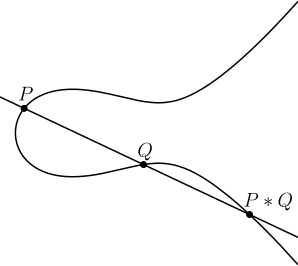
\includegraphics[width=.8\textwidth]{../build_plots/elliptic_curve_addition}
    \end{minipage}%
    \begin{minipage}{.5\textwidth}
        \centering
        \includegraphics[width=.8\textwidth]{../build_plots/elliptic_curve_doubling}
    \end{minipage}
    \vspace{-1em}
    \caption{The composition of points on the elliptic curve $y^2 = x^3 - \frac{3}{2}x + 2$ plotted over $\mathbb A_{\mathbb R}^2$.}
    \label{fig:composition}
\end{figure}


What about the point at infinity on the elliptic curve, i.e., $\mathcal P_\infty = (0:1:0)$, is our definition of composition well-defined at this point?
First, we look at $\mathcal P_\infty * Q$ for any other point $Q$ on the elliptic curve.
The vertical line coming down from $\mathcal P_\infty$, crosses $Q:= (Q_x, Q_y)$ and $(Q_x, -Q_y)$.
Second, a neat consequence of $\mathcal P_\infty$ being a triple root in \eqref{ellipticcurve} is that $\mathcal P_\infty * \mathcal P_\infty = \mathcal P_\infty$.
Having discussed these special cases, we are assured that \defref{def:composition} is indeed well-defined.

There is another nice property of composing points in this way.
Namely, if $E$ is defined over $\mathbb Q$, and $P$ and $Q$ are points in $\mathbb P_{\mathbb Q}^2$, then we have that $P * Q \in \mathbb P_{\mathbb Q}^2$ \cite{third_rational_point}.
So the composition of two rational points is also rational.

Sadly however, the rational points on an elliptic curve under composition do not behave as a group as composition is not associative to start with (see \figref{fig:composition_associative}).
On the bright side, without too much effort, we can define a group operation on the rational points on the elliptic curve.

\begin{figure}[ht]
    \centering
    \vspace{-1em}
    \begin{minipage}{.5\textwidth}
        \centering
        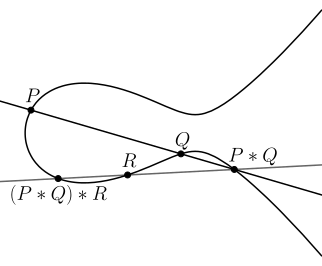
\includegraphics[width=.8\textwidth]{../build_plots/elliptic_curve_composition_1}
    \end{minipage}%
    \begin{minipage}{.5\textwidth}
        \centering
        \includegraphics[width=.8\textwidth]{../build_plots/elliptic_curve_composition_2}
    \end{minipage}
    \vspace{-1em}
    \caption{The composition of points three points $P$, $Q$, and $R$ on the elliptic curve $y^2 = x^3 - \frac{5}{2}x + 2$ plotted over $\mathbb A_{\mathbb R}^2$ in two different ways.}
    \label{fig:composition_associative}
\end{figure}

\begin{definition}\label{plus}
    Take an arbitrary point of the elliptic curve to be the identity element of the group,
    denote it as $\mathcal O$.
    We define the operation $+$ on two points $P$ and $Q$ on the elliptic curve as
    $P + Q = \mathcal O * (P * Q)$.
\end{definition}

Under this operation, the rational points on an elliptic curve form an abelian group.
The proof that this operation is associative can be found in \cite[Section~2.4]{washington}, computer-assisted proofs using the explicit formulas (we derive these in \secref{subsec:addition}) can be found in \cite{associativity_EC} and \cite{associativity_EC_2}.
The following famous theorem gives an important property of this group.

\begin{theorem}[Mordell's theorem, 1922]
    The set of rational points over an elliptic curve is a finitely generated abelian group under the $+$ operator from \defref{plus}.
\end{theorem}
\begin{proof}
    See \cite{mordell}.
\end{proof}
For the set of rational points on an elliptic curve, being finitely generated means that there exists a set of finitely many rational points on the elliptic curve,
such that \textbf{every} other rational point on the curve can be found by repetitively applying our $+$ operation to these points (and reflecting points across the $x$-axis).

We end this subsection by noting something about $\mathcal O$, the identity element of our group.
The choice of $\mathcal O$ is entirely arbitrary, but
in most cases it is chosen to be the point at infinity $(0:1:0)$.
This simplifies things greatly in terms of visualisation and understanding.
Simply draw a line through the two points you want to add,
find the other point of intersection with the elliptic curve and reflect it around
the $x$-axis, and you are done.
This choice also makes sense as it is the only projective point that lies on every elliptic curve.


\subsection{Explicit Formulas for the Group Law}\label{subsec:addition}
Given an elliptic curve over $K$ which, in its affine form, can be written down as
\begin{equation}\label{eq:EC_C}
    y^2 = x^3 + Ax + B.
\end{equation}
We would like to find explicit formulas to add two points $P:=(P_x, P_y)$ and $Q:=(Q_x, Q_y)$ with $P_x,P_y,Q_x,Q_y \in \overline K$ on this elliptic curve,
instead of having to draw lines and finding intersection points.

We take the identity $\mathcal O$ to be $(0:1:0)$ for the remainder of this section (and even this thesis).
Also, for an arbitrary point $R:= (R_x, R_y)$ on the elliptic curve we define $-R:= (R_x, -R_y)$, the point $R$ reflected across the $x$-axis.

There are a couple of cases we can have, we list them below.
\begin{itemize}
    \item[--] \textbf{$P=\mathcal O$ and $Q=\mathcal O$:}
        We have already seen that
        $\mathcal O * \mathcal O = \mathcal O$.
        Hence, we also have
        $\mathcal O + \mathcal O = \mathcal O * (\mathcal O * \mathcal O) = \mathcal O * \mathcal O = \mathcal O$.
    \item[--] \textbf{$P\neq\mathcal O$ and $Q=\mathcal O$:}
        The line through $P$ and $\mathcal O$ is equal to the vertical line through $P$.
        This line intersects $P$ in $-P=(P_x, -P_y)$, the point $P$ reflected across the $x$-axis.
        Thus, $P * \mathcal O = -P$, therefore $\mathcal O + \mathcal P = \mathcal O * (P * \mathcal O) = \mathcal O * (-P) = P$.
    \item[--] \textbf{$P=\mathcal O$ and $Q\neq\mathcal O$:}
        Swap $P$ and $Q$ and apply the case \textbf{$P\neq\mathcal O$ and $Q=\mathcal O$}.
    \item[--] \textbf{$Q = -P\neq\mathcal O$:}
        We find that $P + Q = P + (-P) = \mathcal O * (P * (-P)) = \mathcal O * \mathcal O = \mathcal O$.
        As the line through $P$ and $-P$ will be the vertical line extending to infinity.
    \item[--] \textbf{$P\neq\mathcal O$, $Q\neq\mathcal O$, and $P \neq \pm Q$:}
        We need to find the slope of the lines through
        both $P$ and $Q$, this line will have a slope, $\lambda$, of
        \begin{equation*}
            \lambda = \frac{Q_y-P_y}{Q_x-P_x}.
        \end{equation*}
        Note that we cannot have $Q_x = P_x$ as we assumed that $P\neq \pm Q$.

        The derivation below these cases then finds the explicit coordinates of $P+Q$.
    \item[--] \textbf{$P=Q\neq\mathcal O$ and $P_y \neq 0$:}
        We are trying to find $P+P$, which will be denoted as $[2]P$.
        Note that if $P_y=0$, we enter the case $Q=-P \neq \mathcal O$.
        To do this we need to set up the tangent to the elliptic curve at point $P$.
        Taking the derivative on both sides of the equation $y^2=x^3+Ax+B$, yields $2y\mathrm dy = (3x^2+A)\mathrm dx$.
        The tangent line of the elliptic curve at $P$ will thus have a slope, $\lambda$, of
        \begin{equation*}
            \lambda =
            \left. \frac{\mathrm dy}{\mathrm dx} \right|_{P} =
            \frac{3P_x^2 + A}{2P_y}.
        \end{equation*}
\end{itemize}

Given $\lambda$, the slope of the line through $P$ and $Q$ (which we define the tangent line at $P$ if $P=Q$), we would like to find the third intersection point of the line through $P$ and $Q$ with the elliptic curve.

Define $\mu = P_y - \lambda P_x = Q_y - \lambda Q_x$, then the line through the points $P$ and $Q$ can be written as:
$y = \lambda x + \mu$.
Plugging this formula into \eqref{eq:EC_C} we get:
\begin{equation*}
    y^2 = (\lambda x + \mu)^2 = x^3 + Ax + B.
\end{equation*}
We thus need to find the roots of
\begin{equation*}
    x^3 + Ax + B - (\lambda x + \mu)^2 =
    x^3 - \lambda^2 x^2 + (A - 2\lambda\mu) x + (B - \mu^2)
    .
\end{equation*}
But, we already know two solutions, namely $P_x$ and $Q_x$, since the line goes through these two points.
Define the $x$-coordinate of the third intersection point to be
$x_3$, we now state that
\begin{equation*}
    x^3 - \lambda^2 x^2 + (A - 2\lambda\mu) x + (B - \mu^2) =
    (x-P_x)(x-Q_x)(x-x_3).
\end{equation*}
Writing the right-hand side out gives us
\begin{equation*}
    x^3 - (P_x + Q_x + x_3) x^2 + (P_xQ_x + P_xx_3 + Q_xx_3)x - P_xQ_xx_3.
\end{equation*}
Combining both sides of the equation allows us to equate coefficients that belong to identical degrees of $x$, giving us some direct formulas to calculate $x_3$:
\begin{equation}\label{eq:xcoor_addition}
    x_3 = \lambda^2-P_x-Q_x = \frac{A-2\lambda\mu - P_xQ_x}{P_x + Q_x} = \frac{\mu^2-B}{P_xQ_x}.
\end{equation}
Thus, $P+Q$ can be written as (note the reflection around the $x$-axis)
\begin{equation*}
    P+Q = (\lambda^2-P_x-Q_x, -\lambda(\lambda^2-P_x-Q_x) - \mu).
\end{equation*}

Now, remember that we said that elliptic curves defined over the rational numbers with points $P,Q \in \mathbb P_{\mathbb Q}^2$ on the elliptic curve will have $P*Q \in \mathbb P_{\mathbb Q}^2$.
In other words, the composition of two rational points is also rational.
This result is immediate from the explicit formulas that we derived above.

\begin{examplebox}
    We define an elliptic curve over $\mathbb A_{\mathbb Q}^2$ with the affine form
    \begin{equation}\label{eq:EC_example}
        y^2 = x^3 -2x + 2.
    \end{equation}

    Plugging in $\frac{1}{2}$ and $-\frac{3}{2}$ into the equation of the elliptic curve will result in the two points
    $P=\left(\frac{1}{2}, \sqrt{\frac{1}{2^3} - 1 + 2}\right) = \left( \frac{1}{2}, \frac{3}{\sqrt{8}} \right)$
    and
    $Q=\left(-\frac{3}{2}, -\sqrt{-\frac{3^3}{2^3} + 3 + 2}\right) = \left(-\frac{3}{2}, \sqrt{\frac{13}{8}}\right)$
    on the elliptic curve.
    A visualisation of this addition can be seen in \figref{fig:example_addition}.
    Remember that although the elliptic curve is defined over $\mathbb A_{\mathbb Q}^2$, all points of the elliptic curve reside in $\mathbb P_{\overline{\mathbb Q}}^2$.

    We get line through $P$ and $Q$, in the form as $y=\lambda x + \mu$, with coefficients
    \begin{equation*}
        \lambda = \frac{P_y-Q_y}{P_x-Q_x} = \frac{1}{2} \cdot \frac{3+\sqrt{13}}{2\sqrt{2}}, \quad
        \mu = P_y-\lambda P_x
          = \frac{3}{\sqrt{8}} - \frac{1}{2} \cdot \frac{3+\sqrt{13}}{2\sqrt{2}} \cdot \frac{1}{2}
          = \frac{9 - \sqrt{13}}{8\sqrt{2}}.
    \end{equation*}
    The final addition can be written and simplified to
    \begin{equation*}
        P+Q = \left(\frac{27+3\sqrt{13}}{16}, -\frac{48+7\sqrt{13}}{16\sqrt{2}}\right)
        \approx (2.36, -3.24).
    \end{equation*}
    \begin{figure}[H]
        \centering
        \vspace{-1em}
        \begin{minipage}{.5\textwidth}
            \centering
            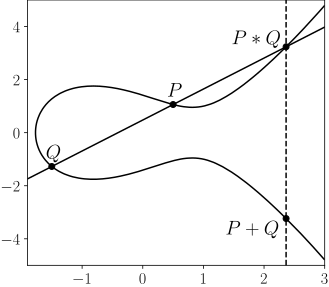
\includegraphics[width=.9\textwidth]{../build_plots/elliptic_curve_example_addition}
        \end{minipage}%
        \begin{minipage}{.5\textwidth}
            \centering
            \includegraphics[width=.9\textwidth]{../build_plots/elliptic_curve_example_doubling}
        \end{minipage}
        \vspace{-1em}
        \caption{Various additions of two points on the elliptic curve from \eqref{eq:EC_example}.}
        \label{fig:example_addition}
    \end{figure}
    \tcbline

    As a different example we will add
    $P=\left(\frac{3}{2}, \sqrt{\frac{3^3}{2^3} - 3 + 2}\right) = \left( \frac{3}{2}, \sqrt{\frac{19}{8}} \right)$
    to itself, using the same elliptic curve from \eqref{eq:EC_example}.
    A visualisation of this addition can be seen in \figref{fig:example_addition}.

    We compute the slope $\lambda$ of the tangent line at $P$ and the parameter $\mu$ such that the tangent line at $P$ can be written as $y = \lambda x + \mu$.
    \begin{equation*}
        \lambda = \frac{3P_x^2 + A}{2P_y} = \frac{\frac{27}{4}-2}{\sqrt{19/2}} = \sqrt{\frac{19}{8}}, \quad
        \mu = P_y-\lambda P_x
          = \sqrt{\frac{19}{8}} -\sqrt{\frac{19}{8}} \cdot \frac{3}{2}
          = -\frac{1}{2} \sqrt{\frac{19}{8}}.
    \end{equation*}
    The final $x$-coordinate of $P+P$ can be evaluated in numerous ways according to \eqref{eq:xcoor_addition}.
    The $y$-coordinate can be calculated using $\lambda ([2]P)_x + \mu$,
    or by plugging the newly found $x$-coordinate in \eqref{eq:EC_example} and taking the positive solution.
    All in all, we get the relations
    \begin{gather*}
        (P+P)_x = ([2]P)_x = \lambda^2 - 2P_x = \frac{\mu^2-B}{P_x^2} = \frac{A - 2\lambda \mu - P_x^2}{2P_x} = -\frac{5}{8}, \\
        (P+P)_y = ([2]P)_y = \lambda ([2]P)_x + \mu = -\sqrt{([2]P)_x^3 - 2 ([2]P)_x + 2} = -\frac{9}{32} \sqrt{38}, \\
        P+P = [2]P = \left(-\frac{5}{8}, -\frac{9}{32}\sqrt{38}\right) \approx (-0.625, -1.734).
    \end{gather*}
\end{examplebox}


\section{Elliptic Curves over Finite Fields}\label{sec:ec_over_ff}
For the remainder of this section, let $q$ be the power of some prime $p$, such that $q=p^m$ for some positive integer $m$.
Extending \defref{hom_curve}, we find that an elliptic curve (in short Weierstrass form) defined over the finite field $\mathbb F_q$ will have coefficients in $\mathbb F_q$.
We note that the formulas for addition over an elliptic curve derived in \secref{subsec:addition} can also be evaluated over $\mathbb F_q$.

\begin{examplebox}
    We define an elliptic curve over the finite field $\mathbb F_7$ with the affine form
    \begin{equation*}
        y^2 = x^3 -2x + 2.
    \end{equation*}
    Using brute force one can find some points on the elliptic curve.
    For example $P=(1, 1)$ and $Q=(4,3)$ are both on the elliptic curve.
    To add $P$ and $Q$ we evaluate (in $\mathbb F_7$)
    \begin{equation*}
        \lambda = \frac{P_y-Q_y}{P_x - Q_x} = \frac{-2}{-3} = \frac{2}{3} = 3, \qquad
        \mu = P_y - \lambda P_x = 1-3 = -2.
    \end{equation*}
    Therefore, $\lambda^2 - P_x - Q_x = 3^2-1-4 = 4$ and $P+Q = (4, -4 \lambda - \mu) = (4, -3\cdot4 + 2) = (4, 4)$.

    Similarly, evaluating $P+P$ gives $\lambda = \frac{3\cdot 1^2-2}{2} = 4$ and $\mu = 1-4=-3$.
    Therefore, $P+P = (0, 3)$.
\end{examplebox}

In general, points of an elliptic curve $E$ defined over a finite field $\mathbb F_q$ are not necessarily contained in the finite field, instead the points belong to $\overline {\mathbb F}_q$, the algebraic closure of $\mathbb F_q$, from \defref{alg_closure}.
\begin{examplebox}
    Take the elliptic curve $E: y^2 = x^3-2x+2$ defined over the finite field $\mathbb F_7$.

    Let $s$ be a root of the polynomial $x^2+6x+3 \in \mathbb F_7[x]$ and define $\mathbb F_{7^2}$ to be $\mathbb F_7[x]/(x^2+6x+3)$ as in \theoref{ff_from_polrings}.
    The $\mathbb F_{7^2}$-rational (but not $\mathbb F_7$-rational) point $P = (2, 6s+4)$ is on the elliptic curve $E$ as $(6s+4)^2 = s^2 + 6s + 2 = 6 = 2^3-2\cdot 2 + 2$.
\end{examplebox}
In this example, we have seen that the points of an elliptic curve over $\mathbb F_q$ are not always $\mathbb F_q$-rational.
We denote the subset of points on $E$ that \textbf{are} $\mathbb F_q$-rational by $E(\mathbb F_q)$.

The security of many cryptosystems relies on the difficulty of the \textit{discrete logarithm problem} in a group $(\mathbb Z/p\mathbb Z)$ for some large prime $p$.
We state it as follows.
Given $\alpha \in (\mathbb Z / p\mathbb Z)$ and $\beta \in \langle \alpha \rangle$ (that is, $\beta$ can be generated by $\alpha$), find any integer $x$ such that $\alpha^x = \beta$

Using our newfound addition of points on elliptic curves we can formulate the \textit{elliptic curve discrete logarithm problem}.
The problem is that given a prime $p$, an elliptic curve $E$ defined over $\mathbb F_p$ and the points $P,Q \in E(\mathbb F_p)$ (assuming that $Q$ is a multiple of $P$), find an integer $m$ so that $[m]P=Q$.
This problem is the basis for elliptic curve cryptography (ECC), an encryption method that has existed for nearly four decades \cite{miller} \cite{koblitz}.

Also, Lenstra Elliptic Curve factorisation \cite[Section~4.4]{silverman} \cite{ecm}, can factor positive integers $n$.
Let $n$ denote a number that is not prime (checking primality is a relatively cheap operation compared to factoring), the algorithm starts by finding an elliptic curve over $\mathbb Z/n\mathbb Z$ and a point $P \in E(\mathbb Z / n \mathbb Z)$.
Now, it will continue to find multiples of the point $P$, until, using the addition formulas from \secref{subsec:addition}, we try to invert a residue class in $\mathbb Z/n \mathbb Z$ that has no inverse (such residue classes exist as $n$ is not prime).
We can then retrieve a factor of $n$ using the residue class that has no inverse in $\mathbb Z/n \mathbb Z$.


\chapter{Morphisms of Elliptic Curves}\label{chap:morphisms}
In order to understand the algorithm that drives CSIDH, we must first take a look at mappings between two elliptic curves called morphisms.

In this chapter we will first look at a special type of morphism of elliptic curves called an isogeny.
Afterwards, we discuss isomorphism classes of elliptic curves.
Intertwining the theory from \chapref{chap:number_fields} allows us to examine the structure of the endomorphism ring of an elliptic curve.
It also allows us to define the action of ideal classes on isomorphism classes of elliptic curves, a concept that gives rise to isogeny graphs, a helpful visualisation for isogeny-based cryptography.

The principles covered in this chapter are crucial to understanding CSIDH, linking all previously discussed theories to provide a thorough background on the algorithm introduced in the next chapter.

\begin{warning}
    Unless stated otherwise, all elliptic curves in this chapter will be defined over the finite field $\mathbb F_p$ with $p > 3$ a prime number.
\end{warning}

\section{Isogenies of Elliptic Curves}\label{sec:isogenies}
Defining an isogeny is typically done using algebraic geometry.
However, we take a more implicit route to avoid some of this theory.
At each step, we try to provide proof that our definitions are equivalent to the definitions using more sophisticated algebraic geometry.
Typical definitions of isogenies can be found in
\cite[Chapter~5,Section~9.6]{galbraith_crypto},
\cite{rational_maps}, and
\cite[Chapters~I,II,Section~III.4]{arithmetic}.


\begin{theorem}\label{Sato-Tate}
    Two elliptic curves $E_1$ and $E_2$ over a finite field $\mathbb F_p$ are \emph{isogenous} over $\mathbb F_p$ if and only if $\#E_1(\mathbb F_p) = \#E_2(\mathbb F_p)$.
\end{theorem}
\begin{proof}
    See \cite{tate_isogeny_theorem}, \cite[Theorem~9.7.4]{galbraith_crypto} (only for sufficiency), or \cite[Exercise~5.4]{arithmetic}.
\end{proof}
\begin{definition}\label{is_isogeny}
    Let $E_1$ and $E_2$ be elliptic curves of the form $y^2 = x^3 + ax^2 + bx + c$ with $a,b,c \in \mathbb F_p$.
    If $E_1$ is isogenous to $E_2$, i.e., $\#E_1(\mathbb F_p) = \#E_2(\mathbb F_p)$, then there exists a map $\phi: E_1 \to E_2$ satisfying $\phi(\mathcal O) = \mathcal O$ called a \textit{non-zero isogeny} from $E_1$ to $E_2$.
    Every \textit{isogeny} is either the \textit{zero isogeny}, mapping each point $P \in E_1$ to $\mathcal O \in E_2$, or a non-zero isogeny between isogenous elliptic curves\footnote[2]{In other literature this is said to be an isogeny defined over $\mathbb F_p$. Since all isogenies in this thesis will be defined over $\mathbb F_p$, we just call them isogenies.}.
    Every non-zero isogeny is can be expressed as a rational map
    \begin{equation}\label{rat_map}
        \phi(x, y) = \left( \frac{f(x)}{k(x)}, \frac{g(x)}{h(x)}y \right),
    \end{equation}
    where $f,k,g,h \in \mathbb F_p[x]$, $\gcd(f, k) = 1$, and $\gcd(g, h) = 1$ (\defref{alg_polrings}).
    A proof of this can be found in \cite[Lemma~4.26]{rational_maps} and \cite[Lemma~9.6.12]{galbraith_crypto}.
    The \textit{kernel} of any isogeny $\phi: E_1 \to E_2$ is denoted as $\ker(\phi)$ and defined as $\ker(\phi) = \{ P \in E_1: \phi(P) = \mathcal O \}$.
\end{definition}
\begin{theorem}\label{ker_pol}
    Let $E_1$ be isogenous to $E_2$ and let $\phi: E_1 \to E_2$ be a non-zero isogeny given by \eqref{rat_map}.
    Then, any point $(x_0:y_0:1) \in E_1$ is in the kernel of $\phi$ if and only if $k(x_0) = 0$
\end{theorem}
\begin{proof}
    This follows directly from \cite[Corollary~4.28]{rational_maps}.
\end{proof}

\begin{definition}
    The \textit{kernel polynomial} of a non-zero isogeny is $k(x) \in \mathbb F_p[x]$ from \eqref{rat_map} divided by its lead coefficient (in order for the kernel polynomial to become a monic polynomial).
    We note that the kernel polynomial is uniquely determined \cite[p.~9]{rational_maps}.
\end{definition}


\begin{examplebox}
    Let $E_1: y^2 = x^3 + 3x^2 + 2x$ and $E_2: y^2 = x^3 + 3 x^2 + 6x+4$ be elliptic curves defined over the finite field $\mathbb F_7$.
    As $\#E_1(\mathbb F_7) = \#E_2(\mathbb F_7)=8$, we know that $E_1$ and $E_2$ are isogenous.
    Therefore, there exists an isogeny $\phi: E_1 \to E_2$ between them.
    In fact, such an isogeny is given by the rational map
    \begin{equation*}
        \phi(x, y) = \left( \frac{x^2+2}{x}, \frac{x^2y - 2y}{x^2} \right).
    \end{equation*}

    Take $P=(4,1) \in E_1$, then $\phi(P) = \left(\frac{18}{4}, \frac{14}{16} \right) = (1, 0)$ and indeed $(1, 0) \in E_2$.
    If we would have taken $P=(0,0) \in E_1$, then $\phi(P) = \mathcal O\in E_2$.
    In fact, one can show that $\ker \phi = \{ \mathcal O, P \}$.

    To show that the isogeny $\phi$ is not one-to-one note that
    both $(3,2)\in E_1$ and $(3,5)\in E_1$ map to $(6,0) \in E_2$.
    Furthermore, no $P \in E_1(\mathbb F_7)$ maps to $(2,1) \in E_2(\mathbb F_7)$.
    However, $P = (6s+5, 4s+2) \in E_1(\mathbb F_{7^2})$, where both the $x$ and the $y$ coordinate of $P$ are elements of $\mathbb F_{7^2} := \mathbb F_7[s]/(s^2+6s+3)$ satisfies
    \begin{align*}
        \phi(6s+5, 4s+2) &= \left( \frac{(6s+5)^2 + 2}{6s+5}, \frac{(6s+5)^2 - 2}{(6s+5)^2} (4s+2) \right) \\
                         &= \left( 6s+5 + 2(4s+2), (1 - 2 (4s+2)^2) (4s+2) \right) \\
                         &= \left( 2, (1 - 2 (4s+5)) (4s+2) \right) \\
                         &= \left( 2, 1 \right)
    \end{align*}
    by the long division from \secref{sec:pol_rings} and the relation $(6s+5)^{-1} = 4s+2$.
\end{examplebox}


\section{Isomorphism Classes of Elliptic Curves}\label{sec:isom_classes}
\begin{definition}
    Let $E_1$ and $E_2$ be elliptic curves defined over $\mathbb F_p$.
    We say that $E_1$ and $E_2$ are \textit{$\mathbb F_p$-isomorphic} if there exist isogenies $\phi_1: E_1 \to E_2$ and $\phi_2: E_2 \to E_1$ such that for every point $P \in E_1$ we have that $\phi_2(\phi_1(P)) = P$, i.e., $\phi_2 \circ \phi_1$ is the identity map.
    The isogenies $\phi_1$ and $\phi_2$ are then called \textit{$\mathbb F_p$-isomorphisms}.
    Define a relation $\cong$ on arbitrary elliptic curves $E_1$ and $E_2$, such that $E_1 \cong E_2$ if and only if $E_1$ and $E_2$ are $\mathbb F_p$-isomorphic (this notation will come back later).
    Then this relation forms an equivalence relation.
    The equivalence classes are called \textit{$\mathbb F_p$-isomorphism classes} of elliptic curves.
\end{definition}


\begin{examplebox}
    Define the elliptic curve $E_1: y^2 = x^3 + 2x + 1$ over $\mathbb F_7$
    and the elliptic curve
    $E_2: y^2 = (x+1)^3 + 2(x+1) + 1 = x^3 + 3x^2 + 5x + 4$ over $\mathbb F_7$.
    These curves are isogenous, so that there exists an isogeny between them.
    In fact, $\phi_1: E_1 \to E_2$ given by $\phi_2(x,y) = (x+1, y)$ and $\phi_2: E_2 \to E_1$ given by $\phi_2(x,y) = (x-1, y)$ are two isogenies.
    We can see that for every point $P \in E_1$ we have that $\phi_2(\phi_1(P)) = P$, proving that $E_1$ and $E_2$ are $\mathbb F_p$-isomorphic, so that $E_1$ and $E_2$ are in the same $\mathbb F_p$-isomorphism class.
\end{examplebox}

Besides $\mathbb F_p$-isomorphisms, there also exist $\overline {\mathbb F}_p$-isomorphisms.
Before we state when two curves are $\overline {\mathbb F}_p$-ismorphic in \theoref{j-isomorphic}, we first look at the $j$-invariant of an elliptic curve.

\begin{definition}\label{j-inv}
    Let $E: y^2 = x^3+ax^2 + bx + c$ be an elliptic curve with $a,b,c \in \mathbb F_p$.
    We define
    $b_2 = 4a$, $b_4 = 2b$, $b_6 = 4c$, and $b_8=\frac{1}{4}(b_2b_6 - b_4^2)$.
    The $j$-invariant of the elliptic curve equals
    $$j(E) = \frac{(b_2^2 - 24b_4)^3}{9b_2b_4b_6-b_2^2 b_8 - 8b_4^3 - 27 b_6^2} \in \mathbb F_p.$$
\end{definition}

\begin{theorem}\label{j-isomorphic}
    Two elliptic curves $E_1$ and $E_2$ are $\overline{\mathbb F}_p$-isomorphic (equivalently, there exists an $\overline{\mathbb F}_p$-isormorphism between them) if and only if their $j$-invariants are equal, that is $j(E_1) = j(E_2)$.
\end{theorem}
\begin{proof}
    A proof of this theorem is listed in \cite[III.1.4(b)]{arithmetic}.
\end{proof}
\begin{theorem}\label{Fp-isomorphic}
    An elliptic curve $E': y^2 = x^3+A'x + B'$ in short Weierstrass form is $\mathbb F_p$-isomorphic to the elliptic curve $E: y^2 = x^3+Ax+B$ if and only if there exists a $u \in \mathbb F_p^*$ such that $A' = u^4A$ and $B' = u^6B$.
    Moreover, two elliptic curves that are $\mathbb F_p$-isomorphic are also $\overline{\mathbb F}_p$-isomorphic, the converse does not hold in general.
\end{theorem}
\begin{proof}
    A proof of this theorem can be found in \cite[Theorems~2.2.2-2.2.4]{isom_class}.
\end{proof}

\begin{examplebox}


    Let $E_1: y^2 = x^3 + 2x + 1$ be an elliptic curve defined over $\mathbb F_5$.
    Similarly, let $E_2: y^2 = x^3+3x+2$ be an elliptic curve defined over $\mathbb F_5$.
    We have that $j(E_1) \equiv j(E_2) \equiv 4 \pmod 5$, so that the exists an $\overline{\mathbb F}_5$-isomorphism between $E_1$ and $E_2$ from \theoref{j-isomorphic}.
    However, they are not isomorphic due to \theoref{Fp-isomorphic} as there does not exist a $u \in \mathbb F_5^*$ such that $3\equiv 2u^4 \pmod 5$ and $2 \equiv u^6 \pmod 5$.
\end{examplebox}


\section{Montgomery Curves}\label{sec:mont_curves}
A \textit{Montgomery curve} is an elliptic curve over a finite field $\mathbb F_p$ with $p>3$, of the form $y^2=x^3+Mx^2+x$ for some $M \in \mathbb F_p$.
Here, $M$ is called the \textit{Montgomery coefficient} of the elliptic curve.
In CSIDH \cite{CSIDH} (which is discussed in \secref{sec:CSIDH}) these curves are extensively used as they make calculations easier.
Moreover, CSIDH only works with $\mathbb F_p$-isomorphism classes that contain exactly one Montgomery curve \cite[p.~5]{CSIDH}; this allows them to denote an entire $\mathbb F_p$-isomorphism class by the Montgomery coefficient of that Montgomery curve.
\begin{examplebox}
    The curve $E: y^2=x^3+2x+1$ defined over $\mathbb F_{11}$ is isomorphic to the curve $y^2 = x^3 + x^2 + x$ in Montgomery form with a Montgomery coefficient of 1.
    CSIDH thus denotes the $\mathbb F_{11}$-isomorphism class containing $E$ by $1$.
\end{examplebox}

An additional use of Montgomery curves for cryptography is that the $x$-coordinate of $[k]P$ for some $k \in \mathbb Z_{>0}$ and point $P$ on the curve can be found significantly faster than for normal elliptic curves \cite[p.~26]{CSIDH}.
This fact is used extensively in CSIDH to speed up computations in their encryption scheme.


\section{The Endomorphism Ring}\label{sec:endomorphism_ring}
In the previous sections we talked about two elliptic curves being isogenous and isomorphic.
In this section we will talk about the mappings that map an elliptic curve to itself.
\begin{definition}
    Let $E$ be an elliptic curve.
    An \textit{$\mathbb F_p$-endomorphism} is an isogeny $\phi$ from $E$ to $E$.
    The set of all endomorphisms of the elliptic curves is called the \textit{$\mathbb F_p$-endomorphism ring} of $E$, and is denoted as $\mathrm{End}_{\mathbb F_p}(E)$.
    Let $\phi$ and $\psi$ denote $\mathbb F_p$-endomorphisms from $E$ to $E$.
    Then the $\mathbb F_p$-endomorphism ring forms a ring under the addition operation $(\phi + \psi)(P) = \phi(P) + \psi(P)$ and the multiplication operation $(\phi\cdot \psi)(P) = \phi(\psi(P))$, where $P$ is any point in $E$ \cite[Proposition~4.2(c)]{arithmetic}.
\end{definition}
\begin{remark}
    In this thesis we will only consider $\mathbb F_p$-endomorphisms, therefore, we will call them endomorphisms from now on.
    We will also define $\mathrm{End}(E) := \mathrm{End}_{\mathbb F_p}(E)$ and call the $\mathbb F_p$-endomorphism ring of $E$ the endomorphism ring of $E$.
\end{remark}

Let $E_1$ and $E_2$ be elliptic curves and let $[m]: E_1 \to E_2$ with $m \in \mathbb Z$ denote the multiplication-by-$m$ map sending each point $P \mapsto [m]P$, i.e., adding each point to itself a total of $m$ times.
We certainly have that the multiplication-by-1 map sends $E_1$ to itself, i.e., $[1]: E_1 \to E_1$ is an endomorphism.
Since $[1] \in \mathrm{End}(E_1)$, we can use the addition operation defined on the endomorphism ring to see that $([1]+[1])(P)=[1]P + [1]P = [2]P$ for any point $P \in E_1$.
Thus, the multiplication-by-2 map, $[2]$, is also an endomorphism.
Likewise, one can show that every multiplication-by-$m$ map is an endomorphism.

\begin{examplebox}
    Let $E: y^2 = x^3 + 2x + 1$ be an elliptic curve
    defined over $\mathbb F_7$.
    The isogeny $\phi: E \to E$ defined by
    $$\phi(x, y) = \left(\frac{x^4-x}{-3x^3-3}, \frac{x^6 - x^3 - 1}{x^6 + 2x^3 + 1} y\right)$$
    is an endomorphism mapping each point $P$ to $[2]P$ by the formulas from \secref{subsec:addition}.
\end{examplebox}


\begin{definition}
    Let $p>3$ be a prime and let $E$ be an elliptic curve over $\mathbb F_p$.
    The $p$th power Frobenius map $\pi: E \to E$ defined by the rational map
    $(x, y) \mapsto (x^p, y^p)$
    is an endomorphism.
    Therefore, we call this map the \textit{$p$th power Frobenius endomorphism} of $E$.
\end{definition}

Let $E$ be an elliptic curve over $\mathbb F_p$.
As we have $x^p = x$ for all $x \in \mathbb F_p$ (\theoref{fermat}), all points in $E(\mathbb F_p)$ are fixed by the $p$th power Frobenius endomorphism.
However, the $p$th power Frobenius endomorphism permutes all points in $E$ that are not in $E(\mathbb F_p)$.


\begin{theorem}\label{all_kernels}
    Let $E$ be an elliptic curve, and let $G$ be a finite subgroup (i.e., a subgroup that is a finite group) of the points on $E$ stable under applying the $p$th power Frobenius endomorphism $\pi$, i.e., for each $P \in G$ we have $\pi(P) \in G$.
    There is a unique elliptic curve $E'$ up to $\mathbb F_p$-isomorphism and an isogeny $\phi: E \to E'$ satisfying $\ker \phi = G$.
\end{theorem}
\begin{proof}
    See Proposition III.4.12 and Exercise 3.13(e) of \cite{arithmetic}.
    Also, see \cite[Theorem~9.6.19]{galbraith_crypto} or \cite[Lemma~6]{CSIDH}.
\end{proof}

\begin{remark}
    For a given curve $E$ and subgroup $G$, Velu \cite{velu} found an algorithm that computes explicit formulas for the curve $E'$ and the rational maps of the isogeny $\phi: E \to E'$.
\end{remark}

\begin{remark}
    Note that the kernel of the $p$th power Frobenius endomorphism is $\{ \mathcal O \}$, a characteristic that it shares with other (purely) inseparable isogenies.
    On the contrary, separable isogenies are characterised by their kernel (not uniquely).
    In following sections we use \theoref{all_kernels} together with Velu's formulas \cite{velu} to convert a non-trivial kernel back into a separable isogeny.
    Although the separable isogeny we retrieve is not unique, our point of interest, the codomain of the isogeny, is unique up to $\mathbb F_p$-isomorphism, which is all we need.
    Therefore, inseparable isogenies are not very relevant to our use case and separability is not discussed formally in this thesis.
    For more information regarding the subject the reader is referred to \cite[Section~II.2]{arithmetic} or \cite[Sections~9.6,9.7]{galbraith_crypto}.
    The fact that the kernel of our isogenies is non-trivial, can be seen from \cite[Corollary~9.7.3]{galbraith_crypto} and \cite[Corollaries~III.5.3-III.5.5]{arithmetic}.
\end{remark}

\begin{definition}
    The \textit{trace} of the $p$th power Frobenius endomorphism $\pi$ of an elliptic curve $E$ is the integer $t$ satisfying $\#E(\mathbb F_p) = p + 1 - t$.
    We often call $t$ the \textit{trace of Frobenius} of $E$.
\end{definition}
\begin{theorem}\label{frobenius_satisfies}
    Let $E$ be an elliptic curve over $\mathbb F_p$.
    The $p$th power Frobenius endomorphism $\pi$ over $E$ satisfies
    $\pi^2 - [t]\pi + [p] = 0$, that is, the composition of these functions is the zero isogeny.
\end{theorem}
\begin{proof}
    See \cite[Theorem~V.2.3.1(b)]{arithmetic}.
\end{proof}

Another way of stating this theorem is that for \textbf{any} point $P$ in $E(\overline {\mathbb F}_p)$ (thus even the ones defined over the algebraic closure of $\mathbb F_p$)
we know that $\pi(\pi(P)) - [t]\pi(P) + [p]P = \mathcal O$ as noted in \cite[p.~6]{ideals_on_curves}.
\begin{examplebox}
    Let $E: y^2 = x^3 + 3x + 2$ be an elliptic curve defined over $\mathbb F_{5}$ and let $\mathbb F_{5^2} := \mathbb F_5[s]/(s^2+4s+2)$.
    Furthermore, we define the point $P=(s+4,s+3) \in E(\mathbb F_{5^2})$.

    For all points $Q := (Q_x, Q_y) \in E(\mathbb F_5)$ we have $\pi(Q) = (Q_x^5, Q_y^5) = Q \in E(\mathbb F_5)$ by Fermat's little theorem (\theoref{fermat}).
    However, for our point $P=(s+4,s+3)\in E(\mathbb F_{5^2})$ we have that $\pi(P) = (4s, 4s+4) \neq P$, and that $\pi(P) = (4s, 4s+4) \in E(\mathbb F_{5^2})$.
    We apply $\pi$ again to give $\pi^2(P):=\pi(\pi(P))$, essentially performing the map $(x, y) \mapsto (x^{5^2}, y^{5^2})$, to find that $\pi^2(P) = (s+4, s+3) = P$.
    In fact, one can show that for any $x \in \mathbb F_{5^2}$ we have that $x^{5^2} \equiv x$, which implies that all points in $E(\mathbb F_{5^2})$ are fixed by applying $\pi^2$.

    Now, \theoref{frobenius_satisfies} states that $\pi^2 - [t]\pi + [5] = 0$ must hold.
    For any point $P \in E(\mathbb F_{5^2})$ we already know that $\pi^2(P) = P$.
    We will verify the equation for our point $P:= (s+4, s+3) \in E(\mathbb F_{5^2})$ by checking whether $\pi(\pi(P)) -[t]\pi(P) + [5]P = \mathcal O$ holds.
    The trace of Frobenius of $E$ equals $1$ as $\#E(\mathbb F_p)=5=5+1-1$.
    Therefore, the equation reduces to checking whether $P - \pi(P) + [5]P = \mathcal O$.
    And indeed $[5+1]P = (4s, 4s+4) = \pi(P)$.
    We have thus shown that \theoref{frobenius_satisfies} holds for our choice of $P \in E(\overline {\mathbb F}_5)$.
\end{examplebox}

\begin{definition}\label{is_supersing}
    An elliptic curve $E$ defined over $\mathbb F_p$ is called \textit{supersingular} if and only if the trace of Frobenius equals 0, otherwise it is called \textit{ordinary} \cite[Theorem~13.4]{supersingular_curves}.
    Furthermore, the trace of Frobenius is preserved under non-zero isogenies by \theoref{Sato-Tate}.
    Therefore, supersingular elliptic curves are never isogenous to ordinary elliptic curves.
\end{definition}

The distinction between supersingular and ordinary elliptic curves is important as CSIDH only uses supersingular elliptic curves in their encryption scheme.

The polynomial $x^2-tx+p \in \mathbb Z[x]$ is called the Frobenius polynomial (remember that $\pi$ satisfies $\pi^2 - [t]\pi + [p] = 0$).
From Hasse's theorem \cite{Hasse} we know that $|t| \leq 2\sqrt{p}$, and therefore $t^2-4p<0$.
Solving the Frobenius polynomial shows that its roots are imaginary numbers.
Those roots can thus \textit{extend} the rationals $\mathbb Q$.
Building on this, we define the number field $K = \mathbb Q(\pi)$, where $\pi$ is a root of the Frobenius polynomial.
Previously we saw that every multiplication-by-$m$ map for $m \in \mathbb Z$ is an endomorphism, likewise, the $p$th power Frobenius endomorphism $\pi$ of an elliptic curve is also an endomorphism.
Thus, we know that the order $\mathbb Z[\pi] \subseteq \mathrm{End}(E)$ for arbitrary elliptic curves $E$ over $\mathbb F_p$.
Using \cite[Theorems~13.6-13.8]{supersingular_curves}, we find that ordinary elliptic curves satisfy $\mathbb Z[\pi]\subseteq \mathrm{End}(E)\subseteq\mathcal O_K$, implying that $\mathrm{End}(E)$ is an order in the number field $K$.

\section{Ideals Acting on Elliptic Curves}\label{ideals_acting}
This section starts by introducing the concept of ideals acting on $\mathbb F_p$-isomorphism classes of elliptic curves; the properties and consequences of these definitions along with their proofs can be found in \secref{ideal_proof}.
A visualisation of the action of ideals on $\mathbb F_p$-isomorphism classes of elliptic curves can be found in \secref{sec:isog_graphs}, which introduces the concept of isogeny graphs.

Choose an elliptic curve $E$ defined over some fixed finite field $\mathbb F_p$ for $p>3$ prime.
Calculate the trace $t$ of the $p$th power Frobenius endomorphism.
Let $\pi$ be a root of the Frobenius polynomial $x^2-tx+p$ and define the imaginary quadratic number field $K = \mathbb Q(\pi)$.

Let $A$ be a subring of $\mathrm{End}(E)$, that is, $A \subseteq \mathrm{End}(E)$.
Then, any $\alpha \in A$ represents an endomorphism of the elliptic curve $E$, thus $\alpha: E \to E$.
Using $\alpha$ we can map every point $P \in E$ to the point $\alpha(P) \in E$.
In particular, if some $\alpha \in A$ can be written in the form $a+b\pi$ for $a,b \in \mathbb Z$, that is, $\alpha=a+b\pi \in \mathbb Z[\pi]$, this sends $P$ to the point $\alpha(P)=(a+b\pi)(P) = [a]P + [b]\pi(P)$.

\begin{definition}\label{action_ideal_curve}
    Let $\mathfrak a$ be a non-zero ideal of $\mathbb Z[\pi]$.
    We define $\mathfrak a E$ to be the $\mathbb F_p$-isomorphism class of elliptic curves determined by the codomain of an isogeny $\phi: E \to \mathfrak aE$ satisfying
    $$\ker \phi = \{ P \in E: \alpha(P) = \mathcal O \text{ for all } \alpha \in \mathfrak a \}.$$
    The existence of such an isogeny where the codomain is unique up to $\mathbb F_p$-isomorphism is guaranteed by \theoref{all_kernels2}.
    Note that $\phi$ maps precisely the points $P$ to the point at infinity which all elements of the ideal $\mathfrak a$ map to the point at infinity.
    In fact, we only need to verify that the generators of $\mathfrak a$ map $P$ to the point at infinity (as the endomorphism ring is a ring).
\end{definition}
As we will see in \lemref{same_class_same_curve}, all ideals in the same ideal class (assuming that $\mathbb Z[\pi] = \mathcal O_K$) give the same $\mathbb F_p$-isomorphism class.
Therefore, instead of speaking of the action of an ideal $\mathfrak a$ on an $\mathbb F_p$-isomorphism class, we often speak of the action of an ideal class on $\mathbb F_p$-isomorphism classes of elliptic curves, denoting $\mathfrak aE$ as $[\mathfrak a]E$.

\begin{examplebox}
    Let $E$ be the elliptic curve $E: y^2 = x^3 + x + 6$ over $\mathbb F_7$.
    Then $\#E(\mathbb F_7) = 11 = 7+1-(-3)$, implying that $t=-3$.
    Our Frobenius polynomial becomes $x^2 + 3x + 7 = 0$.

    Take $K = \mathbb Q(\pi)$ where $\pi$ is the root of $x^2 + 3x + 7$.
    The ideal $(3)$ is inert in $K$ as $x^2+3x+7$ is irreducible in $\mathbb F_3[x]$.

    We want to apply the ideal $\mathfrak a = (3)$ to the elliptic curve $E$ to get $\mathfrak aE$.
    To do this we aspire to find the set $\ker \phi = \{ P \in E: [3]P = \mathcal O \}$ as $3\in\mathfrak a$ generates the ideal $\mathfrak a$.
    The isogeny $\phi$ can be found by evaluating:
    \begin{python}
sage: E = EllipticCurve(GF(7), [1, 6])
sage: E.isogeny(E.scalar_multiplication(3).kernel_polynomial())
    \end{python}
    It turns out that the codomain of this isogeny is the elliptic curve $\mathfrak aE: y^2 = x^3 + 4x + 6$.

    Note that the elliptic curve $\mathfrak aE$ is isomorphic to the elliptic curve $E$ due to \theoref{Fp-isomorphic} with $u=3$.
    Since $\mathcal O_K$ is a principal ideal domain (where only one ideal class exists) and $\mathbb Z[\pi] = \mathcal O_K$ we can see from \lemref{same_class_same_curve} that for all ideals $\mathfrak a$ of $\mathbb Z[\pi]$, the curve $E$ will be $\mathbb F_p$-isomorphic to $\mathfrak aE$ as the ideal classes $[(1)]$ and $[\mathfrak a]$ are identical.

    \tcbline

    Define $E: y^2 = x^3 + x + 3$ over $\mathbb F_7$, the Frobenius polynomial is $x^2 - 2x + 7 = 0$.
    Let $\pi$ be a root of $x^2+2x+7$ (and denote the $p$th power Frobenius endomorphism) and define the order $\mathbb Z[\pi]$ of $\mathbb Q(\pi)$.
    We have that $(2)$ factors in $\mathbb Z[\pi]$ as $(2) = (2, \pi-1)^2 = \mathfrak p_2^2$.
    This example aims to find an elliptic curve $E'$ in the same $\mathbb F_p$-isomorphism class as $\mathfrak p_2 E$.
    To this end, we will compute the intersection of the two sets $S_2 := \{ P \in E: [2]P = \mathcal O \}$ and $S_{\pi-1} := \{ P \in E: \pi(P)-P = \mathcal O \}$ as for the isogeny $\phi: E \to \mathfrak p_2E$ we have that $\ker\phi = S_2 \cap S_{\pi-1}$.

    First, we compute $S_{\pi-1}$, for any $P \in E$ we see that $\pi(P) - P = \mathcal O$ is equivalent to $\pi(P) = P$.
    Since $P$ must be fixed by applying $\pi$, we see that $S_{\pi-1} = E(\mathbb F_p)$.
    Therefore, $\ker\phi = \{ P \in E(\mathbb F_p): [2]P = \mathcal O \}$.
    All points in $\ker \phi$ are thus $\mathbb F_p$-rational and roots of the kernel polynomial of the multiplication-by-2 map (\theoref{ker_pol}).
    Using the following code, we find that the kernel polynomial factors (into irreducible polynomials) as $(x+2)(x^2+5x+5)$.
    \begin{python}
sage: E = EllipticCurve(GF(7), [1, 3])
sage: E.scalar_multiplication(2).kernel_polynomial().factor()
    \end{python}
    Since $x+2 \in \mathbb F_p[x]$ is the only factor of degree 1 (and therefore the only one providing a root in $\mathbb F_p$) we get that the kernel polynomial of $\phi$ is $x+2$.
    And hence $\mathfrak p_2 E$, the codomain of $\phi$, can be found by the following code:
    \begin{python}
sage: E = EllipticCurve(GF(7), [1, 3])
sage: E.isogeny(x+2)
    \end{python}
    Which returns that $E' \cong \mathfrak p_2E: y^2 = x^3 + 6x + 3$.
    The curve $E' \cong\mathfrak p_2E$ is not isomorphic to $E$ as $\mathfrak p_2$ is a non-principal ideal.
\end{examplebox}


\subsection{Properties of Ideals Acting on Elliptic Curves}\label{ideal_proof}
This subsection provides proofs for the action of ideals on elliptic curves.
The goal is to shed light on some properties of this action so that the reader (especially one well versed in group actions) can acquire a better understanding of what is possible with these actions.
Furthermore, this subsection provides a rigorous foundation which is used to define the CSIDH encryption scheme more abstractly in the next chapter.

In the remainder of this subsection we let $E$ denote an elliptic curve defined over a finite field $\mathbb F_p$ for some fixed prime $p>3$.
Also, we let $\pi$ denote the $p$th power Frobenius endomorphism of $E$ as well as the root of the Frobenius polynomial $x^2-tx+p$ and define the number field $\mathbb Q(\pi)$ with the order $\mathbb Z[\pi]$.


\begin{lemma}\label{commute_frobenius}
    Let $E$ and $E'$ denote elliptic curves over $\mathbb F_p$.
    Let $\phi: E \to E'$ be an isogeny sending $E$ to $E'$.
    Let $\pi$ denote the $p$th power Frobenius endomorphism of $E$.
    Similarly, let $\pi'$ denote the $p$th power Frobenius endomorphism of $E'$.
    Then we have $\phi \circ \pi = \pi' \circ \phi$.
\end{lemma}
\begin{proof}
    First, if $\phi$ is the zero isogeny, this equation holds trivially.
    Otherwise, by \defref{is_isogeny}, $\phi$ can be expressed as a rational map
    \begin{equation*}
        \phi(x, y) = \left( \frac{f(x)}{k(x)}, \frac{g(x)}{h(x)}y \right),
    \end{equation*}
    with $f,k,g,h \in \mathbb F_p[x]$.

    By the Freshman's dream \cite[Example~9.42]{freshman}, we have that $f(x^p)=f(x)^p$ for any polynomial $f \in \mathbb F_p[x]$, now, $\phi \circ \pi$ is given by the rational map
    \begin{equation*}
        \phi(x^p, y^p) = \left( \frac{f(x^p)}{k(x^p)}, \frac{g(x^p)}{h(x^p)}y^p \right) = \left( \frac{f(x)^p}{k(x)^p}, \frac{g(x)^p}{h(x)^p}y^p \right).
    \end{equation*}
    which equals the rational map of $\pi' \circ \phi$.
\end{proof}

\begin{theorem}\label{all_kernels2}
    There is a unique elliptic curve $E'$ up to $\mathbb F_p$-isomorphism and an isogeny $\phi: E \to E'$ satisfying $\ker \phi = \{ P \in E: \alpha(P) = \mathcal O \text{ for all } \alpha \in \mathfrak a \}$ for any non-zero ideal $\mathfrak a$ of $\mathbb Z[\pi]$.
\end{theorem}
\begin{proof}
    We need to show that the kernel of the isogeny $\phi$ as defined in \defref{action_ideal_curve} satisfies all conditions of $G$ in \theoref{all_kernels}.
    Let $G$ denote the kernel of $\phi$, we must thus show that $G$ is a finite (follows from the fact that $\mathfrak a$ is non-zero) subgroup of the points on $E$ such that for all $P \in G$ we have that $\pi(P) \in G$, where $\pi$ denotes the $p$th power Frobenius endomorphism.

    First off, let $\alpha$ denote an arbitrary element of a non-zero ideal $\mathfrak a$ of $\mathbb Z[\pi]$.
    Now, $G$ is naturally a subset of the points on $E$.
    Furthermore, $G$ is a subgroup of $E$, since if $P \in G$ and $Q \in G$, then $\alpha(P)=\alpha(Q)=\mathcal O=\alpha(P) + \alpha(Q) = \alpha(P+Q)$, such that $P+Q \in G$, showing that the $+$-operation of $E$ restricts to $G$ (\defref{is_a_group}).
    Next, for all $P \in G$ we have that $\alpha(P) = \mathcal O$, such that $\mathcal O = \alpha(P) = \pi(\alpha(P)) = \alpha(\pi(P))$, giving that $\pi(P) \in G$.
\end{proof}

For any elliptic curve $E'$ isogenous to $E$, we have that $\#E'(\mathbb F_p) = \#E(\mathbb F_p)$ by \theoref{Sato-Tate}.
Therefore, the Frobenius polynomial of $E$ will equal the Frobenius polynomial of $E'$.
Hence, we can not only identify the order $\mathbb Z[\pi]$ as a subring of $\mathrm{End}(E)$ (where $\pi$ denotes the $p$th power Frobenius endomorphism of $E$), but also as a subring of $\mathrm{End}(E')$ (this time $\pi$ denotes the $p$th power Frobenius endomorphism of $E'$).


\begin{theorem}\label{it_commutes}
    Let $\mathfrak a, \mathfrak b \subseteq \mathbb Z[\pi]$ be non-zero ideals.
    Using the notation from \defref{action_ideal_curve} we have that $(\mathfrak a \cdot \mathfrak b)E$, $\mathfrak a (\mathfrak bE)$, and $\mathfrak b (\mathfrak aE)$, all belong to the same $\mathbb F_p$-isomorphism class.
    That is, we can define a left group action where the group of ideals acts on a set of $\mathbb F_p$-isomorphism classes of elliptic curves over $\mathbb F_p$.
\end{theorem}
\begin{proof}
    For any elliptic curve $E'$ isogenous to $E$, and any non-zero ideal $\mathfrak c$ of $\mathbb Z[\pi]$, after identifying $\pi$ with the $p$th power Frobenius endomorphism of $E'$, we get an elliptic curve $\mathfrak cE'$ and an isogeny $\phi_{\mathfrak c}: E' \to \mathfrak cE'$ associated with $\mathfrak c$.
    Also, let the symbol $\forall$ denote ``for all'', we have
    {\allowdisplaybreaks\begin{align*}
        \ker(\phi_\mathfrak a \circ \phi_\mathfrak b)
            &= \{ P \in E: \phi_{\mathfrak a}(\phi_{\mathfrak b}(P)) = \mathcal O \} \\
            &= \{ P \in E: (\alpha \circ \phi_{\mathfrak b})(P) = \mathcal O, \forall \alpha \in \mathfrak a \} \\
            &= \{ P \in E: (\phi_{\mathfrak b} \circ \alpha)(P) = \mathcal O, \forall \alpha \in \mathfrak a \} \\
            &= \{ P \in E: \alpha(P) \in \ker (\phi_\mathfrak b), \forall \alpha \in \mathfrak a \} \\
            &= \{ P \in E: \beta(\alpha(P)) = \mathcal O, \forall \alpha \in \mathfrak a, \forall \beta \in \mathfrak b \} \\
            &= \{ P \in E: (\alpha \cdot \beta)(P) = \mathcal O, \forall \alpha \in \mathfrak a, \forall \beta \in \mathfrak b \} \\
            &= \{ P \in E: \gamma(P) = \mathcal O, \forall \gamma \in (\mathfrak a \cdot \mathfrak b) \} \\
            &= \ker(\phi_{\mathfrak a \cdot \mathfrak b}).
    \end{align*}}Therefore, first applying $\phi_\mathfrak b: E \to \mathfrak bE$ and then $\phi_\mathfrak a: \mathfrak bE \to \mathfrak a(\mathfrak bE)$ is the same as applying $\phi_{\mathfrak a \cdot \mathfrak b}: E \to (\mathfrak a \cdot \mathfrak b)E$.
    For the trivial ideal $(1)$ we know that $(1)E = E$ as it sends all points $P\in E$ to themselves.
    Since $\mathfrak a \cdot \mathfrak b = \mathfrak b \cdot \mathfrak a$, the theorem follows.
\end{proof}

\begin{lemma}\label{acting_principal_ideals}
    Let $\mathfrak a \subseteq \mathbb Z[\pi]$ be a non-zero principal ideal.
    We have $E \cong \mathfrak aE$.
\end{lemma}
\begin{proof}
    Let $\alpha$ denote the generator of the principal ideal $\mathfrak a$, i.e., $\mathfrak a = (\alpha)$.
    Let $\phi: E \to \mathfrak a E$ be the isogeny with kernel $\{ P \in E: \beta(P) = \mathcal O \text{ for all } \beta \in \mathfrak a \}$.
    This kernel is identical to the set $\{ P \in E: \alpha(P) = \mathcal O \}$.
    The endomorphism $\alpha$ has the same kernel as the isogeny $\phi$, proving that the codomain of $\phi$ is $\mathbb F_p$-isomorphic to $E$.
\end{proof}

\begin{lemma}\label{same_class_same_curve}
    Let $\mathfrak a, \mathfrak b \subseteq \mathbb Z[\pi]$ be non-zero ideals.
    If $[\mathfrak a] = [\mathfrak b]$, that is, $\mathfrak a$ and $\mathfrak b$ belong to the same ideal class, we have
    $\mathfrak aE \cong \mathfrak bE$.
\end{lemma}
\begin{proof}
    Assume that there are non-zero $\alpha, \beta \in \mathbb Z[\pi]$ such that $(\alpha)\mathfrak a = (\beta)\mathfrak b$.
    For arbitrary elliptic curves $E$ we then have that
    $((\alpha)\mathfrak a) E \cong ((\beta)\mathfrak b) E$.
    From \theoref{it_commutes} we deduce that
    $(\alpha)(\mathfrak a E) \cong (\beta)(\mathfrak b E)$ must hold.
    Now \lemref{acting_principal_ideals} gives that $\mathfrak aE \cong \mathfrak bE$.

    It rests us to prove our original assumption.
    First assume that it is false, thus, for any non-zero $\alpha, \beta \in \mathbb Z[\pi]$ we never have $(\alpha)\mathfrak a = (\beta)\mathfrak b$.
    In that case $[(\alpha) \mathfrak a] \neq [(\beta) \mathfrak b]$, which would imply that $[(\alpha)] + [\mathfrak a] \neq [(\beta)] + [\mathfrak b]$ and consequently $[\mathfrak a] \neq [\mathfrak b]$, which is a contradiction.
\end{proof}

\begin{theorem}\label{ideal_classes}
    The action of the group of ideal classes $\mathrm{Cl}(\mathbb Z[\pi])$ on a set of $\mathbb F_p$-isomorphism classes of elliptic curves over $\mathbb F_p$ is a group action.
    Therefore, principal ideals $\mathfrak a$ of $\mathbb Z[\pi]$ satisfy $[\mathfrak a]E \cong E$, and we have that $[\mathfrak a \cdot \mathfrak b]E \cong [\mathfrak a] ([\mathfrak b]E) \cong [\mathfrak b]([\mathfrak a] E)$ holds for arbitrary non-zero ideals $\mathfrak a, \mathfrak b$ of $\mathbb Z[\pi]$.
\end{theorem}
\begin{proof}
    From \lemref{acting_principal_ideals} we already know that the identity element of $\mathrm {Cl}(\mathbb Z[\pi])$, the set of principal ideals, acts on $E$ in a similar fashion as the ideal $(1)$ does, namely trivially.
    From \theoref{it_commutes} and \lemref{same_class_same_curve} we deduce that
    $[\mathfrak a \cdot \mathfrak b]E \cong [\mathfrak a] ([\mathfrak b]E) \cong [\mathfrak b]([\mathfrak a] E)$.
    Therefore, $\mathrm {Cl}(\mathbb Z[\pi])$ indeed defines a group action on a set of isomorphism classes of elliptic curves defined over $\mathbb F_p$.
\end{proof}


Remember that for supersingular elliptic curves over $\mathbb F_p$ (which we defined in \defref{is_supersing}) the trace of Frobenius equals $0$ (as long as $p>3$ is prime).
Therefore, the Frobenius polynomial of such an elliptic curve is of the form $x^2+p\in\mathbb Z[x]$ and $\mathbb Z[\pi] = \mathbb Z[\sqrt{-p}]$.

In the special case of $\mathbb F_p$-isomorphism classes of supersingular elliptic curves defined over $\mathbb F_p$ with $p \equiv 1 \pmod 4$, \theoref{ideal_classes} translates to a free and transitive \cite[Definitions~3.6,3.8]{free_transitive} group action.
That is, for two supersingular elliptic curves $E_1, E_2$ there exists an ideal $\mathfrak a$ such that $[\mathfrak a]E_1\cong E_2$, which implies transitivity, and if $[\mathfrak a]E_1 \cong E_1$ then the ideal class $[\mathfrak a]$ must be trivial, which implies that the action must be free.
In other words, the action of $\mathrm{Cl}(\mathbb Q(\sqrt{-p}))$ on the set of isomorphism classes of all supersingular curves defined over $\mathbb F_p$ is free and transitive.
This fact, along with its proof, can be found in \cite[Theorem~7]{CSIDH}.


\subsection{Isogeny Graphs}\label{sec:isog_graphs}
Isogeny graphs help with visualising the effect of applying ideals to elliptic curves.
In this subsection we will briefly look at an example of an isogeny graph and describe what it signifies.

For this example, we will look at elliptic curves defined over $\mathbb F_{59}$.
For any $A \in \mathbb F_{59}$, let the curve $E_A$ denote the elliptic curve with Montgomery coefficient $A$, i.e., $E_A: y^2 = x^3 + Ax^2 + x$.
We will look at the isogeny graph that results from applying the ideals over 3 and 5 repetitively to the starting curve $E_0: y^2 = x^3 + x$, see \figref{isog_graph}.

\begin{figure}[!htb]
    \hspace{-.04\textwidth}%
    \begin{minipage}{.7\textwidth}
        \centering
        \begin{tikzpicture}[ec/.style={ellipse,draw},scale=\textwidth/9cm]
            \draw (90: 3cm) node[ec](0){$E_0$};
            \draw (90-360/9: 3cm) node[ec](29){$E_{29}$};
            \draw (90-2*360/9: 3cm) node[ec](31){$E_{31}$};
            \draw (90-3*360/9: 3cm) node[ec](53){$E_{53}$};
            \draw (90-4*360/9: 3cm) node[ec](11){$E_{11}$};
            \draw (90-5*360/9: 3cm) node[ec](48){$E_{48}$};
            \draw (90-6*360/9: 3cm) node[ec](6){$E_6$};
            \draw (90-7*360/9: 3cm) node[ec](28){$E_{28}$};
            \draw (90-8*360/9: 3cm) node[ec](30){$E_{30}$};
            \begin{scope}[bend left=20, nd/.style={sloped, scale=.8, fill=white}]
                \path[->] (0)  edge node[nd] {$[\mathfrak p_3]$} (29);
                \path[->] (29) edge node[nd] {$[\mathfrak p_3]$} (31);
                \path[->] (31) edge node[nd] {$[\mathfrak p_3]$} (53);
                \path[->] (53) edge node[nd] {$[\mathfrak p_3]$} (11);
                \path[->] (11) edge node[nd] {$[\mathfrak p_3]$} (48);
                \path[->] (48) edge node[nd] {$[\mathfrak p_3]$} (6);
                \path[->] (6)  edge node[nd] {$[\mathfrak p_3]$} (28);
                \path[->] (28) edge node[nd] {$[\mathfrak p_3]$} (30);
                \path[->] (30) edge node[nd] {$[\mathfrak p_3]$} (0);
            \end{scope}

            \begin{scope}[bend left=20, nd/.style={sloped, scale=.8, fill=white}, darkgray]
                \path[->] (29) edge node[nd] {$[\mathfrak q_3]$} (0);
                \path[->] (31) edge node[nd] {$[\mathfrak q_3]$} (29);
                \path[->] (53) edge node[nd] {$[\mathfrak q_3]$} (31);
                \path[->] (11) edge node[nd] {$[\mathfrak q_3]$} (53);
                \path[->] (48) edge node[nd] {$[\mathfrak q_3]$} (11);
                \path[->] (6)  edge node[nd] {$[\mathfrak q_3]$} (48);
                \path[->] (28) edge node[nd] {$[\mathfrak q_3]$} (6);
                \path[->] (30) edge node[nd] {$[\mathfrak q_3]$} (28);
                \path[->] (0)  edge node[nd] {$[\mathfrak q_3]$} (30);
            \end{scope}

            \begin{scope}[bend left=30, nd/.style={sloped, scale=.6, fill=white, pos=.15}]
                \path[->] (0)  edge node[nd] {$[\mathfrak p_5]$} (48);
                \path[->] (48) edge node[nd] {$[\mathfrak p_5]$} (29);
                \path[->] (29) edge node[nd] {$[\mathfrak p_5]$} (6);
                \path[->] (6)  edge node[nd] {$[\mathfrak p_5]$} (31);
                \path[->] (31) edge node[nd] {$[\mathfrak p_5]$} (28);
                \path[->] (28) edge node[nd] {$[\mathfrak p_5]$} (53);
                \path[->] (53) edge node[nd] {$[\mathfrak p_5]$} (30);
                \path[->] (30) edge node[nd] {$[\mathfrak p_5]$} (11);
                \path[->] (11) edge node[nd] {$[\mathfrak p_5]$} (0);
            \end{scope}

            \begin{scope}[bend right=20, nd/.style={sloped, scale=.6, fill=white, pos=.15}, darkgray]
                \path[->] (48) edge node[nd] {$[\mathfrak q_5]$} (0);
                \path[->] (29) edge node[nd] {$[\mathfrak q_5]$} (48);
                \path[->] (6)  edge node[nd] {$[\mathfrak q_5]$} (29);
                \path[->] (31) edge node[nd] {$[\mathfrak q_5]$} (6);
                \path[->] (28) edge node[nd] {$[\mathfrak q_5]$} (31);
                \path[->] (53) edge node[nd] {$[\mathfrak q_5]$} (28);
                \path[->] (30) edge node[nd] {$[\mathfrak q_5]$} (53);
                \path[->] (11) edge node[nd] {$[\mathfrak q_5]$} (30);
                \path[->] (0)  edge node[nd] {$[\mathfrak q_5]$} (11);
            \end{scope}
        \end{tikzpicture}
    \end{minipage}%
    \hspace{-.09\textwidth}%
    \begin{minipage}{.43\textwidth}
        \centering
        \begin{tikzpicture}[ec/.style={},scale=\textwidth/3cm]
            \draw (90: 1) node[ec](0){$E_0$};
            \draw (90-360/9: 1) node[ec](29){$E_{29}$};
            \draw (90-2*360/9: 1) node[ec](31){$E_{31}$};
            \draw (90-3*360/9: 1) node[ec](53){$E_{53}$};
            \draw (90-4*360/9: 1) node[ec](11){$E_{11}$};
            \draw (90-5*360/9: 1) node[ec](48){$E_{48}$};
            \draw (90-6*360/9: 1) node[ec](6){$E_6$};
            \draw (90-7*360/9: 1) node[ec](28){$E_{28}$};
            \draw (90-8*360/9: 1) node[ec](30){$E_{30}$};

            \begin{scope}[bend left=10, blue]
                \path (0)  edge (29);
                \path (29) edge (31);
                \path (31) edge (53);
                \path (53) edge (11);
                \path (11) edge (48);
                \path (48) edge (6);
                \path (6)  edge (28);
                \path (28) edge (30);
                \path (30) edge (0);
            \end{scope}

            \begin{scope}[bend left=30, red]
                \path (0)  edge (48);
                \path (48) edge (29);
                \path (29) edge (6);
                \path (6)  edge (31);
                \path (31) edge (28);
                \path (28) edge (53);
                \path (53) edge (30);
                \path (30) edge (11);
                \path (11) edge (0);
            \end{scope}
        \end{tikzpicture}
    \end{minipage}%
    \vspace{-.9em}
    \caption{
        Isogeny graphs with starting curve defined by $E_0: y^2 = x^3 + x$ over $\mathbb F_{59}$.
        Nodes in the isogeny graph represent $\mathbb F_{59}$-isomorphism classes of supersingular elliptic curves, denoted by the unique Montgomery curve contained in the class.
        Edges in the graph represent isogenies defined by the actions of the ideals over $\{ \textcolor{blue}{3}, \textcolor{red}{5} \}$.
        The figure on the left-hand side gives a complete overview of the mappings that some ideals perform.
        The figure on the right-hand side is a simplified version, merging directional edges of each ideal with its conjugate.
    }
    \label{isog_graph}
\end{figure}

Note that the Frobenius polynomial of $E_0$, which is supersingular, equals $x^2 + 59$.
Therefore, we define $K = \mathbb Q(\sqrt{-59})$.
Let $\alpha = \sqrt{-59}$, and define the order $R = \mathbb Z[\alpha]$ of $K$.
Then, $(3)$ factors in $R$ as $(3, \alpha-1)(3, \alpha+1) = \mathfrak p_3 \mathfrak q_3$
and $(5) = (5, \alpha-1)(5, \alpha+1) = \mathfrak p_5 \mathfrak q_5$.

\begin{remark}
    After applying an ideal to an elliptic curve $E$ defined over $\mathbb F_q$, the Frobenius polynomial does not change.
    This is due to the fact that applying an ideal corresponds to an isogeny and \theoref{Sato-Tate} states that the resulting curve $E'$ satisfies $\#E(\mathbb F_q) = \#E'(\mathbb F_q)$, which gives the same trace of Frobenius.
\end{remark}

As an example, applying the ideal $\mathfrak p_3$ to $E_0$ gives a curve isomorphic to $E_{29}$, i.e., $[\mathfrak p_3]E_0 = E_{29}$.
Applying $\mathfrak p_3$ to $E_{29}$ gives $E_{31}$, and so on until we get back to the original curve $E_0$. A more detailed view is given in \figref{isog_graph}.

\chapter{Encryption Schemes}
In today's world, secure communication has become paramount, with privacy concerns escalating.
This chapter starts by delving into the concept of key exchange (in particular Diffie-Hellman Key Exchange) and how it enables two parties to establish a shared secret.
Building on this foundation, we set the stage for understanding the intricacies of the CSIDH algorithm, the culmination of this thesis.
Elaborating on this algorithm, we present a variant of CSIDH in \secref{gen_CSIDH}, aimed at sparking further exploration and research in this area of cryptography.

\section{Diffie-Hellman Key Exchange}\label{sec:diffie_hellman}
Suppose Alice and Bob, two people living on different sides of the Earth, want to share sensitive information with each other.
Ideally, they wish to send each other messages containing this information securely.
However, Eve can intercept and read the contents of that message.
This is something that Alice and Bob want to avoid.
The Diffie-Hellman key exchange describes how, even if all messages get intercepted, only Alice and Bob are able to read its contents.

First of all, Alice and Bob need to agree on the algorithm they are going to use, an example of applying such an algorithm is listed below.
Once they have done this, they can agree on initialisers of the algorithm called the \textit{public parameters} of the key exchange.
Alice then computes a \textit{private key} that she keeps to herself, which Bob does as well.
Combining public parameters and private key, the algorithm provides a \textit{public key} that Alice sends (via public communication channels) to Bob.
Bob also uses his private key and the algorithm to send a public key to Alice.
Alice receives Bob's public key and Bob receives Alice's public key.
The second stage of the algorithm now uses this public key in combination with their own private key to get to a \textit{shared secret}.
Shared secrets are useful, since \textbf{only} Alice and Bob know this secret, even if all messages get intercepted.
Alice and Bob can use this shared secret to encrypt their sensitive data, which, as long as the shared secret stays a secret to interceptors, can only be read by Alice and Bob.

\begin{figure}[ht]
    \begin{center}
    \begin{tikzpicture}[block/.style={align=center,rectangle,draw}]
        \node [block,line width=.8pt] (1) at (0.0,0.0) {Suppose Alice wants to establish a shared secret with Bob,\\to do this she initiates the Diffie-Hellman Key Exchange.};
        \node [block] (A) at (-3.0,-0.9) {\textbf{Alice}};
        \node [block] (B) at (3.0,-0.9) {\textbf{Bob}};
        \node [block] (A1) at (-3.0,-2.0) {``I'll use the Finite Field\\Diffie-Hellman scheme with\\$p=81233$ and $g=(3 \bmod p)$.''};
        \node [block] (Ask) at (-3.0,-3.3) {Randomly generates a \textit{private key}\\ $a=75629$};
        \node [block] (Bsk) at (3.0,-3.3) {Randomly generates a \textit{private key}\\ $b=26921$};
        \node [block] (Ac) at (-3.0,-4.4) {Computes her \textit{public key}\\$A:=g^a=(21836 \bmod p)$};
        \node [block] (Bc) at (3.0,-4.4) {Computes his \textit{public key}\\$B:=g^b=(63093 \bmod p)$};
        \node [block] (Apk) at (-3.0,-5.3) {``$A=(21836 \bmod p)$''};
        \node [block] (Bpk) at (3.0,-5.8) {``$B=(63093 \bmod p)$''};
        \node [block] (As) at (-3.0,-6.7) {Computes the \textit{shared secret}\\$S:=B^a=(55014 \bmod p)$};
        \node [block] (Bs) at (3.0,-6.7) {Computes the \textit{shared secret}\\$S:=A^b=(55014 \bmod p)$};
        \node [block,line width=.8pt] (2) at (0.0,-8.2) {Alice uses the shared secret $S=(55014 \bmod p)$ to encrypt the message she wants to send\\(e.g., using AES). Afterwards, she sends the encrypted message to Bob. As he also computes\\$S=(55014 \bmod p)$, he can decrypt the message.};
        \draw (A) -- (A1);
        \draw (A1) -- (Ask);
        \path[-{Stealth[length=3mm]}] (A1) edge node[above=-1pt,scale=.9] {\textit{public parameters}} (3.0,-2.0);
        \draw (B) -- (Bsk);
        \draw (Ask) -- (Ac);
        \draw (Bsk) -- (Bc);
        \draw (Ac) -- (Apk);
        \draw (Bc) -- (Bpk);
        \draw (Apk) -- (As);
        \draw (Bpk) -- (Bs);
        \draw[-{Stealth[length=3mm]}] (Apk) -- (3.0,-5.3);
        \path[-{Stealth[length=3mm]}] (Bpk) edge node[above=-1pt,pos=.3] {\textit{public keys}} (-3.0,-5.8);
    \end{tikzpicture}
    \end{center}
    \vspace{-1.5em}
    \caption{An overview of the Diffie-Hellman Key Exchange from \nameref{key_exch_example}.
    Here, an arrow represents sending data across a (public) channel.}
    \vspace{-.5em}
    \label{key_exchange}
\end{figure}

\begin{examplebox}[label={key_exch_example}, nameref={the example}]
    Suppose Alice and Bob want to exchange sensitive information with each other.
    To this end, they want to establish a shared secret.
    See \figref{key_exchange}.

    Alice and Bob create a public channel on which they can send messages.
    On it, they agree to use the Finite Field Diffie-Hellman algorithm to reach a shared secret.
    To set up their system they agree that they will use the modulus $p=81233$ and the base $g=(3 \bmod p) \in \mathbb F_p$ (nowadays, $p$ is typically chosen to be around $2^{3200}$ \cite{keysizes}).

    Now Alice creates a random private key, which must be an integer $< 81233$ according to the algorithm.
    She chooses $a=75629$.
    Likewise Bob generates the private key $b=26921$.

    Following the algorithm they compute their public using their private key,
    Alice computes $A:= g^a = (21836 \bmod p)$. Bob computes $B:= g^b = (63093 \bmod p)$.

    At this point, Eve, who intercepted all their messages, only knows which algorithm Alice and Bob use, together with initialisers $p=81233$ and $g=(3 \bmod p)$.

    Bob now sends his result $B$ to Alice and Alice sends $A$ to Bob.

    Eve is happy, she intercepts the message and knows that $A = (21836 \bmod p)$ and $B = (63093 \bmod p)$.
    However, she remains oblivious to the values of $a$ and $b$ which are presumed to be difficult to figure out (if $p$ were a much larger prime) by herself.

    According to the algorithm Alice now computes $S_a := B^a = (55014 \bmod p)$.
    Bob computes $S_b := A^b = (55014 \bmod p)$.
    We know that $S_a = S_b$ holds as $(g^a)^b = (g^b)^a$ for $a$ and $b$ integers and $g \in \mathbb F_p$.
    Thus, Alice and Bob have a shared secret $S = (55014 \bmod p)$.

    Eve knows that $A=(21836 \bmod p)$ and that $B=(63093 \bmod p)$, but if $p$ were a much larger prime it would be difficult to find the shared secret $S$ without the private keys $a$ or $b$.

    Now, Alice can use the shared secret $S=(55014 \bmod p)$ and a different encryption scheme like poly-alphabetic substitution or AES encryption to encrypt her message.
    She can then send the encrypted message to Bob.
    He can then decrypt the message by using the shared secret.
\end{examplebox}

To develop a new encryption scheme for the Diffie-Hellman key exchange protocol one must first specify how to generate its public parameters and private keys.
The first algorithm of the encryption scheme is then applied to the public parameters and private keys to compute the public keys.
The computed public key is then exchanged with the other person.
Upon receiving the key, the person uses it as an input for the second stage of the algorithm which finds a shared secret.
If a shared secret is obtained the encryption scheme is finalised.

Depending on the strength of the encryption the shared secret is difficult or extremely difficult for an eavesdropper/interceptor Eve to figure out.
The strength of certain encryption schemes is not discussed further in this thesis.


\section{CSIDH}\label{sec:CSIDH}
This section describes CSIDH \cite{CSIDH} and their encryption scheme.
In \tabref{shared_secrets} a small example of the encryption scheme is worked out.
\begin{cryptobox}[label={CSIDH_encryption}, nameref={CSIDH encryption scheme}]
    \textbf{Initialisation.} To start, a prime of the form $p=4\ell_1 \cdot \ell_2 \cdots \ell_n - 1$ is needed
    where $\ell_i$ are small distinct odd primes and $n \in \mathbb Z_{\geq 1}$.
    CSIDH used a $512$-bit prime $p$ \cite[Section~8.1]{CSIDH}, i.e., a prime $p$ satisfying $2^{511} \leq p < 2^{512}$.
    This prime is a public parameter of the encryption scheme.
    We also define the starting curve to be the (supersingular) elliptic curve $E_0: y^2 = x^3 + x$ over $\mathbb F_p$ and define the order $R = \mathbb Z[\pi]$ of $\mathbb Q(\pi)$ obtained by adjoining a root $\pi$ of $x^2+p$ to $\mathbb Q$.

    \textbf{Private Key Generation.}
    The private key is an $n$-tuple $(e_1, \dots, e_n)$ of integers representing exponents, each sampled randomly from a range $\{ -m, \dots, m \}$
    where $2m+1 \geq \sqrt[n]{\#\mathrm{Cl}(R)}$.

    As $x^2 + p = x^2 - 1 = (x-1)(x+1)$ in $\mathbb F_{\ell_i}[x]$ we get that $(\ell_i)$ factors in $R$ as $\mathfrak l_i \overline{\mathfrak l_i}$ where $\mathfrak l_i := (\ell_i, \pi-1)$ and $\overline{\mathfrak l_i} := (\ell_i, \pi+1)$.

    Using the $n$-tuple we define the ideal class $[\mathfrak a] = [\mathfrak l_1^{e_1} \cdots \mathfrak l_n^{e_n}] \in \mathrm{Cl}(R)$, where $[\mathfrak l_i^{-1}] := [\overline{\mathfrak l_i}]$.

    Now, Alice generates a private key and applies $[\mathfrak a]$ to the starting curve $E_0$ and finds an $\mathbb F_p$-isomorphism class containing the Montgomery curve (\secref{sec:mont_curves}) equal to
    $E_A = [\mathfrak a] E_0: y^2 = x^3 + A x^2 + x$ for some $A \in \mathbb F_p$.
    Bob does the same by generating a private key and applying its respective ideal class to the starting curve, obtaining a different curve $E_B$.
    At this point Alice and Bob send their values of $A$ and $B$ to each other over a public channel.

    \textbf{Computing the Shared Secret.}
    Now Alice computes $E_{S_A} := [\mathfrak a]E_B$ and Bob computes $E_{S_B} := [\mathfrak b] E_A$.
    Applying ideal classes is commutative (as can be seen in \figref{isog_graph} and from \theoref{it_commutes} or \theoref{ideal_classes}).
    Thus, we in fact have $E_S := E_{S_A} = E_{S_B}$.
    Hence, Alice and Bob share a secret $S$ determined by the elliptic curve $E_S = [\mathfrak a][\mathfrak b] E_0 = [\mathfrak b][\mathfrak a] E_0: y^2 = x^3 + Sx^2 + x$.
\end{cryptobox}

\begin{table}[ht]
    \begin{center}
        \setlength\tabcolsep{4pt}
        \begin{tabular}{|c|c||c|c|c|c|c|c|c|c|c|}
            \cline{3-11}
            \multicolumn{1}{c}{} & & \multicolumn{9}{|c|}{Some Possible Actions $[\mathfrak a]$} \\
            \cline{3-11}
            \multicolumn{1}{c}{} & & $0$ & $[\mathfrak l_3]$ & $[\mathfrak l_3^2]$ & $[\mathfrak l_3^3]$ & $[\mathfrak l_3^4]$ & $[\mathfrak l_3^5]$ & $[\mathfrak l_3^6]$ & $[\mathfrak l_3^7]$ & $[\mathfrak l_3^8]$ \\
            \multicolumn{1}{c}{} & & $0$ & $[\mathfrak l_5^2]$ & $[\mathfrak l_5^4]$ & $[\mathfrak l_5^6]$ & $[\mathfrak l_5^8]$ & $[\mathfrak l_5]$ & $[\mathfrak l_5^3]$ & $[\mathfrak l_5^5]$ & $[\mathfrak l_5^7]$ \\
            \multicolumn{1}{c}{} & & $[\overline{\mathfrak l_3}\mathfrak l_5^2]$ & $[\mathfrak l_3^4 \mathfrak l_5^3]$ & $[\mathfrak l_3 \mathfrak l_5]$ & $[\overline{\mathfrak l_3^2} \mathfrak l_5]$ & $[\mathfrak l_3^3\mathfrak l_5^2]$ & $[\overline{\mathfrak l_3} \mathfrak l_5^3]$ & $[\mathfrak l_3\mathfrak l_5]$ & $[\mathfrak l_3^2 \mathfrak l_5]$ & $[\mathfrak l_3^2 \mathfrak l_5^3]$ \\
            \cline{3-11}
            \multicolumn{1}{c}{} & & \multicolumn{9}{|c|}{Alice's Resulting Montgomery Coefficient $A$} \\
            \cline{3-11}
            \multicolumn{1}{c}{} & & 0 & 29 & 31 & 53 & 11 & 48 & 6 & 28 & 30 \\
            \hline
            \hline
            \parbox[t]{3mm}{\multirow{9}{*}{\rotatebox[origin=c]{90}{Bob's Coefficient $B$}}} & 0 & 0 & 29 & 31 & 53 & 11 & 48 & 6 & 28 & 30 \\
            & 29 & 29 & 31 & 53 & 11 & 48 & 6 & 28 & 30 & 0 \\
            & 31 & 31 & 53 & 11 & 48 & 6 & 28 & 30 & 0 & 29 \\
            & 53 & 53 & 11 & 48 & 6 & 28 & 30 & 0 & 29 & 31 \\
            & 11 & 11 & 48 & 6 & 28 & 30 & 0 & 29 & 31 & 53 \\
            & 48 & 48 & 6 & 28 & 30 & 0 & 29 & 31 & 53 & 11 \\
            & 6 & 6 & 28 & 30 & 0 & 29 & 31 & 53 & 11 & 48 \\
            & 28 & 28 & 30 & 0 & 29 & 31 & 53 & 11 & 48 & 6 \\
            & 30 & 30 & 0 & 29 & 31 & 53 & 11 & 48 & 6 & 28 \\
            \hline
        \end{tabular}
    \end{center}
    \vspace{-1em}
    \caption{Table of shared secrets with $p=59 = 4\cdot 3 \cdot 5 - 1$. One can use \figref{isog_graph} to verify this table.}
    \label{shared_secrets}
\end{table}

\begin{examplebox}
    Let $\ell_1$ through $\ell_{11}$ denote the first 11 odd primes (thus the primes from 3 to 37).
    Then $p := -1 + 4\prod_{i=1}^{11} \ell_i = 14841476269619$.
    Define the starting curve $E_0: y^2 = x^3+x$ over $\mathbb F_p$.
    We know that the Frobenius polynomial of $E_0$ equals $\pi^2 + p$, thus we define $K = \mathbb Q(\sqrt{-p})$ and the order $R = \mathbb Z[\sqrt{-p}]$.

    Evaluating\footnote{Only a single SageMath shell should be opened as some commands we present rely on earlier definitions.}
    \begin{python}
sage: p = 4*3*5*7*11*13*17*19*23*29*31*37-1
sage: E0 = EllipticCurve(GF(p), [1, 0])
sage: K.<pi> = NumberField(E0.frobenius_polynomial())
sage: K.order(pi).class_number()
    \end{python}
    gives that $\#\mathrm{Cl}(R) = 7617567$.
    Hence, the isogeny graph that we are working on will have at most $7617567$ nodes by \theoref{ideal_classes} (in fact, it has exactly that many nodes).

    Moving on with the encryption scheme,
    we must thus choose a positive integer $m$ such that $2m+1 \geq \sqrt[11]{7617567} \approx 4.223$, we take $m=2$.

    Now, Alice generates a private key by choosing $n=11$ random integers in the range $\{-2, -1, 0, 1, 2\}$.
    Let us say that she generates the tuple $(1,0,0,0,-2,2,0,0,-2,1,0)$.
    She now has to compute $[\mathfrak a]E_0 = [\mathfrak l_1^{e_1} \cdots \mathfrak l_{11}^{e_{11}}]E_0$.
    Note that in this case
    \begin{equation*}
        \mathfrak a = \mathfrak l_1 \cdot \overline{\mathfrak l_5}^2 \cdot \mathfrak l_6^2 \cdot \overline{\mathfrak l_9}^2 \cdot \mathfrak l_{10} = (3, \pi-1)\cdot (13, \pi+1)^2 \cdot (17, \pi-1)^2 \cdot (29, \pi+1)^2 \cdot (31, \pi-1).
    \end{equation*}
    As an example, we will calculate $[\mathfrak l_1]E_0 = [(3, \pi-1)]E_0$.

    From \secref{ideals_acting} we know that the action of the ideal $\mathfrak l_1 = (3, \pi-1)$ is determined by an isogeny $\phi: E \to \mathfrak l_1E$ satisfying
    $\ker\phi = \{ P \in E: [3]P = \mathcal O \} \cap \{ P \in E: \pi(P)-P = \mathcal O \}$.
    Now, if $\pi(P) - P = \mathcal O$, then we will have that $\pi(P)=P$, and we know that $\pi$ only fixes the points $E(\mathbb F_p)$ on the elliptic curve.
    Hence, $\ker \phi = E(\mathbb F_p) \cap \{ P \in E: [3]P = \mathcal O \}$.
    All the points in $\{ P \in E: [3]P = \mathcal O \}$ will have to have an $x$-coordinate that is a root of $x^4 + 2x^2 + 9894317513079 \in \mathbb F_p[x]$ which we get from evaluating
    \begin{python}
sage: E0.scalar_multiplication(3).kernel_polynomial()
    \end{python}
    in the same cell as before (we note that this particular computation is relatively slow, for a faster approach see the code in \apref{code}).
    This polynomial factors (into monic irreducible polynomials) as $(x + 5672940366292)(x + 9168535903327)(x^2 + 6967967836332)$ which we get from evaluating:
    \begin{python}
sage: x = polygen(GF(p))
sage: (x^4 + 2*x^2 + 9894317513079).factor()
    \end{python}
    Since we are only looking for points in $E(\mathbb F_p)$ that are a root of this polynomial, we thus find that
    the $x$-coordinate of any point in $\ker \phi$ can only be $(-5672940366292 \bmod p)$ or $(-9168535903327 \bmod p)$.
    We note that for every point in $E(\mathbb F_p)$, the $y$-coordinate also has to be in $\mathbb F_p$.
    We have that $y^2 = x^3 + x$, so that we can determine whether our possible $x$-coordinates result in $y$-coordinates in $\mathbb F_p$.
    Using SageMath \cite{sagemath}, we verify whether $x^3+x$ is a square in $\mathbb F_p$ for each possible choice of $x$.
    \begin{python}
sage: GF(p)((-5672940366292)^3 + (-5672940366292)).is_square()
sage: GF(p)((-9168535903327)^3 + (-9168535903327)).is_square()
    \end{python}
    We get \texttt{False} and \texttt{True}, respectively.
    Therefore, the isogeny $\phi$ is given by the kernel polynomial $x + 9168535903327$.
    \begin{python}
sage: E0.isogeny(x + 9168535903327)
    \end{python}
    which has codomain $E' \cong [\mathfrak l_1]E: y^2 = x^3 + 13583108954376x + 8730919815582$.
    The $\mathbb F_p$-isomorphism class can be represented by a Montgomery curve, which we compute using the following code.
    \begin{python}
sage: EllipticCurve(GF(p), [13583108954376, 8730919815582]).montgomery_model()
    \end{python}
    We find the Montgomery curve $E_A: y^2 = x^3 + 3475446217924x^2 + x$.

    Now that we have seen the action of $[\mathfrak l_1]$ in more detail, we use the computer code from \apref{code} to evaluate $[\mathfrak a]E=[\mathfrak l_1 \overline{\mathfrak l_5^2} \mathfrak l_6^2 \overline{\mathfrak l_9^2} \mathfrak l_{10}]E$ and put the resulting curve in Montgomery form to get $[\mathfrak a] E: y^2 = x^3 + 13973923058365x^2 + x$.
    Thus, Alice will send $A=13973923058365$ as her public key to Bob.
    If everything goes well, then with an example using large enough primes (see remark below), no one can figure out that precisely the ideal class $[\mathfrak a]$ was applied to the starting curve to get this public key.

    Bob also generates a private key and finds the Montgomery curve $[\mathfrak l_2^2 \mathfrak l_3 \overline{\mathfrak l_5^2} \mathfrak l_6 \overline{\mathfrak l_7} \mathfrak l_8^2]E \cong E_B: y^2 = x^3 + 2115215140719x^2 + x$.
    And thus send his public key $B=2115215140719$ to Alice.

    Alice receives Bob's public key $B=2115215140719$ and computes $[\mathfrak a]E_B: y^2 = x^3 + 12546545727400x^2 + x$, similarly, Bob computes $[\mathfrak b]E_A: y^2 = x^3+12546545727400x^2+x$.
    That is, Alice and Bob compute the shared secret $S=12546545727400$.
\end{examplebox}
\begin{remark}
    Note that if Eve tries all shared secrets, i.e., she tries $S=0$, $S=1$, $S=2$, $\dots$, $S=p$, she will eventually find $S=12546545727400$ and crack the encryption of Alice and Bob.
    CSIDH recommends using at least a $512$-bit prime $p$.
    To put things in perspective, in \cite[Section~8.1]{CSIDH} they used
    \vspace{-1em}
    \begin{align*}
        p =\ &5326738796327623094747867617954605554069371494832722337612 \ddots \\[-.9em]
            &4466420540095600265765376268921130263812536246269416439494 \ddots \\
            &44792662881241621373288942880288065659.
    \end{align*}
    If Eve wants to check all shared secrets up to this prime $p$, using all existing computers of the entire world, each of which could check a single shared secret per a nanosecond, then it would still take her longer than the age of the universe.
\end{remark}

\section{Variant of CSIDH}\label{gen_CSIDH}
In this final section we present another encryption scheme based on CSIDH.
We did not find any mentions of this encryption scheme, and therefore included it in this thesis.
In this section you can find proofs of various theorems regarding this variant of CSIDH.
In the final subsection of this chapter, we provide a method to break this encryption scheme, given an oracle that can solve CSIDH.

Instead of denoting the isomorphism classes by their Montgomery representative we remove this restriction entirely by considering two $\mathbb F_p$-isomorphic elliptic curves as distinct.
As a consequence, we do not let ideal classes act on isomorphism classes of elliptic curves, but let the ideals themselves act on elliptic curves without reducing them in their isomorphism class.

In this encryption scheme we denote elliptic curves (which we define over $\mathbb F_p$ with $p > 3$ prime) in short Weierstrass form as $E_{A, B}: y^2 = x^3 + Ax + B$.
Therefore, an elliptic curve $E'_{A', B'}: y^2 = x^3 + A'x + B'$ is only considered to be equal to $E_{A, B}$ if and only if $A' = A$ and $B' = B$.
\begin{cryptobox}[label={our_encryption}, nameref={our encryption scheme}]
    \textbf{Initialisation.} Find a prime of the form $p=4\ell_1 \cdot \ell_2 \cdots \ell_n - 1$ with $\ell_i$ distinct odd primes and $n \geq 1$.
    Define the starting curve to be $E_{1,0}: y^2 = x^3 + x$ over $\mathbb F_p$ and define the order $\mathbb Z[\pi]$ of $\mathbb Q(\pi)$, where $\pi$ is a root of $x^2+p$.

    \textbf{Private Key Generation.}
    The private key is a $2n$-tuple $(e_1, \dots, e_{2n})$ of integers representing exponents, each sampled randomly from a range\footnote[2]{The bound on $m$ is not discussed here.} $\{ 0, \dots, m \}$ with $m \in \mathbb Z_{>0}$.
    Now, using the $2n$-tuple we define the ideal (and not the ideal class!) $\mathfrak a = \mathfrak l_1^{e_1}\overline{\mathfrak l_1^{e_2}} \cdots \mathfrak l_{n}^{e_{2n-1}} \overline{\mathfrak l_n^{e_{2n}}}$ where $\mathfrak l_i:= (\ell_i, \pi-1)$ and $\overline{\mathfrak l_i} := (\ell_i, \pi+1)$ are ideals of $\mathbb Z[\pi]$.

    Now, Alice generates a private key and applies $\mathfrak a$ to the starting curve $E_{1,0}$ to obtain the elliptic curve
    $E_{A_1, A_2} = \mathfrak a E_{1,0}: y^2 = x^3 + A_1 x + A_2$ with $A_1, A_2 \in \mathbb F_p$.
    Bob does the same by generating a private key and applying its respective action to the starting curve, obtaining a different elliptic curve $E_{B_1,B_2}$.
    At this point Alice and Bob send their values of $A_1,A_2$ and $B_1,B_2$ to each other over a public channel.

    \textbf{Computing the Shared Secret.}
    Now Alice computes $E_{S_A} := \mathfrak aE_{B_1,B_2}$ and Bob computes $E_{S_B} := \mathfrak b E_{A_1,A_2}$.
    We assume that both Alice and Bob use the same implementation to compute isogenies, which preserves commutativity, so that $\mathfrak a(\mathfrak bE) = \mathfrak b(\mathfrak aE)$ holds instead of only $\mathfrak a(\mathfrak bE) \cong \mathfrak b(\mathfrak aE)$ as we have shown in \theoref{it_commutes}.
    If this holds, we have $E_{S_1, S_2} := E_{S_A} = E_{S_B}$.
    Thus, Alice and Bob will share a secret $S=(S_1, S_2)$ determined by the curve $E_{S_1, S_2} = \mathfrak a\mathfrak b E_{1,0} = \mathfrak b\mathfrak a E_{1,0}: y^2 = x^3 + S_1x + S_2$.
\end{cryptobox}

\begin{remark}
    The question is whether the used implementation for computing isogenies preserves commutativity.
    The implementation in \apref{code}, using the ``Kohel'' algorithm from SageMath to compute isogenies from monic kernel polynomials seems to preserve commutativity, however, this fact is not proven.
    Proving it would require a more careful analysis of the Kohel formulae \cite[Section~2.4]{Kohel}.
\end{remark}
In short, the CSIDH algorithm represented nodes in the isogeny graph by a Montgomery representative of the $\mathbb F_p$-isomorphism class, from which commutativity of applying ideal classes followed.
In this variant, the nodes are not taken up to isomorphism but the operation is still (or at least seems to be) commutative as we have fixed the algorithm to compute the codomain of applying some ideal.

From \theoref{ideal_classes} we can deduce that applying an ideal class of an ideal over some prime $p$ and then its conjugate results in a scalar multiplication as $[\overline{\mathfrak a}]([\mathfrak a]E) \cong [(p)]E \cong E$.
However, applying the scalar multiplication $\mathfrak a=(3)$ within this encryption scheme will give you an elliptic curve that is still isomorphic to $E$, but is considered to be different from $E$.
The resulting curve can be computed using:
\begin{python}
sage: from sage.schemes.elliptic_curves.ell_curve_isogeny import compute_codomain_kohel
sage: compute_codomain_kohel(E, E.scalar_multiplication(3).kernel_polynomial())
\end{python}
or can be evaluated using \theoref{perfect_ideals}.

\begin{examplebox}
    We evaluate the same example as in \secref{sec:CSIDH} with our new encryption scheme.
    If the reader wants to try to do this computation for themselves they would need to remove all 4 occurrences of \verb|.montgomery_model()| in \apref{code} before running the code.

    We again take $p=14841476269619$ and let $E_{1,0}: y^2 = x^3 + x$ be our starting curve defined over $\mathbb F_{14841476269619}$.

    Alice applies $\mathfrak a = \mathfrak l_1 \cdot \overline{\mathfrak l_5^2} \cdot \mathfrak l_6^2 \cdot \overline{\mathfrak l_9^2} \cdot \mathfrak l_{10}$ to $E_{1,0}$ to find $E_{A_1, A_2}: y^2 = x^3 + 7807459824573x + 7370375928529$.
    Bob applies $\mathfrak b = \mathfrak l_2^2 \cdot \mathfrak l_3 \cdot \overline{\mathfrak l_5^2} \cdot \mathfrak l_6\cdot  \overline{\mathfrak l_7} \cdot \mathfrak l_8^2$ to $E_{1,0}$ to find $E_{B_1, B_2}: y^2 = x^3 + 6302721679322x + 10110512071156$.
    Alice and Bob exchange their public keys $(A_1, A_2) = (17807459824573, 7370375928529)$ and $(B_1, B_2) = (6302721679322, 10110512071156)$.

    Upon receiving Bob's public keys Alice applies $\mathfrak a$ to $E_{B_1, B_2}$ to get $E_{S_1, S_2}: y^2 = x^3 + 12542399067944x + 2321986802072$.
    Similarly Bob applies $\mathfrak b$ to $E_{A_1, A_2}$ to get the same elliptic curve $E_{S_1, S_2}: y^2 = x^3 + 12542399067944x + 2321986802072$.
    Thus, both Alice and Bob compute the shared secret $(S_1, S_2) = (12542399067944, 2321986802072)$.
\end{examplebox}

In this new encryption scheme isogeny graphs have a lot more nodes compared to CSIDH.
Assuming that $p \equiv 11 \pmod {12}$, \theoref{representatives} gives us that there are at most $\frac{p-1}{2}$ times as many nodes in our isogeny graph compared to CSIDH as there are $\frac{p-1}{2}$ elliptic curves in each $\mathbb F_p$-isomorphism class.
A lower bound for the amount of nodes in the isogeny graph of \nameref{our_encryption} is given in \theoref{num_repr}.
For $p=59$, instead of having just $9$ different nodes in the isogeny graph from \figref{isog_graph} we expect to have exactly $\mathrm{lcm}(29, 29) \cdot 9 = 29\cdot 9 = 261$ nodes from \theoref{num_repr}.


\subsection{Proofs Regarding Our Variant}
We continue this section with some proofs regarding \nameref{our_encryption}.
\begin{definition}\label{quad_res}
    A residue class $(x \bmod p) \in \mathbb F_p^*$ is called a \textit{quartic residue} if there is some $a\in \mathbb F_p^*$ such that $a^4 \equiv x \pmod p$.
    For \textit{sextic residues} the relation $a^6 \equiv x \pmod p$ must hold for some $a \in \mathbb F_p^*$, for \textit{quadratic residues} $a^2 \equiv x \pmod p$ must hold for some $a \in \mathbb F_p^*$, and for \textit{cubic residues} $a^3 \equiv x \pmod p$ must hold for some $a \in \mathbb F_p^*$.
\end{definition}

\begin{theorem}[Quadratic Reciprocity]\label{quad_rep}
    Let $p$ and $q$ be odd positive integers with $\gcd(p, q)=1$, and let $\left(\frac{p}{q}\right)$ denote the Jacobi symbol (see \cite[Definition~1.3]{quadrat_recip} and \cite[p.~1]{quadrat_recip2}). We have that
    \begin{equation*}
        \left(\frac{p}{q}\right) \left(\frac{q}{p}\right) = (-1)^{\frac{p-1}{2}\frac{q-1}{2}}.
    \end{equation*}
\end{theorem}
\begin{proof}
    See \cite[pp.~5-6]{quadrat_recip2} and \cite[Section~2]{quadrat_recip}.
\end{proof}

\begin{theorem}[Fermat's little theorem]\label{fermat}
    For $x \in \mathbb F_p$ we have that $x^p = x$.
    Equivalently, for $(x \bmod p) \in \mathbb F_p$, we have that $x^p \equiv x \pmod p$.
\end{theorem}
\begin{proof}
    See for example \cite{fermat_proof}.
\end{proof}

\begin{lemma}\label{quartic_sextic}
    Let $p \equiv 11 \pmod {12}$ be a prime number.
    There are $\frac{p-1}{2}$ quadratic residues in $\mathbb F_p^*$.
    These residues are also quartic and sextic residues.
\end{lemma}
\begin{proof}
    This proof is split into two parts.
    The first part shows that if $p \equiv 3 \pmod 4$, then there are as many quadratic residues as there are quartic residues.
    The other part shows that if $p \equiv 2 \pmod 3$, then there are $p-1$ cubic residues in $\mathbb F_p^*$.
    We know that $p \equiv 11 \pmod {12}$ satisfies both these conditions and that there are $\frac{p-1}{2}$ quadratic residues in $\mathbb F_p^*$ as shown in \cite[Theorem~3.1]{num_residues}.
    Therefore, using these parts gives us that there are $\frac{p-1}{2}$ quartic residues in $\mathbb F_p^*$ and $\frac{p-1}{2}$ sextic residues in $\mathbb F_p^*$ (as a sixth power is the square of a cube), the fact that these residues are the same can be seen from the fact that quartic and sextic residues must also be quadratic residues.

    First, if $p \equiv 3 \pmod 4$, we know that $(-1 \bmod p)$ is not a quadratic residue from the law of quadratic reciprocity (or directly from \cite[Theorem~1.6]{quadrat_recip}).
    Therefore, for any residue class $x \in \mathbb F_p^*$, we either have that $(x \bmod p)$ is a quadratic residue or that $(-x \bmod p)$ is a quadratic residue.
    Suppose $(r \bmod p)$ is a quadratic residue (remember that there are $\frac{p-1}{2}$ quadratic residues), then there exists an $(a \bmod p) \in \mathbb F_p^*$ such that $r \equiv a^2 \pmod p$.
    Now, one of $(a \bmod p)$ and $(-a \bmod p)$ is a quadratic residue, so there exists some $(b \bmod p) \in \mathbb F_p^*$ such that $a \equiv b^2 \pmod p$ or $-a \equiv b^2 \pmod p$.
    But then $r \equiv a^2 \equiv (\pm a)^2 \equiv b^4 \pmod p$, so $(r \bmod p)$ is a quartic residue.
    Each quadratic residue is thus also a quartic residue, and as there cannot be more quartic residues than quadratic residues, this part is proven.

    Every $p \equiv 2 \pmod 3$ is of the form $3k+2$ with $k \in \mathbb Z$.
    Let $(x \bmod p)\in \mathbb F_p^*$ be arbitrary.
    Then by Fermat's little theorem (\theoref{fermat}) we have $x^{2p-1} \equiv x^{p} x^{p-1} \equiv x \pmod p$.
    Substituting $3k+2$ for $p$ then gives that $x^{6k+3} \equiv (x^{2k+1})^3 \equiv x \pmod p$.
    Therefore, $(x \bmod p)$ is a cubic residue as $a \in (x^{2k+1} \bmod p)$ satisfies $a^3 \equiv x \pmod p$.
    As our residue class $(x\bmod p) \in \mathbb F_p^*$ was arbitrary, there are $p-1$ cubic residues in $\mathbb F_p^*$, proving the theorem.
\end{proof}

\begin{theorem}\label{representatives}
    Each $\overline{\mathbb F}_p$-isomorphism class of elliptic curves defined over $\mathbb F_p$ contains $p-1$ representatives of the form $E: y^2 = x^3+Ax+B$ with $A, B \in \mathbb F_p$.
    Moreover, if $p \equiv 11 \pmod {12}$, there are $\frac{p-1}{2}$ representatives of that form in each $\mathbb F_p$-isomorphism class.
\end{theorem}
\begin{proof}
    By \theoref{j-isomorphic} we know that two elliptic curves over $\mathbb F_p$ are isomorphic over $\overline {\mathbb F}_p$ if and only if the $j$-invariants of both curves are equal.
    Naturally, if two elliptic curves are $\mathbb F_p$-isomorphic, they must also be isomorphic over $\overline {\mathbb F}_p$ and thus have the same $j$-invariant (\secref{sec:isom_classes}).
    If $E': y^2 = x^3 + A'x + B'$ is an elliptic curve over $\mathbb F_p$, then we have $j(E) = j(E')$ if and only if
    \begin{equation*}
        \frac{4A^3}{4A^3 + 27B^2} = \frac{4A'^3}{4A'^3 + 27B'^2},
    \end{equation*}
    which is equivalent to
    \begin{equation*}
        A^3(4A'^3 + 27B'^2) = A'^3(4A^3 + 27B^2),
    \end{equation*}
    as for elliptic curves we have $4A^3+27B^2 \neq (0 \bmod p)$.
    Distributing the terms gives that this is in turn equivalent to $A^3B'^2 = B^2A'^3$.
    In other words, we are counting pairs $(A', B') \in (\mathbb F_p^*)^2$ such that $A^3 B'^2 = B^2 A'^3$.

    If $A=(0 \bmod p)$ and $B=(0 \bmod p)$, then $E$ is not an elliptic curve.
    Now, if only $A=(0\bmod p)$, then $A'$ will have to be $(0 \bmod p)$ as well, giving that $B' \in \mathbb F_p^*$ is arbitrary, implying that there exist $p-1$ elliptic curves $E'$ isomorphic over $\overline {\mathbb F}_p$ to this choice of $E$.
    Similarly if only $B=(0 \bmod p)$, then $B'$ has to be $(0 \bmod p)$, and the equation gives an elliptic curve $E'$ for arbitrary $A' \in \mathbb F_p^*$, which has $p-1$ elements.

    For the remaining case where $A\neq (0 \bmod p)$ and $B \neq (0 \bmod p)$, we note that $A^3B^{-2} \in \mathbb F_p^*$.
    If $A'=(0 \bmod p)$ or $B'=(0 \bmod p)$, the equation will not hold, or $E'$ will not be an elliptic curve, so we can safely assume that $A',B' \in \mathbb F_p^*$.
    We have $j(E) = j(E')$ if $A^3B^{-2} = A'^3B'^{-2}$, or, upon defining $C' = A'B'^{-1} \in \mathbb F_p^*$, if $A^3B^{-2} = A'C'^2$.
    Now let $\alpha:=A^3B^{-2} \in \mathbb F_p^*$ be arbitrary, in order to prove that there are $p-1$ elliptic curves $E'$ isomorphic over $\overline{\mathbb F}_p$ to $E$ we will show that there are $p-1$ choices for $(A',C')\in (\mathbb F_p^*)^2$ such that $\alpha=A'C'^2$.
    To this end, let $C' \in \mathbb F_p^*$ be arbitrary, and compute $\beta := \alpha C'^{-2} \in \mathbb F_p^*$.
    We need to have $\beta = A'$, which implies that there is only one valid choice of $A'$ corresponding to this value of $C'$.
    Note that $C' \in \mathbb F_p^*$ was arbitrary, implying that there are $p-1$ choices for $C'$ and therefore also $p-1$ elliptic curves $E'$ that are $\overline {\mathbb F}_p$-isomorphic to $E$.

    We have thus shown that there are $p-1$ elliptic curves in each $\overline{\mathbb F}_p$-isomorphism class.
    Two elliptic curves $E$ and $E'$ (in short Weierstrass form) are $\mathbb F_p$-isomorphic if $E'$ is of the form $y^2 = x^3 + u^4Ax + u^6B$ for some $u \in \mathbb F_p^*$, as stated in \theoref{Fp-isomorphic}.

    For the case that only $A=(0 \bmod p)$, we found that $A'=(0 \bmod p)$ and $B' \in \mathbb F_p^*$ is arbitrary.
    However, since we require the elliptic curves to have an isomorphism over $\mathbb F_p$, $B'$ must be of the form $u^6B$.
    By \lemref{quartic_sextic} there are $\frac{p-1}{2}$ distinct sextic residues modulo $p$.
    Therefore, there are precisely $\frac{p-1}{2}$ elliptic curves $E'$ that are $\mathbb F_p$-isomorphic to $E$.
    Similarly, for the case that only $B=(0 \bmod p)$, we have shown that $B'=(0 \bmod p)$ holds and that $A' \in \mathbb F_p^*$ was arbitrary.
    Now $A'$ has to satisfy $A' = u^4A$, so that \lemref{quartic_sextic} implies that there are $\frac{p-1}{2}$ elliptic curves $E'$ that are $\mathbb F_p$-isomorphic to $E$.

    Following the notation of the last case, we see that $A'=u^4A$ must hold and that $B' = u^6B$ must hold.
    But in that case $C' = A'B'^{-1} = u^{-2}AB^{-1} \in \mathbb F_p^*$ also holds.
    This implies that there are only $\frac{p-1}{2}$ valid choices for $C'$.
    Each choice of $C'$ then gives only one value of $A'$, showing once more that there are $\frac{p-1}{2}$ elliptic curves $E'$ that are $\mathbb F_p$-isomorphic to $E$.
\end{proof}

\begin{theorem}\label{perfect_ideals}
    The action of ideals of the form $(n)$ for odd integers $n$ using Kohel's algorithm \cite[Section~2.4]{Kohel} will result in mapping
    $E: y^2=x^3+Ax+B$ to $(n)E: y^2=x^3+n^4Ax+n^6B$.
\end{theorem}
\begin{proof}
    Using \cite[Theorem~9.8.7]{galbraith_crypto} or \cite[p.~14]{Kohel} we see that the (monic) kernel polynomial of this map equals the division polynomial $\psi_n$ \cite[Section~6.5]{coefficients} \cite[Definition~9.8.5]{galbraith_crypto}.
    We define the division polynomials $f_n \in \mathbb Z[A, B][x]$ for positive integers $n$ as in
    \cite[Equation~1]{coefficients2}.
    These values for $f_n$ can be derived from the usual values for $\psi_n$  by $f_n = \psi_n$ for odd $n$ and $f_n = \psi_n/y$ for even $n$.
    Using \cite[Lemma~6.21]{coefficients} for the first coefficient and the main lemma in \cite{coefficients2} for the others, we find a relation for the first few coefficients of $f_n$ for odd $n$:
    \begin{align*}
        f_n &= n x^{\frac{n^2-1}{2}} + \frac{A}{60}n(n^2-1)(n^2+6) x^{\frac{n^2-1}{2}-2} + \\
            & \hspace{1.7cm} \left(-\frac{1}{42}n(n^2-1)(n^2-3)+\frac{1}{210}n^3(n^2-1)(n^2+6)\right)B x^{\frac{n^2-1}{2}-3} + \mathcal O\left(x^{(n^2-1)/2-4}\right).
    \end{align*}
    To obtain a monic polynomial, we divide $f_n$ by $n$ to obtain (for odd $n$)
    \begin{gather*}
        \psi_n = x^{\frac{n^2-1}{2}} + s_2x^{\frac{n^2-1}{2}} - s_3x^{\frac{n^2-1}{2}} + \mathcal O\left(x^{(n^2-1)/2-4}\right),\text{ where} \\
        s_2 = \frac{1}{60}(n^2-1)(n^2+6)A, \qquad s_3 = \frac{n^2-1}{210}\left(5(n^2-3)-n^2(n^2+6)\right)B.
    \end{gather*}
    Now, using the relations from Kohel's algorithm \cite[Section~2.4]{Kohel} we find $s_1=0$,
    $t = -12 s_2 + (n^2-1)A$, and $w = 30s_3 + 2(n^2-1)B$.
    Thus, upon defining $E' = (n)E: y^2 = x^3+A'x + B'$ we find that (for odd $n$)
    \begin{align*}
        A' &= A - 5t = A + 60 s_2 - 5 (n^2-1)A = A + (n^2-1)(n^2+1)A = n^4A, \\
        B' &= B - 7w = B - 210 s_3 - 14(n^2-1)B = B + (n^2-1)B (-5(n^2-3)+n^2(n^2+6) - 14) \\
           &= B + (n^2-1)B(n^4+n^2+1) = n^6B.
    \end{align*}
    We have thus proved the theorem.
    Note that $E$ and $(n)E$ are isomorphic by \theoref{Fp-isomorphic}, thus the action of the ideal $(n)$ (for odd $n$), is indeed an endomorphism.
\end{proof}

For the remainder of this section, we let $\mathrm{ord}(n \bmod p)$ denote the order of $(n \bmod p) \in \mathbb F_p^*$, thus, $\mathrm{ord}(n \bmod p)$ equals the first positive integer $k$ such that $n^k \equiv 1 \pmod p$.

\begin{lemma}\label{orders_of_p}
    Let $p \equiv 11 \pmod {12}$ be a prime number, then for any odd divisor $q\mid p+1$ we have $\mathrm{ord}(q \bmod p) = \mathrm{ord}(q^4 \bmod p) = \mathrm{ord}(q^6 \bmod p)$.
\end{lemma}
\begin{proof}
    Let $k = \mathrm{ord}(q \bmod p)$, in other words, let $k \in \mathbb Z_{> 0}$ be the first number such that $q^k \equiv 1 \pmod p$.
    By Euler's theorem we have that $k$ must divide $\varphi(p)=p-1$, where $\varphi$ is the Euler totient function.
    Since $p \equiv 2 \pmod 3$ we know that $3 \nmid \varphi(p)$ and thus $3 \nmid k$.
    Similarly, $p \equiv -1 \pmod 4$, thus $4 \nmid \varphi(p)$ and thus $4 \nmid k$.
    Now, if $q=1$, we have that $\mathrm{ord}(q \bmod p) = \mathrm{ord}(q^4 \bmod p) = \mathrm{ord}(q^6 \bmod p)$, so we can safely assume that $q \geq 3$.
    Since $q\mid p+1$ we have that $\left( \frac{p}{q} \right) = \left( \frac{-1}{q} \right) = (-1)^{\frac{q-1}{2}}$ using \theoref{quad_rep}, where the second equality comes from \cite[p.~4]{quadrat_recip2}.
    As $p \equiv 3 \pmod 4$, this implies that $\left(\frac{q}{p}\right) = (-1)^{\frac{p-1}{2}} = 1$.
    Therefore, $q$ is a quadratic residue modulo $p$, i.e., $q^{\frac{p-1}{2}} \equiv 1 \pmod p$.
    Thus, $k = \mathrm{ord}(q \bmod p) \mid \frac{p-1}{2}$, which implies that $2 \nmid k$ as $p \equiv 3 \pmod 4$.
    Since we have $\mathrm{ord}(q^4 \bmod p),\mathrm{ord}(q^6 \bmod p) \mid \mathrm{ord}(q \bmod p)=k$, but $2,3 \nmid k$ we must have $\mathrm{ord}(q \bmod p) = \mathrm{ord}(q^4 \bmod p) = \mathrm{ord}(q^6 \bmod p)$.
\end{proof}

\begin{theorem}\label{num_repr}
    Let $p$ be a prime of the form $p=4\ell_0\ell_1\ell_2\cdots\ell_n-1$ with $\ell_0=3$ and $\ell_i$ distinct odd primes for $0 \leq i \leq n$ with $n \geq 0$.
    Furthermore, define the ideals $\mathfrak l_i := (\ell_i, \pi-1)$, $\overline{\mathfrak l_i} := (\ell_i, \pi-1)$.
    Let $S$ be the set of elliptic curves that can be reached from $E_{1,0}$ by repeatedly applying (using Kohel's algorithm) the ideals $\mathfrak l_i$ or $\overline{\mathfrak l_i}$ for $0 \leq i \leq n$.
    Then,
    \begin{equation*}
        3\cdot \mathrm{lcm}(\mathrm{ord}(\ell_0 \bmod p), \dots, \mathrm{ord}(\ell_n \bmod p))\cdot \#\mathrm{Cl}(\mathbb Q(\pi)) \leq \#S \leq \frac{3}{2}(p-1)\#\mathrm{Cl}(\mathbb Q(\pi))
    \end{equation*}
\end{theorem}
\begin{proof}
    The ideal classes of the ideals $\mathfrak l_i$ and $\overline{\mathfrak l_i}$ give us at least one representative of each $\mathbb F_p$-isomorphism class of elliptic curves over $\mathbb F_p$.
    As the \nameref{CSIDH_encryption} works on isogeny graphs with $3 \#\mathrm{Cl}(\mathbb Q(\pi))$ nodes \cite[Section~3]{CSIFISH}, we know that \nameref{our_encryption} has at least as many nodes as the \nameref{CSIDH_encryption}.
    Namely, at least one node for each $\mathbb F_p$-isomorphism class.
    As we cannot perform an action that lets us enter an isomorphism class that we could not enter using CSIDH, this encryption scheme contains the same amount of isomorphism classes.
    Now, combining the fact that $p \equiv 11 \pmod {12}$ with \theoref{representatives} gives us the upper bound of $\frac{3}{2}(p-1)\#\mathrm{Cl}(\mathbb Q(\pi))$ elements.

    Suppose that the representative of an isomorphism class is $E: y^2 = x^3 + Ax + B$ with $A, B \in \mathbb F_p$.
    Then applying the ideal $\mathfrak l_i \overline{\mathfrak l_i} = (\ell_i)$ maps $E$ to $(\ell_i)E: y^2 = x^3 + \ell_i^4Ax + \ell_i^6B$ from \theoref{perfect_ideals}.
    With $(\ell_i)E$ being in the same $\mathbb F_p$-isomorphism class as $E$ due to \theoref{Fp-isomorphic}.

    From \lemref{orders_of_p} we deduce that $\mathrm{ord}(\ell_i \bmod p) = \mathrm{ord}(\ell_i^4 \bmod p) = \mathrm{ord}(\ell_i^6 \bmod p)$ for any $0 \leq i \leq n$.
    Thus, the first positive integer $k$ that satisfies $(\ell_i)^kE = E$, equals $\mathrm{ord}(\ell_i \bmod p)$.

    Iterating over all possible $\ell_i$ yields that there are at least $\mathrm{lcm}(\mathrm{ord}(\ell_0 \bmod p), \dots, \mathrm{ord}(\ell_n \bmod p))$ elliptic curves we can ``reach'' from a representative $E$ in our $\mathbb F_p$-isomorphism class of elliptic curves.
    As there are $3\#\mathrm{Cl}(\mathbb Q(\pi))$ such isomorphism classes the theorem follows.
\end{proof}
\begin{examplebox}
    For $p=6563=4 \cdot 3 \cdot 547-1$ we have $\#\mathrm{Cl}(\mathbb Q(\pi))=23$.
    Therefore, \theoref{num_repr} gives that the number of elliptic curves we can reach from our starting curve $E_{1,0}$ is at least $3\cdot \mathrm{lcm}(193, 193)\cdot 23 = 13317$ and at most $226389$.
    We verified that the correct number is $13317$, which equals the lower bound.

    In fact, $6563$ is one of the two primes of the form in \theoref{num_repr} under $10^4$ such that $\mathrm{lcm}(\mathrm{ord}(\ell_0 \bmod p), \dots, \mathrm{ord}(\ell_n \bmod p)) \neq \frac{p-1}{2}$.
    The other one is $5531$.
\end{examplebox}

\subsection{Isogeny Graphs Using Our Variant}
In \figref{isog_graph2} we visualised the isogeny graph using our encryption method on the left-hand side, and the CSIDH encryption method on the right-hand side.
The isogeny graph generated by our method has 21 nodes, compared to the isogeny graph generated by CSIDH of only 3 nodes.
We note that \theoref{num_repr} does not apply as we have $p=43$ and $43\not\equiv 11 \pmod {12}$.

As an example, we look at applying the ideal $\mathfrak p_{11}:= (11, \pi-1)$ and the ideal $\overline{\mathfrak p_{11}}:= (11, \pi+1)$ to a node in both isogeny graphs (where we take $\pi$ to be a root of $x^2+43$ and we define the order $\mathbb Z[\pi]$ of $\mathbb Q(\pi)$).
In the isogeny graph generated by CSIDH, we see that as the ideal class $[(11)]$ is trivial, therefore applying $[\mathfrak p_{11}]$ and then $[\overline{\mathfrak p_{11}}]$ will result in the same $\mathbb F_p$-isomorphism class of elliptic curves.
In the other isogeny graph, we will look at applying $(11)$ to the node $E_{22,25}$.
Using the graph one can verify that $(11)E_{22,25} = \overline{\mathfrak p_{11}} \mathfrak p_{11} E_{22,25} = \overline{\mathfrak p_{11}}E_{39,7} = E_{32,14}$.
Similarly, $(11)E_{22,25} = \mathfrak p_{11} \overline{\mathfrak p_{11}} E_{22,25} = \mathfrak p_{11} E_{21,0} = E_{32,14}$, ensuring commutativity.
This result can also be obtained using \theoref{perfect_ideals} as $32\equiv 11^4\cdot 22 \pmod {43}$ and $14 \equiv 11^6\cdot 25 \pmod {43}$.

\begin{figure}[!htb]
    \vspace{-.4em}
    \hspace{-.10\textwidth}%
    \begin{minipage}{\textwidth}
        \centering
        \begin{tikzpicture}[ec/.style={rectangle,draw},scale=\textwidth/8.5cm]
            \draw (90:           2.5cm) node[ec](00){$E_{1,0}$};
            \draw (90-360/21:    2.5cm) node[ec](01){$E_{22,25}$};
            \draw (90-2*360/21:  2.5cm) node[ec](02){$E_{39,7}$};
            \draw (90-3*360/21:  2.5cm) node[ec](03){$E_{4,0}$};
            \draw (90-4*360/21:  2.5cm) node[ec](04){$E_{2,15}$};
            \draw (90-5*360/21:  2.5cm) node[ec](05){$E_{27,30}$};
            \draw (90-6*360/21:  2.5cm) node[ec](06){$E_{16,0}$};
            \draw (90-7*360/21:  2.5cm) node[ec](07){$E_{8,9}$};
            \draw (90-8*360/21:  2.5cm) node[ec](08){$E_{22,18}$};
            \draw (90-9*360/21:  2.5cm) node[ec](09){$E_{21,0}$};
            \draw (90-10*360/21: 2.5cm) node[ec](10){$E_{32,14}$};
            \draw (90-11*360/21: 2.5cm) node[ec](11){$E_{2,28}$};
            \draw (90-12*360/21: 2.5cm) node[ec](12){$E_{41,0}$};
            \draw (90-13*360/21: 2.5cm) node[ec](13){$E_{42,17}$};
            \draw (90-14*360/21: 2.5cm) node[ec](14){$E_{8,34}$};
            \draw (90-15*360/21: 2.5cm) node[ec](15){$E_{35,0}$};
            \draw (90-16*360/21: 2.5cm) node[ec](16){$E_{39,36}$};
            \draw (90-17*360/21: 2.5cm) node[ec](17){$E_{32,29}$};
            \draw (90-18*360/21: 2.5cm) node[ec](18){$E_{11,0}$};
            \draw (90-19*360/21: 2.5cm) node[ec](19){$E_{27,13}$};
            \draw (90-20*360/21: 2.5cm) node[ec](20){$E_{42,26}$};

            \begin{scope}[bend left=90, nd/.style={sloped, scale=1, fill=white}, black]
                \path[->] (00) edge node[nd] {$\mathfrak p_{11}$} (01);
                \path[->] (01) edge node[nd] {$\mathfrak p_{11}$} (02);
                \path[->] (02) edge node[nd] {$\mathfrak p_{11}$} (03);
                \path[->] (03) edge node[nd] {$\mathfrak p_{11}$} (04);
                \path[->] (04) edge node[nd] {$\mathfrak p_{11}$} (05);
                \path[->] (05) edge node[nd] {$\mathfrak p_{11}$} (06);
                \path[->] (06) edge node[nd] {$\mathfrak p_{11}$} (07);
                \path[->] (07) edge node[nd] {$\mathfrak p_{11}$} (08);
                \path[->] (08) edge node[nd] {$\mathfrak p_{11}$} (09);
                \path[->] (09) edge node[nd] {$\mathfrak p_{11}$} (10);
                \path[->] (10) edge node[nd] {$\mathfrak p_{11}$} (11);
                \path[->] (11) edge node[nd] {$\mathfrak p_{11}$} (12);
                \path[->] (12) edge node[nd] {$\mathfrak p_{11}$} (13);
                \path[->] (13) edge node[nd] {$\mathfrak p_{11}$} (14);
                \path[->] (14) edge node[nd] {$\mathfrak p_{11}$} (15);
                \path[->] (15) edge node[nd] {$\mathfrak p_{11}$} (16);
                \path[->] (16) edge node[nd] {$\mathfrak p_{11}$} (17);
                \path[->] (17) edge node[nd] {$\mathfrak p_{11}$} (18);
                \path[->] (18) edge node[nd] {$\mathfrak p_{11}$} (19);
                \path[->] (19) edge node[nd] {$\mathfrak p_{11}$} (20);
                \path[->] (20) edge node[nd] {$\mathfrak p_{11}$} (00);
            \end{scope}

            \begin{scope}[bend right=10, nd/.style={sloped, scale=.8, fill=white, pos=.1}, darkgray]
                \path[->] (00) edge node[nd] {$\overline{\mathfrak p_{11}}$} (08);
                \path[->] (01) edge node[nd] {$\overline{\mathfrak p_{11}}$} (09);
                \path[->] (02) edge node[nd] {$\overline{\mathfrak p_{11}}$} (10);
                \path[->] (03) edge node[nd] {$\overline{\mathfrak p_{11}}$} (11);
                \path[->] (04) edge node[nd] {$\overline{\mathfrak p_{11}}$} (12);
                \path[->] (05) edge node[nd] {$\overline{\mathfrak p_{11}}$} (13);
                \path[->] (06) edge node[nd] {$\overline{\mathfrak p_{11}}$} (14);
                \path[->] (07) edge node[nd] {$\overline{\mathfrak p_{11}}$} (15);
                \path[->] (08) edge node[nd] {$\overline{\mathfrak p_{11}}$} (16);
                \path[->] (09) edge node[nd] {$\overline{\mathfrak p_{11}}$} (17);
                \path[->] (10) edge node[nd] {$\overline{\mathfrak p_{11}}$} (18);
                \path[->] (11) edge node[nd] {$\overline{\mathfrak p_{11}}$} (19);
                \path[->] (12) edge node[nd] {$\overline{\mathfrak p_{11}}$} (20);
                \path[->] (13) edge node[nd] {$\overline{\mathfrak p_{11}}$} (00);
                \path[->] (14) edge node[nd] {$\overline{\mathfrak p_{11}}$} (01);
                \path[->] (15) edge node[nd] {$\overline{\mathfrak p_{11}}$} (02);
                \path[->] (16) edge node[nd] {$\overline{\mathfrak p_{11}}$} (03);
                \path[->] (17) edge node[nd] {$\overline{\mathfrak p_{11}}$} (04);
                \path[->] (18) edge node[nd] {$\overline{\mathfrak p_{11}}$} (05);
                \path[->] (19) edge node[nd] {$\overline{\mathfrak p_{11}}$} (06);
                \path[->] (20) edge node[nd] {$\overline{\mathfrak p_{11}}$} (07);
            \end{scope}
        \end{tikzpicture}
    \end{minipage}%
    \hspace{-.12\textwidth}%
    \begin{minipage}{.2\textwidth}
        \centering
        \begin{tikzpicture}[ec/.style={rectangle,draw},scale=\textwidth/8cm]
            \draw (90:         2.5cm) node[ec](00){$E_0$};
            \draw (90-360/3:   2.5cm) node[ec](01){$E_6$};
            \draw (90-2*360/3: 2.5cm) node[ec](02){$E_{37}$};

            \begin{scope}[bend left=60, nd/.style={sloped, scale=1, fill=white}, black]
                \path[->] (00) edge node[nd] {$[\mathfrak p_{11}]$} (01);
                \path[->] (01) edge node[nd] {$[\mathfrak p_{11}]$} (02);
                \path[->] (02) edge node[nd] {$[\mathfrak p_{11}]$} (00);
            \end{scope}

            \begin{scope}[bend right=10, nd/.style={sloped, scale=.8, fill=white}, darkgray]
                \path[->] (00) edge node[nd] {$[\overline{\mathfrak p_{11}}]$} (02);
                \path[->] (01) edge node[nd] {$[\overline{\mathfrak p_{11}}]$} (00);
                \path[->] (02) edge node[nd] {$[\overline{\mathfrak p_{11}}]$} (01);
            \end{scope}
        \end{tikzpicture}
    \end{minipage}%
    \vspace{-.9em}
    \caption{
        Isogeny graphs with the same starting curve $E_{1,0} = E_{0}: y^2=x^3+x$ defined over $\mathbb F_{43}$.
        On the left-hand side nodes in the same $\mathbb F_{43}$-isomorphism class are not contracted, giving an isogeny graph generated by the action of the ideals $\mathfrak p_{11}:= (11, \pi-1)$ and $\overline{\mathfrak p_{11}}:= (11, \pi+1)$ of the order $\mathbb Z[\pi]$ of the number field $\mathbb Q(\pi)$ where $\pi$ is a root of $x^2+43$ on the elliptic curves.
        On the right-hand side, nodes in the same $\mathbb F_{43}$-isomorphism class are contracted and are denoted by their Montgomery representative, the isogeny graph is generated by the action of the ideal classes $[\mathfrak p_{11}]$ and $[\overline {\mathfrak p_{11}}]$.
    }%
    \label{isog_graph2}
    \vspace{-.9em}
\end{figure}


\subsection{Strength of Our Encryption Scheme}
Let $p$ be a prime and define the order $\mathbb Z[\pi]$ of $\mathbb Q(\pi)$ where $\pi$ is a root of $x^2+p$.
In this subsection, we assume that there exists an oracle that can solve the \nameref{CSIDH_encryption} to a level that given a public key $A$ and a starting curve $E_0$, the oracle can find an ideal $\mathfrak a$ of $\mathbb Z[\pi]$ such that $[\mathfrak a]E_0 \cong E_A$.
We will provide an unproven method for the oracle to break our variant of CSIDH as well.


Given is Alice's public key $A_1, A_2$, determined by evaluating $\mathfrak a E_{1,0}$, where $\mathfrak a$ is the ideal of $\mathbb Z[\pi]$ corresponding to the secret key of Alice.
Suppose that a CSIDH oracle finds an ideal $\mathfrak c$ such that $[\mathfrak c]E_{1,0} \cong M_A$ where $M_A$ denotes the Montgomery curve in the $\mathbb F_p$-isomorphism class of $E_{A_1, A_2}$.
Now, we can compute the curve $E_{C_1, C_2} := \mathfrak cE_{1,0}$ (using the same algorithm that Alice and Bob use) which is $\mathbb F_p$-isomorphic to $E_{A_1, A_2}$.
Afterwards, we can find a rational map $\psi$ equal to the $\mathbb F_p$-isomorphism from $E_{C_1, C_2}$ to $E_{A_1, A_2}$ (using \theoref{Fp-isomorphic}).
We write $\phi_{\mathfrak c}$ for the isogeny determined by the ideal $\mathfrak c$.
We thus have that $(\psi \circ \phi_{\mathfrak c})E_{1,0} = E_{A_1, A_2} = \mathfrak aE_{1,0}$.
Now, given Bob's public key $B_1,B_2$, we can evaluate $(\psi \circ \phi_{\mathfrak c})E_{B_1,B_2}$ to find the shared secret $\mathfrak a E_{B_1, B_2}$.

\begin{examplebox}
    Let $p=59=4\cdot3\cdot5-1$, \theoref{num_repr} then gives the lower bound of $261$ nodes and the upper bound of $261$ nodes.
    We will thus be working on an isogeny graph with exactly $261$ nodes.
    Alice generates her private key, and reaches $\mathfrak a = \mathfrak l_3^2 \overline{\mathfrak l_3^3} \mathfrak l_5 \overline{\mathfrak l_5^3}$.
    She applies her action to the starting curve $E_{1,0}$ (using Kohel's algorithm) to get the elliptic curve
    $E_{25,45}: y^2 = x^3 + 25x + 45$.
    Suppose that there exists a method to break the CSIDH algorithm.
    Then, after finding the Montgomery representative of $E_{25,45}$ given by $E_{28}: y^2 = x^3 + 28x^2 + x$, the method can find an ideal $\mathfrak c$ such that $[\mathfrak c]E_{1,0}= E_{28}$.
    An example of such an ideal class can be found in \tabref{shared_secrets}, which yields $\mathfrak c = \mathfrak l_3^2 \mathfrak l_5$.

    Now, applying the ideal $\mathfrak c$ to $E_{1,0}$ gives the curve $\mathfrak cE_{1,0} = E_{35,20}: y^2 = x^3 + 35x + 20$.
    To find an $\mathbb F_p$-isomorphism from $E_{35, 20}$ to $E_{25, 45}$, we first find the residue classes $a,b$ of $\mathbb F_{59}$ such that $(35 \bmod p) a = (25 \bmod p)$ and $(20 \bmod p) b = (45 \bmod p)$.
    We calculate these to be $(26 \bmod p)$ and $(17 \bmod p)$, respectively.
    Although we can calculate the actual $\mathbb F_p$-isomorphism, these residue classes are enough.

    Now, Alice receives Bob's public key $E_{52,30}: y^2 = x^3 + 52x + 30$ and computes the shared secret $\mathfrak aE_{52,30} = E_{48,14}: y^2 = x^3 + 48x + 14$.
    The oracle computes $\mathfrak cE_{52, 30} = E_{20, 39}: y^2 = x^3 + 20x + 39$.
    Using the residue classes $(26 \bmod p)$ and $(17 \bmod p)$, we can compute $20 \cdot 26 \equiv 48 \pmod p$ and $39 \cdot 17 \equiv 14 \pmod p$, precisely the coefficients of $E_{48,14}=\mathfrak aE_{52, 30}$, the shared secret.
\end{examplebox}


\appendix
\chapter{Computer Code}\label{code}
This is the SageMath code \cite{sagemath} for computing the example in \secref{sec:CSIDH}.
It can be adapted to evaluate the action of other ideals on elliptic curves.
The code is also available on \url{https://github.com/jorisperrenet/MasterThesis}.
\inputpython{display_code.sage}


{
    \emergencystretch=3em
    \printbibliography[heading=bibintoc]
}

\end{document}
